\documentclass[headsepline,footsepline,12pt]{scrreprt}

\usepackage[
    breaklinks,
    colorlinks=true,
    citecolor=blue,
    linkcolor=blue,
    urlcolor=blue,
    filecolor=blue
]{hyperref}
\usepackage{lmodern}
\usepackage[T1]{fontenc}
\usepackage{graphicx,color}
\usepackage{url}
\setlength{\parskip}{6pt}
\setlength{\parindent}{0pt}
\usepackage[utf8]{inputenc}
\usepackage{verbatim}
\usepackage{longtable}
\usepackage{tabularx}  % For tables longer than one page
\usepackage{multicol}
\usepackage{latexsym}
\usepackage{amsmath}
\usepackage{amssymb}

\usepackage{natbib}
\usepackage{algorithm}
\usepackage{algorithmic}

%\usepackage[ngerman]{babel} % Wenn die Arbeit auf Deutsch verfasst wird
\usepackage{blindtext}
\usepackage[automark]{scrlayer-scrpage}
% \pagestyle{scrheadings}
% Kopf- und Fußzeile
\clearpairofpagestyles 
\chead{\headmark} % automatischen Kapitelnamen rein
\ofoot[\pagemark]{\pagemark} % oben rechts Seitenzahl laut Richtlinie

\pagestyle{scrheadings}
\usepackage{listings}
\usepackage{xcolor}

\widowpenalty=10000
\clubpenalty=10000
\displaywidowpenalty=10000
\definecolor{jsonbg}{RGB}{248,248,248}
\definecolor{jsonkey}{RGB}{0,0,200}
\definecolor{jsonstring}{RGB}{0,128,0}

\lstdefinelanguage{json}{
    basicstyle=\small\ttfamily,
    breaklines=true,
    backgroundcolor=\color{jsonbg},
    stringstyle=\color{jsonstring},
    keywordstyle=\color{jsonkey},
    showstringspaces=false,
    frame=single,
    framesep=4pt,
    captionpos=b
}

\lstdefinestyle{jsonstyle}{
    language=json,
    basicstyle=\small\ttfamily,
    breaklines=true,
    breakatwhitespace=false,
    backgroundcolor=\color{jsonbg},
    stringstyle=\color{jsonstring},
    keywordstyle=\color{jsonkey},
    showstringspaces=false,
    frame=single,
    framesep=4pt,
    captionpos=b
}

\setlength{\topmargin}{1.5cm}
\setlength{\headheight}{12pt}
\setlength{\headsep}{20pt}
\setlength{\topskip}{12pt}
\setlength{\evensidemargin}{0pt}
\setlength{\oddsidemargin}{0pt}
\setlength{\textheight}{240mm}
\setlength{\textwidth}{160mm}
\setlength{\voffset}{-2cm}
\setlength{\parindent}{0pt}
\setlength{\parskip}{6pt}



%%%%%%%%%%%%%%%%%%%%%%%%%%%%%%%%%%%%%%%%%%%%%%%%%%%%%%%%%%%%%%%%%

\begin{document}

\pagenumbering{roman} 
\begin{titlepage}


\vspace*{1cm}
\begin{center}
\vspace*{3cm}
\textbf{ 
\Large  Heidelberg University\\
\smallskip
\Large Institute of Computer Science\\
\smallskip
\Large Data Science Group\\
\smallskip
}

\vspace{3cm}

% Change the the following to \textbf{\large Bachelor's Thesis} in case of a bachelor's thesis

\textbf{\large Master's Thesis} 

\vspace{0.5\baselineskip}
{\huge
\textbf{From Guidelines to Questions: Knowledge Graph Construction and Question Generation from Clinical Practice Guidelines}
}
\end{center}

\vfill 

{\large
\begin{tabular}[l]{ll}
Name: & Sushmitha Chandrakumar\\
Matriculation Number: & 4732591\\
Supervisor: & Prof. Dr.~Michael Gertz\\
Date of Submission: & 12th October 2026\\
\end{tabular}
}

\end{titlepage}

\pagenumbering{roman}

\newpage
\thispagestyle{empty}

% Here comes the declaration of independence, which needs to be alectronically signed when submitting the PDF to the exam office (with advsior in cc)

\vspace*{100pt}
%%%%%%%%%% ENGLISH VRSION %%%%%%%%%%%%%%%
\centerline{\large{\textbf{ Declaration of Independent Work}}}

\bigskip

\noindent
    \begin{tabular}{lc}
        \textbf{CHANDRAKUMAR, Sushmitha:} &  \\
        \textbf{Student ID No.:4732591}  & 
    \end{tabular}

\medskip
I hereby declare that I independently prepared the Master's thesis submitted by me on 12/10/2026 as a PDF file (readable and searchable using standard PDF reader software), entitled

\medskip
From Guidelines to Questions: Knowledge Graph Construction and Question Generation from Clinical Practice Guidelines
\medskip

supervised by Prof. Dr. Michael Gertz, without any unauthorized assistance from third parties. I have used no sources or aids other than those specified and have clearly identified all passages taken verbatim or in substance from published or unpublished works, including those from digital or AI-based sources.

I confirm that any use of AI tools was discussed in advance with the supervisor of the
thesis and that the agreed-upon rules were observed, as detailed in the accompanying
Declaration on the Use of Artificial Intelligence.

I assume full responsibility for the scientific quality and content of this thesis, the methodology chosen and the process used to prepare it, as well as for the literature cited.

I agree that my thesis may be checked as part of university procedures for plagiarism as well as for the potential misuse of automated text and code generation.

\bigskip \bigskip
\bigskip
    \begin{tabular}{cc}
        \underline{\phantom{mmmmmmmmmmmmmmmmmmmm}} \qquad \qquad& \underline{\phantom{mmmmmmmmmmmmmmmmmmmmmmm}}\\
        Place, Date  & Signature
    \end{tabular}

%%%%%%%%%%%% German Version

\begin{comment}
\centerline{\large{\textbf{ Eigenständigkeitserklärung}}}

\bigskip

\noindent
    \begin{tabular}{lc}
        \textbf{NACHNAME, Vorname:} &  \\
        \textbf{Matr.-Nr.:}  & 
    \end{tabular}

\medskip
Hiermit versichere ich, dass ich die von mir am [DATUM] als PDF-Datei (mit Standard-PDF-Lesesoftware lesbar und durchsuchbar) eingereichte Bachelor-Arbeit mit dem Titel

\medskip
[TITEL]
\medskip

betreut von Prof. Dr. Michael Gertz selbstständig und ohne unzulässige fremde Hilfe verfasst habe. Ich habe keine anderen als
die angegebenen Quellen und Hilfsmittel verwendet und sämtliche Stellen, die wörtlich oder
sinngemäß aus veröffentlichten oder unveröffentlichten Werken – einschließlich solcher aus
digitalen oder KI-basierten Quellen – übernommen wurden, als solche kenntlich gemacht.

Ich bestätige, dass die etwaige Nutzung von KI-Tools vorab mit dem Betreuer der Abschlussarbeit abgesprochen wurde und dass die besprochenen Regelungen eingehalten wurden.

Ich übernehme die volle Verantwortung für die wissenschaftliche Qualität und den Inhalt der
vorliegenden Arbeit, die gewählte Methodik und den Erstellungsprozess, sowie die zitierte
Literatur.

Ich bin damit einverstanden, dass meine Arbeit im Rahmen universitärer Verfahren auf Plagiate
sowie auf den möglichen Missbrauch automatisierter Text- und Codegenerierung überprüft wird.

\bigskip \bigskip
\bigskip
    \begin{tabular}{cc}
        \underline{\phantom{mmmmmmmmmmmmmmmmmmmm}} \qquad \qquad& \underline{\phantom{mmmmmmmmmmmmmmmmmmmmmmm}}\\
        Ort, Datum  & Unterschrift
    \end{tabular}

\end{comment}

% \noindent
% I hereby certify that I have written this work myself and have not used any sources or aids other than those indicated, and that any material taken verbatim or in substance from other works has been clearly identified as such. Furthermore, I certify that the submitted electronic version is identical in content and wording to the printed version of my work. I agree that this electronic version may be checked for plagiarism internally by the university using plagiarism detection software.

% \vspace*{50pt}
% \noindent
% Date, Signature: \underline{\phantom{mmmmmmmmmmmmmmmmmmmmmmmmmmm}}



\newpage
\chapter*{Declaration on the use of Artificial Intelligence}

Artificial intelligence (AI) tools were used during the preparation of this thesis as supporting tools. Their use included:

\paragraph{Language, writing, and revision support:} AI tools were used to improve grammar, wording, clarity, and to identify unclear or inconsistent passages during revision.
\paragraph{Learning and research support:} AI tools were used to clarify technical concepts, explore unfamiliar topics, and support the understanding of relevant methods and technologies.
\paragraph{Programming and development support:} AI tools were used as a supplementary aid during software development for discussing implementation approaches, debugging, and understanding programming concepts.

AI-generated information was not accepted without verification. Relevant factual and scientific information was checked against the appropriate literature, documentation, or other original sources where applicable.

The author retains full responsibility for the scientific content, methodology, implementation, analysis, interpretation of results, and conclusions presented in this thesis. The use of AI tools does not replace the author's responsibility for the accuracy and integrity of the work.
\newpage

% Add a brief summary of your topic and contributions (Zusammenfassung) in German *and* in English:
\chapter*{Zusammenfassung}
Klinische Leitlinien geben Empfehlungen für die Diagnose, Behandlung und Überwachung von Patientinnen und Patienten, doch verschiedene Organisationen stellen ähnliche Informationen häufig auf unterschiedliche Weise dar. Sie verwenden unter Umständen abweichende Terminologien, Dokumentstrukturen, Empfehlungsformate und Maßeinheiten. In der Diabetesversorgung kann dies es erschweren, Informationen aus mehreren Leitlinien zusammenzuführen und sie einheitlich für Aufgaben wie die Suche nach klinischen Informationen oder die Generierung von Lernfragen zu nutzen.

Diese Arbeit untersucht, wie Diabetesleitlinien verschiedener Organisationen in einem gemeinsamen Wissensgraphen abgebildet werden können. Ziel ist es, klinische Entitäten, Empfehlungen, numerische Zielwerte und deren Beziehungen in eine strukturierte Form zu überführen, die leitlinienübergreifend abgefragt werden kann. Darüber hinaus wird untersucht, ob der resultierende Graph als kontrollierte Grundlage für die Generierung von Lernfragen dienen kann, deren antwortrelevante Inhalte in den extrahierten Informationen verankert sind.

Das vorgeschlagene System besteht aus vier Stufen: Dokumentenaufnahme, Aufbau des Wissensgraphen, Normalisierung und graphgestützte Fragengenerierung. Es wurde anhand von acht Leitliniendokumenten von vier Organisationen evaluiert, die Typ-1- und Typ-2-Diabetes abdecken. Der resultierende Graph umfasst 2.503 Knoten und 3.485 Kanten über 18 Relationstypen. Die Normalisierung von Entitäten und Maßeinheiten ergab acht leitlinienübergreifende Äquivalenzrelationen zwischen ausgewählten numerischen Zielwerten. Der Durchlauf zur Fragengenerierung mit GPT-4o-mini erzeugte 1.289 Fragen, von denen 1.280 die implementierten Validierungsprüfungen bestanden. Der akzeptierte Katalog enthält 3.048 gespeicherte Umformulierungen und 294 Multiple-Choice-Fragen. Eine separate Stichprobe von 30 Fragen aus einem früheren Teildurchlauf mit
Claude Opus 4.8 wurde von zwei Ärztinnen bzw. Ärzten begutachtet; drei eindeutige Fehler ließen sich auf fehlerhafte Relationen im Graphen zurückführen, während eine weitere Frage eher einen Unterschied in der klinischen Praxis als einen sachlichen Fehler aufzeigte.

Die Ergebnisse zeigen, dass der Wissensgraph Informationen aus unterschiedlich strukturierten Diabetesleitlinien zusammenführen und leitlinienübergreifende Abfragen unterstützen kann. Zudem kann der Graph eine kontrolliertere Grundlage für die Generierung von Lernfragen bieten als die direkte Generierung aus dem Leitlinientext. Die Ergebnisse zeigen jedoch auch, dass die Qualität der generierten Fragen von der Qualität des extrahierten Graphen abhängt, insbesondere bei klinischen Relationen. Das Framework ist daher als Grundlage für Anwendungen wie den leitlinienübergreifenden Vergleich, die strukturierte Suche nach klinischen Informationen und die Generierung von Lernfragen gedacht und nicht als Ersatz für die ursprünglichen klinischen Leitlinien.
\newpage

\chapter*{Abstract}
Clinical practice guidelines provide recommendations for the diagnosis, treatment, and monitoring of patients, but different organisations often present similar information in different ways. They may use different terminology, document structures, recommendation formats, and measurement units. In diabetes care, this can make it difficult to combine information from multiple guidelines and use it consistently for tasks such as clinical information retrieval and educational question generation.

This thesis investigates how diabetes guidelines from different organisations can be represented in a common knowledge graph. The aim is to bring clinical entities, recommendations, numerical targets, and their relationships into a structured form that can be queried across guideline sources. The work also examines whether the resulting graph can be used as a controlled basis for generating study questions whose answer-bearing content is grounded in the extracted information.

The proposed system consists of four stages: document ingestion, knowledge graph construction, normalisation, and graph-anchored question generation. It was evaluated using eight guideline documents from four organisations covering Type 1 and Type 2 diabetes. The resulting graph contains 2,503 nodes and 3,485 edges across 18 relation types. Normalisation of entities and measurement units produced eight cross-guideline equivalence relations between selected numerical targets. The GPT-4o-mini question-generation run produced 1,289 questions, of which 1,280 passed the implemented validation checks. The accepted catalogue contains 3,048 stored reformulations and 294 multiple-choice questions. A separate sample of 30 questions, taken from an earlier partial run with
Claude Opus 4.8, was reviewed by two medical doctors; three clear errors were traced to incorrect graph relations, while one additional question raised a difference in clinical practice rather than a factual error.

The results show that the knowledge graph can bring together information from differently structured diabetes guidelines and support queries across guideline sources. The graph can also provide a controlled basis for generating educational questions whose factual content is tied to specific graph relations. However, the results also show that the quality of the generated questions depends on the quality of the extracted graph, particularly for clinical relations. The framework is therefore intended as a foundation for applications such as cross-guideline comparison, structured clinical information retrieval, and educational question generation, rather than as a replacement for the original clinical guidelines.

\newpage

\tableofcontents
\newpage
\listoffigures
\newpage
\listoftables
\newpage



\chapter*{List of Acronyms}
\addcontentsline{toc}{chapter}{List of Acronyms}

\begin{tabbing}
\hspace{3.5cm} \= \kill
\textbf{ADA}    \> American Diabetes Association \\[4pt]
\textbf{API}    \> Application Programming Interface \\[4pt]
\textbf{BERT}   \> Bidirectional Encoder Representations from Transformers \\[4pt]
\textbf{CPG}    \> Clinical Practice Guideline \\[4pt]
\textbf{FPG}    \> Fasting Plasma Glucose \\[4pt]
\textbf{GPT}    \> Generative Pre-trained Transformer \\[4pt]
\textbf{GRADE}  \> Grading of Recommendations Assessment, Development and Evaluation \\[4pt]
\textbf{IDF}    \> International Diabetes Federation \\[4pt]
\textbf{IE}     \> Information Extraction \\[4pt]
\textbf{IFCC}   \> International Federation of Clinical Chemistry \\[4pt]
\textbf{JSON}   \> JavaScript Object Notation \\[4pt]
\textbf{KG}     \> Knowledge Graph \\[4pt]
\textbf{LLM}    \> Large Language Model \\[4pt]
\textbf{LPG}    \> Labelled Property Graph \\[4pt]
\textbf{MCQ}    \> Multiple Choice Question \\[4pt]
\textbf{MSTTR}  \> Mean Segmental Type-Token Ratio \\[4pt]
\textbf{NER}    \> Named Entity Recognition \\[4pt]
\textbf{NICE}   \> National Institute for Health and Care Excellence \\[4pt]
\textbf{NLP}    \> Natural Language Processing \\[4pt]
\textbf{OGTT}   \> Oral Glucose Tolerance Test \\[4pt]
\textbf{PDF}    \> Portable Document Format \\[4pt]
\textbf{QA}     \> Question Answering \\[4pt]
\textbf{QG}     \> Question Generation \\[4pt]
\textbf{SGLT}   \> Sodium-Glucose Cotransporter \\[4pt]
\end{tabbing}
\newpage



%%%%%%%%%%%%%%%%%%%%%%%%%%%%%%%%%%%%%%%%%%%%%%%%%%%%%%%%%%%%%%%%%
% Here's where the individual chapters are included
\pagenumbering{arabic}
\chapter{Introduction}
\label{chap:introduction}

\section{Motivation}
\label{sec:motivation}

Clinical practice guidelines are documents that provide evidence-based
recommendations for healthcare professionals. They may describe how to
diagnose a condition, which treatments to use, what targets to aim for, and
how patients should be monitored. These guidelines are published by professional and national organisations , which often use different document structures, terminology, and measurement units.

This variation makes it difficult to compare guidelines automatically. For
example, one organisation may report a fasting plasma glucose threshold in
mg/dL, while another reports the same type of measurement in mmol/L. A
simple text search can find the numbers, but it cannot determine whether
they describe the same clinical concept, convert the units, or preserve
which organisation reported each value.

Building a system that compares guidelines automatically is harder than it
might first appear, because existing tools for extracting structured
information from documents are usually built around one source at a time. A
parser or extraction rule written for one organisation's documents often
does not work on another organisation's documents, because the two use
different layouts, different wording, and different ways of presenting the
same kind of information. A system that is only ever tested on documents
from a single publisher may work well on those documents while failing on
anything else.

This thesis addresses the problem by representing guideline information in
a knowledge graph. A knowledge graph is a structured network in which
important items, such as organisations, treatments, conditions, and
numerical targets, are represented as nodes. Relationships between these
items are represented as edges. This structure allows information from
different guidelines to be compared and queried systematically.

As a concrete example, consider a clinician or medical educator who wants
to know whether the American Diabetes Association (ADA)\footnote{https://www.diabetes.org/}, the National Institute for Health and
Care Excellence~(NICE)\footnote{https://www.nice.org.uk/}, the International
Diabetes Federation (IDF)\footnote{https://www.idf.org/}, and Diabetes Canada\footnote{https://www.diabetes.ca/} use the same fasting plasma
glucose threshold to diagnose diabetes. Working from the source documents,
this means opening four guidelines, finding the relevant table or
paragraph in each, and converting between mg/dL and mmol/L by hand. In the knowledge graph built in this thesis, the thresholds are already converted to the same unit and linked when they represent the same normalised target, so the question can be answered with a single query, while each value still points back to the organisation and page that stated it.

The proposed system has four stages. First, it converts PDF guidelines into
machine-readable records. Second, it extracts relevant information from
those records, using a combination of pattern-based rules and a language
model, depending on how predictable the information is. Third, it
normalises terms and measurement units so that equivalent information can
be compared across organisations. Finally, it uses the resulting graph to generate and validate questions whose factual content is tied to specific, traceable statements from the source guidelines.

The instantiation evaluated in this thesis uses eight documents from four
organisations covering Type~1 and Type~2 diabetes. The four-stage
architecture is not tied to diabetes, but the specific rules used to read
the documents, identify entities, and compare values were built for this
corpus; applying the architecture to another domain would require adapting
these rules.

\section{Objectives and Contributions}
\label{sec:contributions}

The main contribution of this thesis is an end-to-end pipeline that converts diabetes clinical guidelines with different formats and terminology into a normalised knowledge graph that can be searched and compared. The graph is also used as a controlled factual source for generating questions. The pipeline converts documents into structured records, extracts relevant information, standardises entities and measurement units, compares information across guidelines, and generates and validates questions from the resulting graph. Its key
outcome is that relations between guidelines, such as two organisations
using the same diagnostic threshold once units are normalised, become
explicit and queryable in the graph, while each statement keeps its source
organisation and page. Its key outcome is that relationships between information stated in different guidelines, such as two organisations using the same diagnostic threshold once units are normalised, become explicit and queryable in the graph, while each statement keeps its source organisation and page.

\textbf{A four-stage pipeline for multi-guideline knowledge graph
construction.} The pipeline consists of an ingestion stage that converts
heterogeneous PDF documents into typed element records, an extraction stage
with rule-based and contextual components, a normalisation stage that
deduplicates entities and converts units, and a question-generation stage
that produces a validated question catalogue from the graph. The stages
have defined inputs and outputs, allowing the processing steps to be
applied and evaluated separately.

\textbf{A dual-layer extraction architecture.} The extraction stage
separates entity types between a rule-based layer and a contextual
extraction layer. Rule-based extraction handles types with predictable
lexical or structural patterns, including numerical targets and explicitly
delimited recommendations, while contextual extraction is intended for
drugs, clinical conditions, populations, and interventions that require
more contextual interpretation. Each extracted record retains its
extraction method for later analysis. The final corpus uses the implemented extraction paths described in Chapter~\ref{chap:evaluation}. The contextual extraction path was executed for the four entity categories of drugs, clinical conditions, populations, and interventions.

\textbf{Cross-guideline equivalence edges created by normalisation.} After
unit conversion, two numerical targets (for example, two blood glucose
thresholds) from different organisations that state the same measurement,
comparison, and value are linked by a directed ``equivalent'' connection.
These edges are not directly stated in any single source document. They are
created only after independently stated targets have been normalised into
a common representation and compared across organisations. In the diabetes
corpus, the final graph contains eight such connections, linking diagnostic
thresholds across ADA, IDF, and Diabetes Canada.

\textbf{A graph-anchored question generation and validation pipeline.} The
question generation stage selects graph edges as anchors and provides the
selected graph information as factual context to the language model. The
validator then checks the generated question against the graph anchor,
including answer consistency, numerical values, and guideline attribution.
This provides an automated check that the question is consistent with its
graph anchor, although it does not establish independent clinical
correctness. Questions derived from cross-organisation equivalence
connections draw on information from two guidelines simultaneously, which
no single-guideline source in this corpus can support on its
own~\cite{guo2024,bi2020}.

\section{Thesis Structure}
\label{sec:structure}

Chapter~\ref{chap:background} reviews the background concepts on which this
thesis builds: knowledge graphs and graph data models, information
extraction including named entity recognition and relation extraction,
language model grounding and hallucination, question generation, and
clinical practice guidelines.

Chapter~\ref{chap:construction} defines the four-stage pipeline formally
and describes the design decisions behind the schema, the dual-layer
extraction architecture, the normalisation functions, and the question
generation and validation approach.

Chapter~\ref{chap:evaluation} instantiates the pipeline on the diabetes
guideline corpus and reports the results: the ingestion statistics, the
final knowledge graph, the equivalence edges found by normalisation, the
question catalogue, and the outcome of a human clinical review of
30~questions by two medical doctors.

Chapter~\ref{chap:conclusion} concludes with a summary of contributions and
directions for future work.

\chapter{Background and Related Work}
\label{chap:background}

This chapter reviews the concepts and prior work on which this thesis builds.
Section~\ref{sec:bg-kg} introduces knowledge graphs and the graph data models
used to represent them, together with their use in the biomedical domain.
Section~\ref{sec:bg-ie} covers information extraction, the task of identifying
entities and relations in text, and the methods used to perform it.
Section~\ref{sec:bg-grounding} discusses hallucination in large language models
and techniques for grounding their output in an external source of knowledge.
Section~\ref{sec:bg-qg} reviews automatic question generation and the
educational frameworks used to describe question difficulty. Finally,
Section~\ref{sec:bg-guidelines} describes clinical practice guidelines and
efforts to represent them in a computable form, and
Section~\ref{sec:bg-related} discusses the work most closely related to this
thesis and sets out how the present work differs from it.

\section{Knowledge Graphs}
\label{sec:bg-kg}
A knowledge graph organises information as a graph, with nodes standing for
entities and edges standing for the relations between them. The term is used
in several ways across the literature, and ~\cite{hogan2021} note
that definitions differ depending on which aspect of the technology is
emphasised. For the purposes of this work, a knowledge graph is taken to be a
directed graph whose nodes are real-world entities, such as a drug or a
clinical condition, and whose labelled edges record how those entities are
related. A central property of this representation is that it does not require
a fixed tabular schema, so information can be added incrementally and
incomplete facts can be represented by leaving the corresponding edges
out~\cite{hogan2021}. This tolerance for incompleteness is useful when
information is assembled from many separate sources that each cover only part
of a domain.
\begin{figure}[!ht]
    \centering
    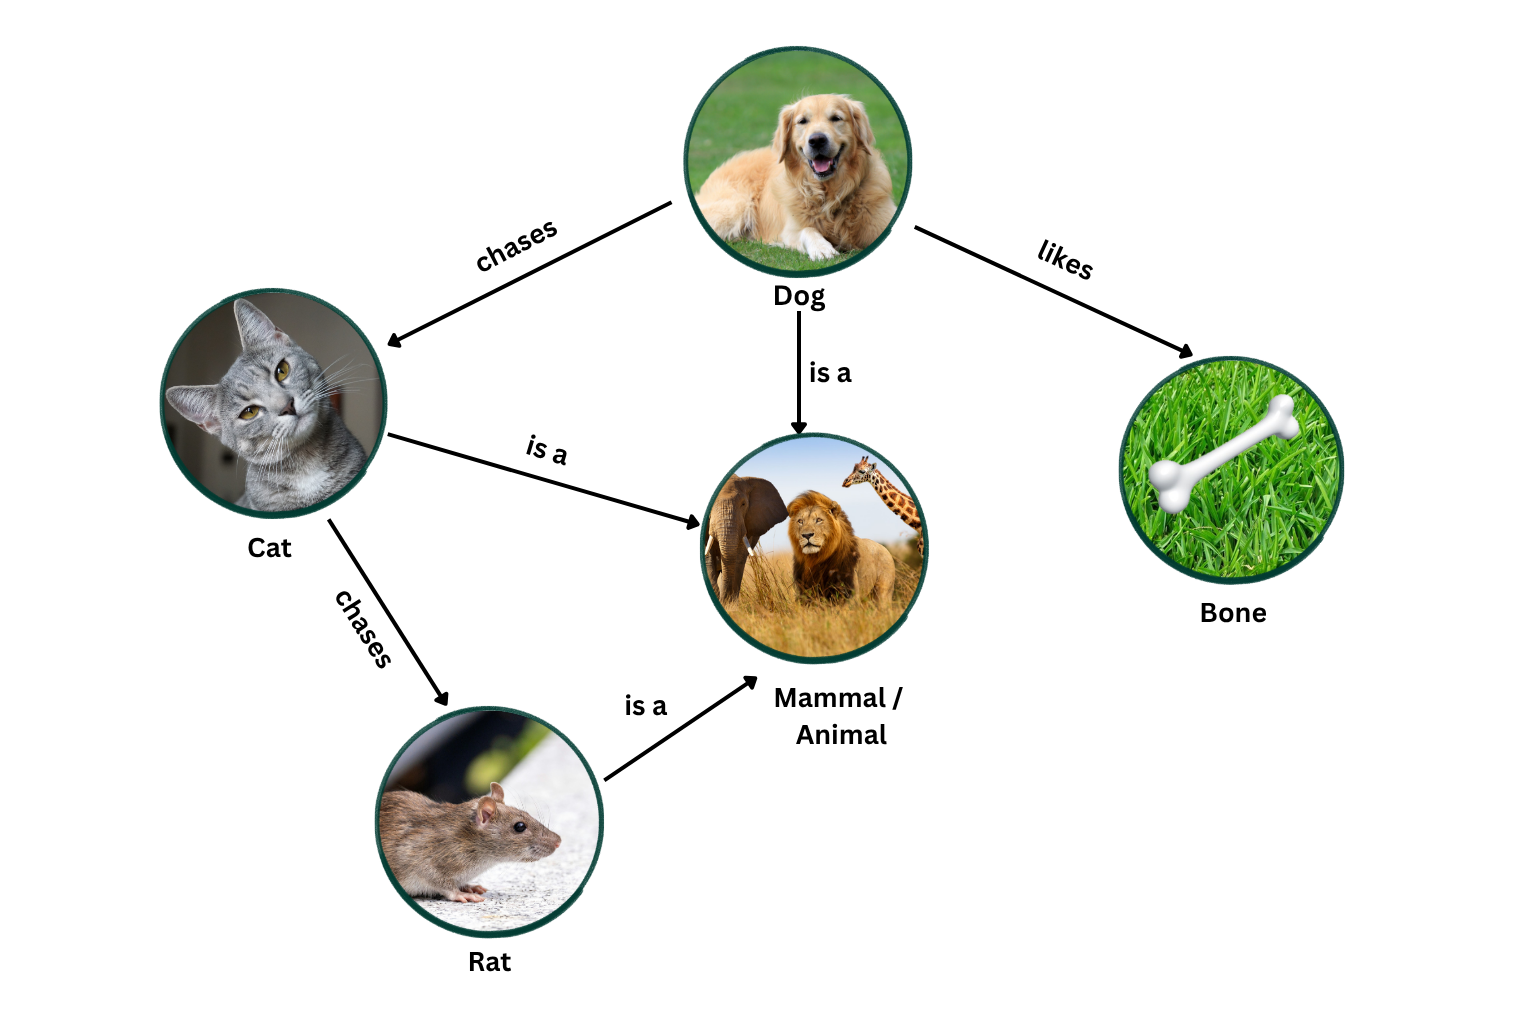
\includegraphics[width=\textwidth]{inc/figures/kg.png}
    \caption{Knowledge Graph Example}
    \label{fig:kgexample}
\end{figure}
For example, Figure~\ref{fig:kgexample} shows a small knowledge graph in
which entities such as a dog, cat, rat, and bone are represented as nodes,
while labelled edges represent relations between them, such as
\textit{chases}, \textit{likes}, and \textit{is a}. The example is deliberately
domain-independent and is intended only to illustrate the basic node--edge
representation of a knowledge graph. In this thesis, the same principle is
applied to clinical guideline concepts, with entities such as drugs,
conditions, guidelines, and clinical targets represented as typed nodes.
The complete clinical schema used in this work is defined later in
Section~\ref{sec:schema}.


\subsection{Graph Data Models}
\label{sec:bg-kg-models}

The internal model chosen for a knowledge graph determines how facts and their
attributes are stored and queried. ~\cite{hogan2021} describe
several models, of which two are relevant to this work: the directed
edge-labelled graph, of which the Resource Description Framework (RDF) is the
best-known instance, and the property graph.

In a directed edge-labelled graph, every fact is a triple that links a subject
node to an object node through a labelled edge, written here as
subject--predicate--object. Any additional detail about an entity, such as a
numerical value or a source reference, has to be expressed as further triples
attached to additional nodes, because an edge in this model carries only its
label~\cite{hogan2021}. RDF follows this model and adds conventions for naming
entities so that graphs published by different parties can be linked together.

A property graph relaxes this restriction. In addition to a type label, each
node and each edge may carry an arbitrary set of key-value
properties~\cite{hogan2021}. A fact such as a recommended dosage or the
guideline a statement came from can therefore be stored directly on the node
or edge it describes, rather than being broken out into separate triples.
~\cite{hartig2014} studies the correspondence between the two models and
shows how graphs can be translated between them, which confirms that the
choice is one of convenience and expressiveness rather than of what can in
principle be represented. The practical consequence is that attributes and
edge-level metadata are more compact to express in a property graph, a point
returned to when the schema of this work is defined in
Chapter~\ref{chap:construction}.

Table~\ref{tab:lpg-rdf} summarises the principal differences between the two
models across the dimensions most relevant to this work.

\begin{table}[htbp]
\centering
\small\setlength{\tabcolsep}{5pt}
\begin{tabular}{p{2.6cm} p{5.2cm} p{5.2cm}}
\hline
\textbf{Feature} & \textbf{Property graph} & \textbf{RDF} \\
\hline
Data structure
  & Typed nodes and edges, each carrying a set of key-value properties
  & Triples: subject -- predicate -- object \\[4pt]
Edge attributes
  & Stored directly on the edge as properties
  & Require intermediate nodes or reification triples \\[4pt]
Schema
  & Optional; the model can be extended at runtime
  & Ontology-driven; defined using RDFS or OWL \\[4pt]
Query language
  & Cypher (used in Neo4j and Memgraph)
  & SPARQL \\[4pt]
Interoperability
  & Local identifiers; suited to single-system deployments
  & Global URIs; supports linked open data across systems \\[4pt]
Primary strength
  & Graph traversal and analytics on highly connected data
  & Semantic reasoning and cross-system data integration \\
\hline
\end{tabular}
\caption{Comparison of property graph and RDF data models.}
\label{tab:lpg-rdf}
\end{table}

\subsection{Knowledge Graphs in the Biomedical Domain}
\label{sec:bg-kg-biomed}

In medicine, knowledge graphs are used to bring together information that is
otherwise scattered across terminologies, structured records, and the research
literature. A common starting point is a controlled vocabulary that assigns a
single identifier to each clinical concept. The Unified Medical Language System integrates many such biomedical
vocabularies into one resource, linking multiple names to a single concept and
providing tools for extracting concepts from text \cite{bodenreider2004}. Ontologies built on standard coding systems, such
as the drug ontology of ~\cite{hanna2013} based on RxNorm, serve a
similar role by providing stable identifiers that let independently produced
data be aligned.

Other work builds biomedical knowledge graphs from clinical text rather than
from vocabularies alone. ~\cite{li2020} construct a medical knowledge
graph from real-world clinical data and apply it to downstream tasks, while
~\cite{harnoune2021} use a BERT-based language model to extract
clinical entities and relations from biomedical documents for graph
construction. These systems generally draw on a single kind of source, most
often electronic health records or the biomedical literature. Knowledge graphs
built specifically from published clinical guidelines, and in particular from
several guidelines issued by different organisations so that their
recommendations can be compared, have received far less attention. That
setting is the focus of this thesis.

\section{Information Extraction}
\label{sec:bg-ie}

Building a knowledge graph from documents requires identifying the entities
mentioned in the text and the relations that hold between them. This section
describes the task and the main families of methods used to perform it.

\subsection{Named Entity Recognition and Relation Extraction}
\label{sec:bg-ie-ner}

The extraction task is usually divided into two parts. Named entity
recognition locates mentions of entities in text and classifies them into
types, such as a drug or a disease. Relation extraction then determines how
those entities are connected, for example that a drug is recommended for a
condition~\cite{nasar2021}. Together the two tasks turn unstructured text into
the typed nodes and edges that a knowledge graph is composed of. Both are
long-standing problems in natural language processing, and ~\cite{nasar2021} survey the range of methods that have been applied to
them.

\subsection{Rule-Based and Learning-Based Methods}
\label{sec:bg-ie-methods}

Approaches to information extraction fall broadly into rule-based and
learning-based methods. Rule-based extraction relies on hand-written patterns,
such as regular expressions or dictionaries of known terms, that match the way
information is stated in a particular kind of text.\cite{chiticariu2013} observe that rule-based information extraction dominates
the commercial world even though it is widely regarded as a dead end in
academic research, and note that practitioners value rule-based systems for
their interpretability. Rules are also a natural fit for text where the
relevant facts follow a predictable form, such as a numerical threshold or a
graded recommendation, because a small number of patterns can cover most of the
cases.
Learning-based extraction instead trains a model on annotated examples. Deep
learning models, in particular hybrid and joint models for named entity
recognition and relation extraction, now represent the state of the art
\cite{nasar2021}, and pre-trained language models fine-tuned for relation
extraction have outperformed earlier systems on clinical shared tasks
\cite{wei2020}. In the clinical domain, \cite{harnoune2021} use a BERT-based
model with a conditional random field layer to extract entities and relations
from clinical notes. Shared tasks such as the i2b2 and n2c2 challenges evaluated
systems for extracting concepts, assertions, medications, adverse drug events
and the relations between them from clinical narratives
\cite{uzuner2011,henry2020}. Learning-based methods depend on annotated
training data, which is scarce for many domains, and understanding the
decisions made inside deep architectures remains difficult \cite{nasar2021}.

\subsection{Hybrid Approaches}
\label{sec:bg-ie-hybrid}

Because the two families have complementary strengths, some systems combine
them.~\cite{chiticariu2013} argue for rule-based components
where precision and control matter, and hybrid designs that pair hand-written
rules with machine learning have been used in text-processing tasks to obtain
the reliability of rules together with the coverage of learned
models~\cite{villena2011}. Large language models have more recently been applied
to extraction as a further alternative, discussed in the next section. The
extraction stage of this work draws on a combination of rule-based and
learning-based methods, assigning each to the part of the task for which it is
better suited; the details are given in Chapter~\ref{chap:construction}.

\section{Grounding Language Model Output}
\label{sec:bg-grounding}

Large language models can produce fluent and plausible text, but they are
prone to generating statements that are not supported by any real source. This
section describes the problem and the techniques used to constrain model output
to reliable information.

\subsection{Hallucination in Language Models}
\label{sec:bg-grounding-hallucination}

The generation of unsupported or incorrect content by a language model is known
as hallucination. ~\cite{huang2025} distinguish two forms.
Factuality hallucination is when the output contradicts verifiable facts about
the world. Faithfulness hallucination is when the output departs from the input
or context the model was given, even where it is not wrong in a general sense.
They attribute this behaviour in part to the fact that the models are trained
to produce coherent and probable text, which does not by itself guarantee that
the text is factually correct. In a clinical setting this is a serious concern,
because a confidently worded but incorrect statement about a treatment or a
threshold could mislead a reader who is not in a position to check it.

\subsection{Retrieval-Augmented Generation}
\label{sec:bg-grounding-rag}

One established way to reduce hallucination is to ground generation in an
external source of knowledge rather than relying on what the model has stored
in its parameters. ~\cite{lewis2021} introduce retrieval-augmented
generation, which combines the parametric memory held in the model's weights
with a non-parametric memory in the form of an external document store. At
generation time the system retrieves relevant passages and conditions the
output on them, so that the generated text is tied to retrieved evidence. The
authors report that this grounding improves factual accuracy and provides a way
to trace an output back to the source it was drawn from. The same principle
underlies a range of later systems that constrain a language model to
information supplied at generation time rather than allowing it to draw freely
on its parameters.

\subsection{Schema-Constrained Generation}
\label{sec:bg-grounding-schema}

Providing a model with an explicit, structured input is a strong form of this
grounding. ~\cite{caufield2024} show that prompting a language
model with a defined schema constrains its output to the structure and content
requested, which is useful when the goal is to extract or generate information
that must conform to a fixed set of types. The question generation stage of
this work follows the same idea: rather than asking a language model to produce
clinical questions from its own knowledge, it supplies a single fact drawn from
the knowledge graph and constrains the model to that fact. Grounding of this
kind has been studied mainly for retrieval from text corpora; grounding
generation in a structured knowledge graph built from clinical guidelines, so
that every generated question is tied to a specific guideline statement, is
less commonly addressed. How this is done, and how the output is checked
against the supplied fact, is described in Chapter~\ref{chap:construction}.

\section{Automatic Question Generation}
\label{sec:bg-qg}

Generating questions automatically from a source of knowledge is an active
area of research in natural language processing, motivated by applications
in education, information retrieval, and dialogue systems. This section
reviews the main approaches and the educational framework used to describe
what different kinds of questions demand from a learner.

\subsection{Approaches to Question Generation}
\label{sec:bg-qg-approaches}

Early question generation systems used rule-based templates that transformed
a declarative statement into an interrogative form by pattern substitution.
These systems produce grammatical output reliably but are limited to the
question types for which templates have been written and lack the flexibility
to vary phrasing. Neural approaches have since been developed that learn to
generate questions directly from text or from structured knowledge sources.
~\cite{guo2024} survey the range of neural methods applied to
question generation, covering inputs including free text, knowledge bases, and
images. They report that knowledge-base question generation, where the input
is a set of structured facts rather than a passage of text, poses particular
challenges because the model must convert a formal relation triple into a
natural language question that accurately reflects both the entities and the
direction of the relationship.

Large language models have also been applied to knowledge-base question
generation, for example in few-shot settings where labeled data is scarce.
\cite{liang2023} propose KQG-CoT, which retrieves supportive logical forms
from an unlabeled pool and prompts an LLM to build a complex question as a
chain of sub-questions. A variant, KQG-CoT+, orders the demonstrations by
complexity and improves on the previous few-shot state of the art on
PathQuestions. \cite{guo2024} note in their survey that the central challenge
for LLM-based KBQG is designing prompts that steer the model toward the
intended question.

Question generation from clinical knowledge has received some specific
attention. ~\cite{nyameino2020} describe a system that
generates questions automatically from a clinical guideline, using the
guideline structure to drive the question type and content. The questions
produced cover individual recommendations taken from the guideline, rather
than comparing recommendations across several guidelines from different
organisations.

\subsection{Multiple-Choice Question Generation}
\label{sec:bg-qg-mcq}

Multiple-choice questions require, in addition to a correct answer, a set of
plausible but incorrect options, known as distractors, that a learner who does
not know the material might plausibly select. \cite{gao2019} address
distractor generation for reading comprehension questions, using a
hierarchical encoder-decoder with attention to generate longer, semantically
rich distractors from the article, the question, and the correct option. In a
clinical context, plausible distractors are typically other drugs or other
thresholds from the same domain, which makes a knowledge graph a natural
resource for distractor selection because it contains the set of all relevant
alternatives as named nodes.

\subsection{Educational Taxonomies and Difficulty}
\label{sec:bg-qg-bloom}

The cognitive demand of a question is typically described using a taxonomy of
learning objectives. ~\cite{anderson2001} revised the
original taxonomy proposed by Bloom to organise cognitive processes along six
levels: remember, understand, apply, analyse, evaluate, and create. The
revision shifted the original noun-based category names to verbs in order to
emphasise that these are active processes, and it moved the creation category
to the highest level to reflect that generating new constructs requires more
than evaluation alone. The lower levels, remember and understand, correspond
broadly to the ability to recall and interpret factual information, while
apply, analyse, and evaluate require the learner to use and reason with that
information in increasingly open-ended ways.

In question design, this hierarchy is used to classify the cognitive level a
question targets. A question that asks for the value of a specific diagnostic
threshold requires recall; a question that presents a clinical scenario and
asks which management option is appropriate requires application. Generating
questions at a range of levels produces a catalogue that tests different
depths of understanding rather than a single level of recall. This work
assigns a difficulty level to each generated question based on the relation
type that the question was built from, using the Bloom hierarchy as a guide,
as described in Chapter~\ref{chap:construction}.

Table~\ref{tab:bloom} shows the six cognitive levels of the revised taxonomy
together with the kind of question activity associated with each, based on
~\cite{anderson2001}.

\begin{table}[htbp]
\centering
\small\setlength{\tabcolsep}{5pt}
\begin{tabular}{p{0.5cm} p{2.2cm} p{7.8cm}}
\hline
& \textbf{Process} & \textbf{Associated question activity} \\
\hline
& Remember    & Recall or recognise a specific fact, term, or value \\[3pt]
& Understand  & Explain or restate a concept in one's own words \\[3pt]
& Apply       & Use a known fact or procedure to answer a new question or solve a case \\[3pt]
& Analyse     & Break a scenario into parts and identify how they relate \\[3pt]
& Evaluate    & Judge or justify a clinical decision against given criteria \\[3pt]
& Create      & Design, compose, or propose something novel from existing knowledge \\
\hline
\end{tabular}
\caption{Cognitive levels in the revised Bloom taxonomy.}
\label{tab:bloom}
\end{table}

\section{Clinical Practice Guidelines}
\label{sec:bg-guidelines}

Clinical practice guidelines are systematically developed statements that
summarise the available clinical evidence on a topic and translate it into
recommendations for practice \cite{nyameino2020}. Their purpose is to improve
the quality of care and reduce unjustified variation in practice
\cite{peleg2013}. Many guidelines grade the quality of the underlying evidence
and the strength of each recommendation, most commonly using the GRADE system
\cite{guyatt2011}. In the diabetes domain
the organisations whose guidelines are used in this work each produce such
statements independently, drawing on their own review processes and addressing
their respective healthcare systems and populations.

\subsection{Evidence Grading and Recommendation Structure}
\label{sec:bg-guidelines-grade}

Many guideline producers use a structured grading system to convey the
strength of the underlying evidence and the force of each recommendation.
One widely used framework is the Grading of Recommendations Assessment,
Development and Evaluation system, known as GRADE, which rates the quality of
evidence and grades recommendations as strong or weak according to the quality
of the evidence and the balance of desirable and undesirable consequences
\cite{guyatt2011}.
Under GRADE, evidence quality is rated from high to very low depending on study
design, consistency of findings, and precision, and recommendations are then
graded as strong or conditional based on both the quality of evidence and the
balance of benefits against harms. The GRADE system produces recommendations
that carry explicit markers of how much confidence a clinician should place in
them, which makes the recommendation label a meaningful structured field rather
than a narrative qualifier.

In practice, the issuing organisations whose guidelines this work uses do not
all follow exactly the same grading system. The ADA uses lettered grades
(A through E), NICE uses strength ratings tied to the quality of its evidence
review, and Diabetes Canada uses a graded classification from A to D.
Regardless of the specific notation, all four organisations distinguish
stronger from weaker recommendations in a structured way, and this structure
is part of what the ingestion stage of this work captures.

\subsection{Computer-Interpretable Guidelines}
\label{sec:bg-guidelines-cig}

Making guideline content available to computational systems requires moving
beyond the PDF and word-processed documents in which guidelines are typically
published. ~\cite{peleg2013} provides a methodological review of
computer-interpretable guidelines, a line of research that formalises clinical
guidelines as executable or queryable representations. The review covers
modelling languages and acquisition methodologies developed over roughly two
decades, and it identifies as a central challenge the gap between the natural
language in which clinical guidelines are written and the formal structures
that a computer can evaluate. The representations covered by Peleg range
from flow-chart-based models to logic-based formalisms, and the work reports
that translating a narrative guideline into any of these forms remains
time-consuming and requires significant expert input.

Approaches that use artificial intelligence to assist or automate this
translation have attracted increasing interest. Large language models can
extract structured information from text with little or no task-specific
training data \cite{xu2024, caufield2024}, which suggests they could also help
turn narrative guidelines into structured form. This thesis takes a related
but distinct approach: rather than formalising a guideline into a decision
model, it extracts the entities and relations that a guideline states into a
property graph, so that the content of several guidelines can be queried and
compared in a common structure. The difference is in purpose:
computer-interpretable guidelines aim at decision support and care pathway
execution, while the knowledge graph constructed in this work aims at
information integration and study question generation across multiple
guideline sources. Question generation in this setting has so far mainly
supported guideline development: \cite{sousa-pinto2024} prompted LLMs to
propose guideline questions and found that some were not previously raised by
the guideline panel.

\section{Related Work}
\label{sec:bg-related}

This section discusses the work most closely related to this thesis and sets
out how the present work differs from it. The preceding sections have
reviewed individual technical components in isolation; here the focus is on
systems that combine several of those components toward a goal comparable to
the one pursued here.

\paragraph{Knowledge Graph Construction from Clinical Text}
\label{sec:bg-related-kg}

Several systems construct biomedical knowledge graphs from clinical text
using extraction pipelines that combine named entity recognition with relation
extraction.~\cite{li2020} build a medical knowledge graph from
real-world clinical data records, and ~\cite{harnoune2021}
extract clinical knowledge from biomedical documents using a BERT-based model.
Both systems work on a single document collection of one type, either
electronic health records or biomedical literature, and neither addresses the
problem of combining content from multiple separately produced guidelines that
each use different structural conventions and different units of measurement.
The present work is distinguished by its explicit treatment of structural
heterogeneity across sources and its normalisation of measurement units so
that numerical thresholds from different guidelines can be directly compared.
\paragraph{Question Generation from Clinical Knowledge}
\label{sec:bg-related-qg}

Question generation from structured knowledge has developed as a distinct
research direction as knowledge graphs have grown richer and more queryable.
~\cite{bi2020} generate questions from knowledge bases using
explicit type constraints and grammar guidance, showing that the structural
properties of a knowledge source can be used to control the factual content
and form of generated questions. ~\cite{guo2024} survey neural question generation across knowledge bases, text, and images,
organize the literature into structured, unstructured, and hybrid NQG, and
note that knowledge-base question generation benefits from models that
preserve graph structure and mark the roles of heads, relations, and tails
rather than treating a subgraph as a flat sequence of triples. Prompting a language model with structured input rather than asking it to
generate freely is a common design in knowledge-base question generation
\cite{liang2023}, and constraining output to supplied content is also used to
reduce unsupported statements \cite{huang2025}.

In the clinical domain specifically, ~\cite{nyameino2020}
describe a system that generates questions automatically from a single
clinical guideline for use in a gamified training setting. Their work is the
closest antecedent to the question generation component of this thesis and
establishes that guideline content can be turned into assessment questions
automatically.

This thesis extends that line of work in two ways. First, the input is a
knowledge graph built from four guidelines rather than a single source
document, which makes cross-guideline questions possible. Second, each
question is grounded to a specific graph edge selected before the language
model is called, and every generated question is validated against that
anchor. Questions derived from \textsc{equivalent\_to} edges, which connect
nodes from different organisations that assert the same numerical threshold,
require knowledge of how two guidelines compare and are not possible from a
single-guideline source.

\paragraph{AI-Assisted Guideline Processing}
\label{sec:bg-related-ai-guidelines}

\cite{sousa-pinto2024} examine how large language models can support the
development of guideline questions, using the ARIA 2024 guidelines as a single
case study, and \cite{peleg2013} reviews the broader effort to produce
computer-interpretable representations of individual guidelines for use in
decision support. Neither addresses the representation of several guidelines
together. The goal of this thesis is different: it is not to execute guidelines
as decision logic but to represent the content of several guidelines in a
common structure that can answer questions about how those guidelines agree,
differ, and complement one another.


\chapter{Knowledge-Graph-based Question Generation Pipeline}
\label{chap:construction}

This chapter presents a framework for turning a set of clinical guideline documents into a queryable Knowledge Graph, and for using that graph as a controlled source for generating questions. The four-stage architecture is not specific to diabetes, although the schema, extraction rules, canonical entities, and normalisation procedures used in this thesis are configured for the diabetes guideline corpus.

The chapter follows the same order the pipeline runs in. Section~\ref{sec:corpus} describes the corpus: which documents are used and why. Section~\ref{sec:ingestion} presents the document structuring stage, in which each document is parsed into typed 
element records with page-level provenance. Section~\ref{sec:schema} 
defines the graph model — the node types, relation types, and 
formal properties of the graph. Section~\ref{sec:extraction} 
describes the dual-layer approach to identifying entities and 
relations in the preprocessed records. Section~\ref{sec:normalisation} 
explains how extracted records are deduplicated, unit-normalised, 
and integrated into a single graph. Section~\ref{sec:questions} 
describes how the finished graph is used as a controlled source 
for question generation.

\section{Overview and Objectives}
\label{sec:overview}

The goal of this work is to build a Knowledge Graph that combines several diabetes guidelines into one structured, queryable representation, and to use that graph to generate questions automatically. Eight documents from four organisations are used, covering diagnosis, screening, glycaemic targets, pharmacological management, and monitoring across both Type~1 and Type~2 diabetes. The pipeline is organised into four stages: ingestion, extraction, normalisation, and question generation. This four-stage architecture is not inherently specific to diabetes, but its implementation in this thesis is configured for the diabetes guideline corpus. This includes publisher-specific document-structuring rules, the Knowledge Graph schema, clinical extraction patterns and canonical entities, unit-normalisation procedures, and the relation-to-question mappings. Applying the same architecture to another clinical domain would therefore require adapting these domain- and corpus-specific components. Diabetes guidelines are used as the test domain mainly because they are structurally messy in different ways depending on the publisher, which meant the pipeline had to be tested against a real spread of formats, not one clean case.

This objective breaks down into three concrete reasons for building the graph in the first place.

\paragraph{Cross-guideline comparison}
Once each guideline's content is represented as typed nodes and edges, queries can compare positions across organisations, for example by identifying guidelines that specify the same normalised glycaemic target or recommend the same drug as first-line therapy. Numerical targets are kept organisation-specific and are compared only after unit normalisation, as described in Section~\ref{sec:unit-normalisation}. The resulting cross-guideline comparisons for the diabetes corpus are reported in Chapter~\ref{chap:evaluation}.

\paragraph{Structured accessibility of clinical knowledge }
Guidelines are written for clinicians to read, not for software to parse \cite{peleg2013}. Everything is embedded in prose, numbered lists, and tables, none of which is machine-readable on its own; Section~\ref{sec:bg-ie} discusses this in more depth. Converting that content into a property graph is what makes it possible to query and visualise it, not just search it as text \cite{li2020,harnoune2021}.

\paragraph{Question generation for clinical education }
Once the guideline content sits in a graph, question generation can work directly off graph edges, without needing unstructured passages \cite{guo2024,bi2020}. Selected clinical and cross-guideline edges represent statements extracted from or derived from the source guidelines and can be used as anchors for questions at several difficulty levels, which is useful for building learning or assessment material. The question types used here are defined in Chapter~\ref{chap:background}.

\subsection*{Challenges}

The construction of a multi-guideline knowledge graph introduces five challenges that do not arise in a single-source setting.

Challenge~1 is structural heterogeneity. Because the guidelines come
from distinct publication workflows, there is no uniform document
structure. While some publishers provide clean Unicode text, others
introduce extraction artefacts such as missing whitespace. A fixed
document-structuring procedure therefore cannot be applied unchanged
across the entire corpus. The framework must accommodate
publisher-specific structural differences while producing the same
typed intermediate representation for downstream processing. The
specific repair procedures required for the diabetes corpus are
described in Chapter~\ref{chap:evaluation}.

Challenge~2 is terminological variation. The same clinical idea may be worded differently across organisations. For example "type~2 diabetes" versus "non-insulin-dependent diabetes mellitus" for the same condition. If these forms are kept
as separate identities, relations that should meet at one node are
split across several nodes. The graph therefore needs a canonical form
for such variants before cross-guideline queries are meaningful.

Challenge~3 is unit inconsistency. The guidelines do not consistently use the same measurement units.  A numerical comparison is useless if
the values are not first put on the same scale. A fasting plasma glucose
threshold may be written as 126~mg/dL in one representation and
7.0~mmol/L in another. The numbers look different even though conversion
places them at the same threshold. Cross-guideline comparison therefore
requires unit normalisation before numerical targets are compared.

Challenge~4 is controlling information the language model
introduces beyond what the input actually states. Clinical guideline
text is safety-sensitive: an invented drug indication or a fabricated
contraindication would misrepresent an actual clinical guideline, which
is a more serious failure mode than in general-purpose text generation
\cite{huang2025}. The risk is not limited to entity extraction. In
question generation, a graph anchor may specify an HbA1c threshold without specifying a patient age. A generated vignette that introduces a numerical age has therefore added information not contained in the anchor.
This risk is why the extraction and question-generation stages
(Sections~\ref{sec:extraction} and~\ref{sec:questions}) are built the
way they are: the language model is instructed to classify or rephrase
information already present in the structured input rather than
introduce additional clinical facts, and its output is checked against
that input wherever possible. 

Challenge~5 is entity scoping. Some concepts should be shared across the
whole graph, while others must retain the organisation that stated them.
A Drug such as metformin can be represented by one global node even when
several guidelines mention it. A numerical target is different. If ADA
and IDF both state an FPG threshold of 7.0~mmol/L, the two target nodes
remain separate because they represent independent guideline statements.
Their agreement is represented by an \textsc{equivalent\_to} edge rather
than by merging the nodes. This distinction is fixed by the schema and
carried through deduplication and normalisation.

\subsection*{Contributions}

The pipeline consists of four main technical components.

The first is separating entity types into two extraction layers before any extraction runs. This differs from the hybrid approaches of running rules first and letting a language model fill the gaps (or the reverse). Both of those patterns let the two methods work on the same categories, which makes it hard to tell afterwards which method produced which result, or to attribute errors. Here, each entity type is assigned up front to either the rule-based layer, if it has a consistent lexical or typographic pattern, or the language-model layer, if picking it out requires understanding context. Extraction-derived records retain method metadata where applicable, allowing the contribution of each extraction route to be inspected separately.

The second is constraining the language model's extraction output to a fixed schema. The model is given the allowed node and edge types as a prompt-level constraint and is only supposed to classify what is already in the passage, not add to it. This matters more here than in a general information-extraction task, because a model that invents a category or a drug indication produces a graph that looks fine and is wrong in a way a reviewer might not catch.

The third is anchoring every generated question to a specific graph edge
before the language model is called. Source relations retain organisation
and page provenance where available, while derived relations retain their
source context through the graph elements from which they are constructed.
When an eligible edge is selected as a question target, the available
provenance is retained with the anchor. The model is provided with the
anchor as its factual input and is instructed not to introduce information
beyond it. The graph decides what is asked; the model decides how it is
phrased.

The fourth is creating cross-guideline equivalence edges after unit normalisation. This works better than trying to extract them from the text directly, since no single guideline document ever states that its own target is equivalent to another organisation's target. For plasma-glucose targets, values expressed in different source units are normalised to mmol/L. Two \textsc{GlycaemicTarget} nodes from different guidelines that share the same metric, operator, and rounded normalised value are then linked with an equivalence edge. This relation only exists because the graph combines multiple guidelines; it could not come out of any single-guideline pipeline.

\begin{figure}[!ht]
    \centering
    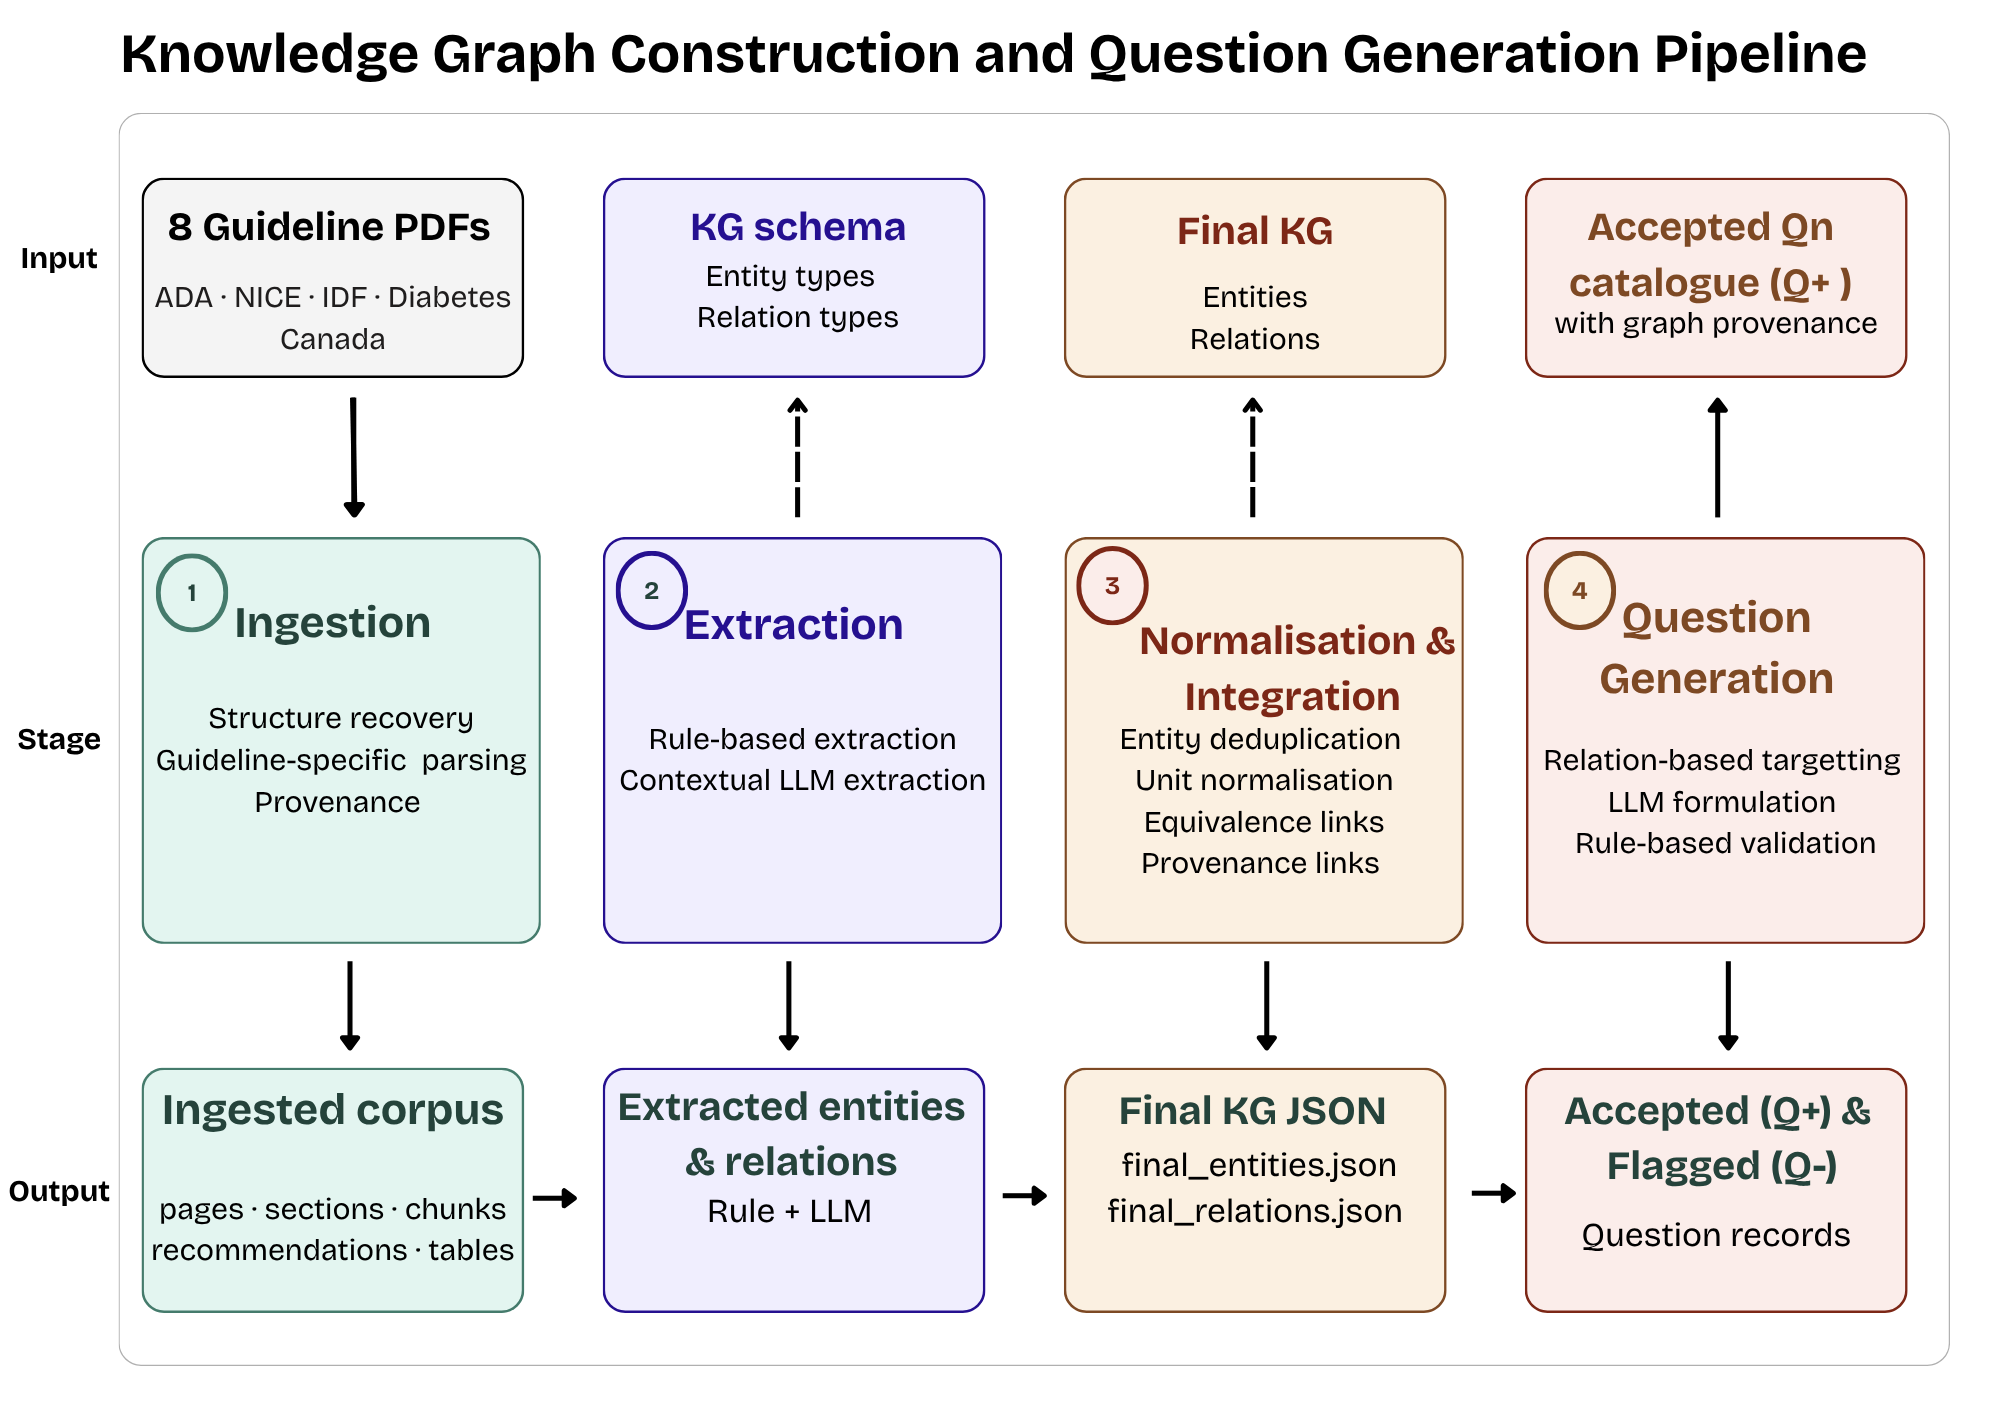
\includegraphics[width=\textwidth]{inc/figures/pipeline.png}
    \caption{Four-stage knowledge graph construction pipeline.}
    \label{fig:pipeline}
\end{figure}

Figure~\ref{fig:pipeline} shows the pipeline end to end. Guideline documents go into ingestion, which produces a structured representation of each document's content. Extraction reads that representation and produces two sets of typed entity and relation records, one from the rule-based layer and one from the language-model layer. Normalisation merges those two sets into one graph. Records referring to the same real-world entity are deduplicated into a single node, and numeric thresholds are converted to a common unit so equivalence edges can be detected. Question generation then walks the finished graph, selects eligible edges as anchors, and produces a validated set of clinical questions retaining the provenance available on their source graph relations

\section{Corpus Design}
\label{sec:corpus}

Building a Knowledge Graph that supports cross-guideline comparison requires a corpus that covers one clinical topic but varies in how that topic is presented. Using documents from a single organisation would produce a clean but narrow graph and defeat the purpose of cross-guideline comparison, so the corpus is selected against four criteria.

\paragraph{Geographic and systemic diversity}
Guidelines from different healthcare systems reflect different regulatory environments and patient populations. Using organisations from more than one country introduces variation in
guideline recommendations and healthcare-system context rather than only
the conventions of one national system.

\paragraph{Clinical coverage}
The selected guideline families need enough overlapping clinical content
for cross-guideline comparison to be possible. For this work, the common
coverage consists of diagnosis and classification, screening, glycaemic
targets, pharmacological management, and monitoring
\cite{ADA2026,NICE_T2_2026,IDF2025,CanadaDiabetes_Ch3}. A document covering
a narrower sub-topic can still be included where it contributes a
comparison point on one of these shared areas.

\paragraph{Format diversity}
Testing the pipeline against documents that all share one layout cannot show whether the pipeline generalises. The corpus requires documents that differ in how recommendations are laid out and in whether they use tables at all, so that ingestion and extraction face varied structure and not one convenient case.

\paragraph{Recommendation specificity}
Documents need to contain recommendations naming a specific drug, intervention, or measurement threshold, not high-level policy statements with nothing concrete to extract.

 The concrete outcome of applying these four criteria, i.e. which documents, how many pages, how many recommendations, is reported in Chapter~\ref{chap:evaluation}.

\subsection{Structural Heterogeneity as a Design Challenge}
\label{sec:heterogeneity}

Guideline documents from different organisations are not structurally uniform, and this shapes the design of every stage of the pipeline. Three dimensions of variation are particularly relevant to the pipeline.

\subsubsection{Recommendation format}

Some guidelines present recommendations as numbered, graded statements
that can be located by structural pattern. NICE's Type~2 diabetes
guideline uses this format throughout~\cite{NICE_T2_2026}:

\begin{quote}
\noindent
\textbf{1.13.1}\quad
\begin{minipage}[t]{0.82\linewidth}
For adults with type 2 diabetes and no relevant comorbidity, offer
modified-release metformin and an SGLT-2 inhibitor.
\hfill\textnormal{[2026]}
\end{minipage}
\end{quote}

The recommendation number, the imperative verb, and the update marker are
typographically consistent across the document and can be identified by
structural pattern matching. Metformin and SGLT-2 inhibitors are examples
of the \textsc{Drug} entities described in
Section~\ref{sec:node-types}.

The ADA Standards of Care also use numbered
recommendations, but place them within a multi-column layout alongside
commentary and cross-references~\cite{ADA2026}. For example:

\begin{quote}
\noindent
\textbf{9.21}\quad
\begin{minipage}[t]{0.82\linewidth}
In adults with type 2 diabetes without severe hyperglycemia or
hyperglycemic crisis, GLP-1-based therapy is preferred to insulin for
initial or add-on glucose-lowering therapy.
\hfill\textbf{A}
\end{minipage}
\end{quote}

Although both formats use numbered recommendations, their surrounding
document structure differs. The NICE recommendation can be located using
its consistent numbering and statement structure, whereas the ADA
recommendation must be identified within a three-column layout containing
additional commentary and cross-references. This difference affects how
the ingestion stage locates and extracts recommendation text.

\subsubsection{Tabular content}

Some guideline documents present diagnostic criteria in structured tables
rather than in numbered statements. This creates a different problem from
the numbering-versus-prose distinction above. The issue is not identifying
where a recommendation starts and ends, but reconstructing the row-and-column
structure before extraction can take place. The IDF and ADA documents present
some diagnostic criteria in this form. For example, ADA Table~2.1 includes
the following criteria~\cite{ADA2026}:

\begin{quote}
\textnormal{\textbf{Table 2.1: Criteria for the diagnosis of diabetes in
nonpregnant individuals}}\\[4pt]

FPG (fasting plasma glucose) $\geq 126$~mg/dL
($\geq 7.0$~mmol/L). Fasting is defined as no caloric intake for at least
8~h.\\[2pt]

\textit{OR}\\[2pt]

2-h PG (plasma glucose measured two hours into an OGTT, an oral glucose
tolerance test) $\geq 200$~mg/dL ($\geq 11.1$~mmol/L).
\end{quote}

When a naive text-stream extractor processes this page without spatial
reconstruction, the table structure collapses into a sequence of fragments
with no reliable row or cell boundaries. A simplified example of the
resulting text stream is shown below.

\begin{lstlisting}[
    language={},
    caption={Text-stream output from ADA Table 2.1 before spatial reconstruction.}
]
Table 2.1 Criteria for the diagnosis FPG 126 mg/dL 7.0 mmol/L
Fasting defined no caloric intake 8 h 2-h PG 200 mg/dL
11.1 mmol/L OGTT Random plasma glucose 200 mg/dL
\end{lstlisting}

Pattern matching for an expression such as
\texttt{FPG $\geq$ 126 mg/dL} fails on this output because the table
structure has collapsed and the comparison operators are not preserved in
the extracted text. The association between each metric and its corresponding
threshold can therefore no longer be recovered reliably from the text stream
alone. Spatial reconstruction of the row-and-column structure is required
before rule-based extraction of numerical thresholds from such pages.

The same extraction procedure cannot be assumed to apply to every guideline.
NICE NG17, for example, expresses comparable target information in prose
rather than in a table. Recommendation~1.6.6 states that adults with Type~1
diabetes should aim for an HbA1c level of 48~mmol/mol (6.5\%) or lower
\cite[recommendation 1.6.6]{NICE_T1_2022}. HbA1c (glycated haemoglobin) is
reported here in IFCC units (mmol/mol), which are discussed further below.
The ingestion pipeline therefore cannot assume that any single content
modality will be present across all guideline families.

\subsubsection{Measurement unit conventions}
Different organisations report the same class of measurement in different units. Plasma glucose values appear in mg/dL in the ADA document \cite{ADA2026} and in mmol/L in the NICE, IDF, and Diabetes Canada documents \cite{NICE_T2_2026,IDF2025,CanadaDiabetes_Ch3}. Glycated haemoglobin (HbA1c) appears as a percentage in some documents and in IFCC (International Federation of Clinical Chemistry) units (mmol/mol) in others; the standard method for relating the two scales is given by \cite{hoelzel2004}. Comparing numerical values across guidelines only works after unit normalisation, and only between values of the same kind. Cross-guideline comparison is restricted to targets that share the same
metric, operator, and normalised numerical value. The limitations of this
criterion are discussed in Chapter~\ref{chap:evaluation}.

These three dimensions of variation appear across all four guideline families in the corpus, and handling them without excluding a guideline family is a design requirement for the document-structuring and extraction stages described next.

Each of these three problems has been addressed individually in the
document-processing literature. PDF text extraction is a recognised difficulty
for scientific documents \cite{bast2017,ramakrishnan2012}, and tools such as
Docling combine layout analysis with table structure recognition
\cite{auer2024}. Table reconstruction has been studied for scientific articles
and document images \cite{zhong2020,schreiber2017}. Unit normalisation is
needed because clinical measurements are reported on different scales, for
example HbA1c in NGSP percent versus IFCC mmol/mol, which are related by a
linear regression \cite{hoelzel2004}. Here all three are handled within one
pipeline operating across four guideline families at once, without treating any
single family as the default case. The systems surveyed in
Section~\ref{sec:bg-related} address these problems individually, not in
combination.

\section{Structuring Guideline Documents for Extraction}
\label{sec:ingestion}

Clinical guideline documents are written for people, not software. Whatever format they arrive in, the actual clinical content is buried in a mix of typographic conventions, layout hierarchy, prose, numbered lists, and embedded tables, and none of that carries explicit markup a program can rely on. This is not really a PDF problem specifically. Human-oriented documents do not necessarily expose the semantic and structural information required by the downstream pipeline in a machine-readable form. Structuring the documents has three requirements. Each piece of content
needs a type, its position in the document structure needs to be retained,
and anything extracted from it later must remain traceable to the source.
The content model below represents these requirements explicitly.

\subsection{The Document Content Model}
\label{sec:content-model}

Ingestion works against a fixed content model. A guideline document $d \in \mathcal{D}$ is treated as an ordered sequence of content elements $e_1, e_2, \ldots, e_n$, and each element is a triple $e_i = (\tau_i,\ \text{text}_i,\ \pi_i)$, where $\text{text}_i$ is the extracted text, $\pi_i$ is a provenance record (defined below), and $\tau_i$ is drawn from a content-type set $\mathcal{T}_C$. $\mathcal{T}_C$ enumerates the structural units a document domain 
distinguishes, and in general it needs to separate free-form narrative 
content from any self-contained, explicitly delimited unit the document 
type uses. The distinction is structural, not semantic. A delimited unit has 
identifiable boundaries and usually a label the document itself 
supplies, so it can be located reliably and its identifier kept for 
provenance. Narrative text has neither. What $\mathcal{T}_C$ actually contains is a domain-specific configuration, not a fixed part of the model. For this corpus,
$$\mathcal{T}_C = \{\textsc{Prose},\ \textsc{Recommendation},\ \textsc{Table},\ \textsc{Section}\}$$
Chapter~\ref{chap:evaluation} describes how these four types were derived from the four diabetes guideline documents and gives the extraction rule used for each; a different document domain would likely need a different $\mathcal{T}_C$.

Each element's provenance has two levels. At the element level:
$$\pi_i^{\text{elem}} = (id_i,\ \text{sec\_id}_i,\ \text{sec\_title}_i,\ p_i^{\text{start}},\ p_i^{\text{end}})$$
$id_i$ is a unique element ID so anything extracted later can be traced back to it; $\text{sec\_id}_i$ groups elements by section for entity typing; $\text{sec\_title}_i$ is the actual heading text, which extraction uses to infer relation type; and $p_i^{\text{start}}, p_i^{\text{end}}$ are start and end page numbers, kept because any extracted claim needs to be checkable against the source page it came from. Elements of a self-contained, explicitly delimited type may carry an additional label field where the document itself provides one (e.g. a recommendation number), absent for other types. At the document level, a shared record resolves from $id_i$:
$$\pi_i^{\text{doc}} = (d_{\text{id}},\ \text{org},\ \text{geo},\ \text{source\_file})$$
covering the document ID, issuing organisation, healthcare system, and source filename.

Ingestion itself is a function $\varphi: \mathcal{D} \rightarrow 2^{\mathcal{E}}$, and it has to satisfy three things regardless of domain. \textit{Totality}: it produces output for every document, no document is allowed to come out empty just because, say, it lacks one particular content type. \textit{Type coverage}: across the whole corpus, every content type in $\mathcal{T}_C$ actually shows up at least once, so the ingestion logic cannot quietly collapse into handling only one modality. \textit{Provenance completeness}: every element that comes out has a fully populated $\pi_i$, so it can be traced back to a source location. Chapter~\ref{chap:evaluation} shows a concrete element produced by $\varphi$ for this corpus and how these three properties were verified against it.

\subsection{Structural Challenges in Ingestion}
\label{sec:ingestion-challenges}

PDF extraction is known to introduce artefacts like broken ligatures, lost word boundaries, and collapsed table columns \cite{bast2017,auer2024}. These are implementation-level engineering problems rather than conceptual ones, but the general requirement they impose on ingestion belongs here: the ingestion stage must detect and repair publisher-specific encoding artefacts before passing text downstream, since a corrupted token boundary breaks any pattern match or rule that assumes intact words. Two such challenges showed up often enough in this corpus to need dedicated handling; Chapter~\ref{chap:evaluation} gives the concrete encoding artefact encountered and the publisher-specific repair it required.

The first is extraction fidelity, i.e. documents from different publishers coming out of extraction looking very different internally, in ways that were not spread evenly across the corpus but tied to specific publishers' pipelines. A fix for this kind of artefact has to be written per publisher; one generic normalisation pass does not generalise across document families.

The second challenge is knowing where a recommendation actually ends. Even where the text extracts cleanly, grading scales, evidence summaries, and qualifying clauses sit typographically right next to the recommendation itself, and the boundary between "this is the recommendation" and "this is commentary about it" is not consistent across document families. No single rule covered all four families, so this was configured separately for each.

The complete set of typed, provenance-annotated elements from $\varphi$ is the only input the extraction stage (Section~\ref{sec:extraction}) receives --- no raw document text passes through beyond this point.

\section{Knowledge Graph Schema}
\label{sec:schema}

What the schema allows as a node or an edge determines what the graph can eventually be queried for. This section works through that schema in order: the formal graph model, then the node types, then the relation types, and finally why these particular types were chosen over the alternatives that were considered and dropped.

\subsection{Knowledge Graph Model}
\label{sec:graph-model}

The model used here is the labelled property graph, where nodes and edges are typed and can carry key-value properties \cite{hogan2021,hartig2014}. Formally, the graph is
\begin{equation}
G = (V,\ E,\ \mathcal{T}_V,\ \mathcal{T}_E,\ \phi,\ \psi,\ \lambda)
\label{eq:kg}
\end{equation}
where $\mathcal{T}_V$ is the node type set (Section~\ref{sec:node-types}) and $\mathcal{T}_E$ is the relation type set (Section~\ref{sec:relation-types}), defined before the rest of the tuple since both are used in what follows. $V$ is the set of nodes, and $E \subseteq V \times \mathcal{T}_E \times V$ is the set of directed typed edges, each edge $e = (v_i, r, v_j)$ connecting a source node to a destination node via a relation type $r \in \mathcal{T}_E$. $\phi: V \rightarrow \mathcal{T}_V$ assigns every node exactly one type, and $\psi: E \rightarrow \mathcal{T}_E$ assigns every edge exactly one relation type. $\lambda: V \cup E \rightarrow 2^{\mathcal{P}}$ maps nodes and edges to key-value properties; this is where clinical attributes and provenance metadata are stored.

Two things about the underlying requirements pushed this toward a property graph over RDF. In general, different entity types need different attribute sets: in this corpus, for example, a \textsc{GlycaemicTarget} node needs a metric name, an operator, a value, and a unit, while a \textsc{Drug} node needs none of those. A property graph handles this directly through $\lambda$. RDF would need a separate triple per attribute, splitting one clinical fact across several statements \cite{barrasa2023}. Provenance was the second factor. Clinical relationships need to remain
traceable to their source context, so provenance must be representable on
edges as well as on nodes. Property graphs support edge properties directly. RDF needs named-graph reification or the singleton property pattern to attach metadata to a statement, which adds structural overhead without a corresponding benefit for this use case.

The corpus $\mathcal{D} = \{d_1, d_2, \ldots, d_n\}$ is the only factual source for $G$. Building $G$ means applying the extraction function $\xi$ (Section~\ref{sec:extraction}) to the output of $\varphi$, then applying the normalisation function $\eta$ (Section~\ref{sec:normalisation}) to merge the result into a deduplicated instance of $G$.

\subsection{Node Types and Their Roles}
\label{sec:node-types}

The node type set is:
\begin{align*}
\mathcal{T}_V = \{\textsc{Organisation},\ \textsc{Guideline},\ 
\textsc{Condition},\ \textsc{Drug},\ \textsc{ClinicalCondition},\ \\
\textsc{Intervention},\ \textsc{Population},\ \textsc{GlycaemicTarget},\
\textsc{Recommendation},\ \\ \textsc{MonitoringProtocol},\ 
\textsc{Table},\ \textsc{Test},\ \\ \textsc{TreatmentRecommendation}\}
\end{align*}

These thirteen types came from inspecting the four guideline families in the corpus \cite{ADA2026,NICE_T2_2026,IDF2025,CanadaDiabetes_Ch3}, not from an existing medical ontology, and no claim is made that the same thirteen types would work in another clinical domain. An initial list was drawn from the recurring subjects of the recommendation statements, then went through two rounds of manual review. Types that could not be reliably populated from the corpus were dropped, and types that were quietly conflating two different subjects were split apart. The thirteen types split across three categories: global types,
organisation-scoped types, and structural types that sit outside both
scoping levels.

\subsubsection{Global node types}
A drug is the same drug no matter which guideline mentions it, and a clinical condition is the same condition no matter which body defines it. These concepts are represented as global nodes, independent of any one guideline, and that independence is what makes cross-guideline comparison possible in the first place. A single global \textsc{Drug} node can participate in \textsc{first\_line\_for} relations originating from several guidelines, allowing recommendations about the same drug to be compared directly. The global types are \textsc{Drug}, \textsc{Condition}, \textsc{ClinicalCondition}, \textsc{Intervention}, and \textsc{Test}.

\subsubsection{Organisation-scoped node types}
A glycaemic target value stated in one guideline is not automatically the same statement as a numerically similar value in another. Each is issued by a specific organisation, for a specific patient population, and merging the two on numerical similarity alone would erase that distinction. Organisation-scoped nodes keep each guideline's own position separate by carrying the issuing body as a required property. The organisation-scoped types are
\textsc{GlycaemicTarget}, \textsc{Recommendation},
\textsc{TreatmentRecommendation}, \textsc{MonitoringProtocol},
and \textsc{Table}.

\subsubsection{Structural node types}
Three types are structural, not clinical. \textsc{Organisation} nodes represent the guideline-issuing bodies and sit at the root of the provenance hierarchy. \textsc{Guideline} nodes represent individual published documents and connect to their issuing organisation by a \textsc{publishes} edge. Where a direct structural relation exists, such as \textsc{has\_recommendation} or \textsc{contains\_table}, the extracted node is linked directly to its source guideline; other organisation-scoped nodes retain guideline-level provenance through organisation and source metadata rather than a direct edge. \textsc{Population} nodes represent patient subgroups, letting the graph
distinguish a recommendation for all adults with Type~2 diabetes from
one aimed at a more narrowly defined subgroup. The corpus contains many
such subgroups stated at different levels of specificity, for example
distinctions by age, by pregnancy status, or by a named comorbidity.
Population is treated as structural, not global, because these
subgroup descriptions are worded differently across organisations and
in some cases across recommendations from the same organisation; in
the corpus, a subgroup only carries meaning in relation to the specific
recommendation and guideline that names it.
A small example shows why Population is kept structural. The
population descriptions are extracted contextually rather than by
fixed pattern. ADA recommendations reference an older-adult subgroup using several
different phrasings across different recommendations, including
"older adults with type~2 diabetes," "older adults," and
"individuals aged~70~years and older." These are not treated as one
canonical Population node the way \textsc{Drug} mentions of metformin
are, because merging them would erase which specific recommendation
each phrasing came from, and because the boundary of "older" is not
stated consistently even within a single guideline.


\subsection{Relation Types and Their Semantics}
\label{sec:relation-types}

The relation type set is:
\begin{align*}
\mathcal{T}_E = \{\ &\textsc{publishes},\ \textsc{has\_recommendation},\ \textsc{contains\_table},\ \\
&\textsc{first\_line\_for},\ \textsc{second\_line\_for},\ \textsc{recommended\_for},\ \\
&\textsc{contraindicated\_in},\ \textsc{manages},\ \textsc{used\_with},\ \\
&\textsc{associated\_with},\ \textsc{has\_target},\ \textsc{specifies\_target},\ \\
&\textsc{measured\_by},\ \textsc{requires\_monitoring},\ \textsc{has\_protocol},\ \\
&\textsc{describes\_protocol},\ \textsc{mentioned\_in},\ \textsc{equivalent\_to}\ \}
\end{align*}

These eighteen relation types are derived from recurring relationships
in the corpus together with the structural and provenance requirements
of the graph. Clinical relation types reflect relationships stated in
the guideline content, while structural and provenance relations encode
document organisation and traceability. The
\textsc{equivalent\_to} relation is different again: it is created
during normalisation rather than extracted from text.

Relation types are retained only where they represent a distinction
needed by the graph and could be populated reliably from the corpus. For
example, \textsc{first\_line\_for} and \textsc{second\_line\_for} remain
separate because merging them into \textsc{recommended\_for} would remove
the treatment-sequence distinction expressed in the source guidelines.

\subsubsection{Pharmacological relations}
These relations record treatment decisions. The guidelines give a drug's position in a treatment sequence, not just an association with a condition, so the schema needs to represent sequence. "First-line" and "second-line" refer to the order treatments are tried in, not to drug quality.

\textsc{first\_line\_for} and \textsc{second\_line\_for} are kept as separate types because the guidelines themselves use the terms "first-line" and "second-line" directly in the recommendation text \cite{NICE_T2_2026}. \textsc{recommended\_for} is a weaker type for cases where a guideline endorses a treatment without placing it in that hierarchy, which shows up often in guidelines whose tiered-care structure does not map cleanly onto first- or second-line. \textsc{contraindicated\_in} records that a drug should not be used in a given context; leaving it out would have meant the graph could only represent positive recommendations. \textsc{manages} links an intervention to a condition without naming a treatment-sequence position, which is common for non-pharmacological interventions such as lifestyle changes. \textsc{used\_with} records two agents named together in one recommendation. NICE recommendation 1.13.1 \cite{NICE_T2_2026} names modified-release metformin and an SGLT-2 inhibitor in a single statement, and representing that as two separate \textsc{first\_line\_for} edges would lose the fact that the source names them together. \textsc{associated\_with} is used for a weaker descriptive relation where
the source links a clinical concept to another concept without stating a
treatment recommendation, contraindication, or management relation.

Three relation types were considered here and dropped. \textsc{preferred\_over} would assert a direct comparative ranking between two drugs. In the four guidelines examined, preference between drugs was stated inconsistently and with population-specific qualifications attached, which made reliable extraction impractical; the same preference order can already be inferred by comparing the \textsc{first\_line\_for} and \textsc{second\_line\_for} edges on a shared condition node, so a dedicated relation was not needed. \textsc{dosage\_of} was dropped because dosage statements in the corpus are heavily conditioned on population, timing, renal function, age, and comorbidity, and a single binary edge cannot represent that. \textsc{causes}, for adverse effects, was dropped because adverse-effect statements are written in prose too variable to decompose reliably into clean drug-effect pairs.

\subsubsection{Monitoring and measurement relations}
A condition may be linked to a glycaemic threshold through
\textsc{has\_target}. This relation is created only when the surrounding
source context identifies the diabetes type unambiguously. If the context
does not distinguish Type~1 from Type~2 diabetes, the
\textsc{GlycaemicTarget} remains in the graph with its provenance but no
disease-specific \textsc{has\_target} relation is added. The target may
be linked to the relevant test through \textsc{measured\_by}, and a drug or condition may be linked to a monitoring protocol through
\textsc{requires\_monitoring}.

For example, when a passage explicitly identifies Type~1 diabetes and
states a numerical glycaemic target, the resulting target can be linked
to the global \textsc{Type 1 Diabetes} condition node. A numerical target
that does not establish whether the surrounding statement concerns
Type~1 or Type~2 diabetes is retained without such a condition-specific
edge. This avoids assigning a disease scope that is not supported by the
local source context.

\textsc{specifies\_target} links a \textsc{Recommendation} or \textsc{Table} node to the \textsc{GlycaemicTarget} it states explicitly. This edge is created only when the numerical target is extracted from an element with a known identity in the graph; targets extracted from general prose chunks, which have no such element to point back to, receive no \textsc{specifies\_target} edge. \textsc{has\_protocol} links a clinical concept to a
\textsc{MonitoringProtocol} associated with its monitoring requirements.
\textsc{describes\_protocol} links a source element, such as a
recommendation or table, to the \textsc{MonitoringProtocol} whose
procedural content it describes.

This chain exists because comparing thresholds across organisations is one of the central objectives of the graph, and that comparison needs a structured place to point to. \textsc{has\_target} points to a formally defined \textsc{GlycaemicTarget} node, which is what gets normalised and later carries an \textsc{equivalent\_to} edge. \textsc{requires\_monitoring} is kept separate from \textsc{has\_target} because a monitoring protocol is procedural, not numerical; it specifies what to check and how often, not a threshold value. \textsc{measured\_by} connects a  \textsc{GlycaemicTarget} to the diagnostic test used to assess it, and scopes the unit-normalisation problem: two targets for the same condition, measured by the same test but expressed in different units, become candidates for an \textsc{equivalent\_to} edge once normalised. A \textsc{frequency\_of} relation was considered but dropped, since monitoring-frequency statements in the corpus sit inside conditional clauses that would need a much richer event model to represent properly.

\subsubsection{Cross-guideline and provenance relations}
These relations give the graph its multi-guideline and provenance structure. They connect organisations, documents, extracted content, and cross-guideline comparison results.

\textsc{publishes}, \textsc{has\_recommendation}, and
\textsc{contains\_table} provide the main document-level provenance
links. An \textsc{Organisation} connects to its \textsc{Guideline}
nodes through \textsc{publishes}. A \textsc{Guideline} connects to its
\textsc{Recommendation} nodes through \\ \textsc{has\_recommendation} and
to its \textsc{Table} nodes through \textsc{contains\_table}. Together,
these relations preserve the connection between document content and
the organisation that issued the guideline.

\textsc{mentioned\_in} is a provenance relation linking a global entity to the guideline in which it occurs. These links are created during normalisation from the entity's recorded guideline mentions and are retained independently of any more specific clinical relations involving the same entity.

\textsc{equivalent\_to} is not extracted from text. It is created during
normalisation when two \textsc{GlycaemicTarget} nodes from different
guidelines share the same metric, operator, and normalised value after
unit conversion. It provides the mechanism used in this work to represent
cross-guideline agreement on a numerical threshold.

Two further types were considered and dropped from this group. \textsc{supersedes}, for one recommendation replacing an older one from the same organisation, would need a model of guideline update cycles over time, which is out of scope for a corpus frozen at a single point in time. \textsc{contradicts} was also considered, but disagreement between
organisations was not represented as an explicit relation in the source
documents. Differences can instead be identified by comparing
\textsc{first\_line\_for} or \textsc{has\_target} edges associated with
the same condition. Whether such a difference constitutes a clinical
contradiction is not determined by the graph.

\subsection{Schema Design Rationale}
\label{sec:schema-rationale}

The schema balances two requirements that pull in opposite directions.
It needs enough types to preserve distinctions that matter in the source
guidelines, but every additional type also has to be populated reliably.
For example, collapsing \textsc{first\_line\_for} and
\textsc{second\_line\_for} into \textsc{recommended\_for} would make
extraction simpler, but it would remove treatment order from the graph.
At the other extreme, a relation such as \textsc{dosage\_of} looks useful
in principle but would need more structure than a single edge can carry.
No systematic optimisation over alternative schema sizes is performed.
The retained types are those for which the distinction is useful to the
queries supported by the graph and for which the corpus provides enough
structure to populate the type consistently. The rejected relation types
and their individual reasons are discussed with the corresponding
relation groups above.

Figure~\ref{fig:schema} illustrates the node-scoping structure and representative relations in the Knowledge Graph. The node columns show representative node types from the global, structural, and organisation-scoped categories. The arrows show representative examples from the three relation groups: pharmacological, monitoring and measurement, and cross-guideline and provenance. The complete set of eighteen relation types is defined in $\mathcal{T}_E$ above.

\begin{figure}[!ht]
    \centering
    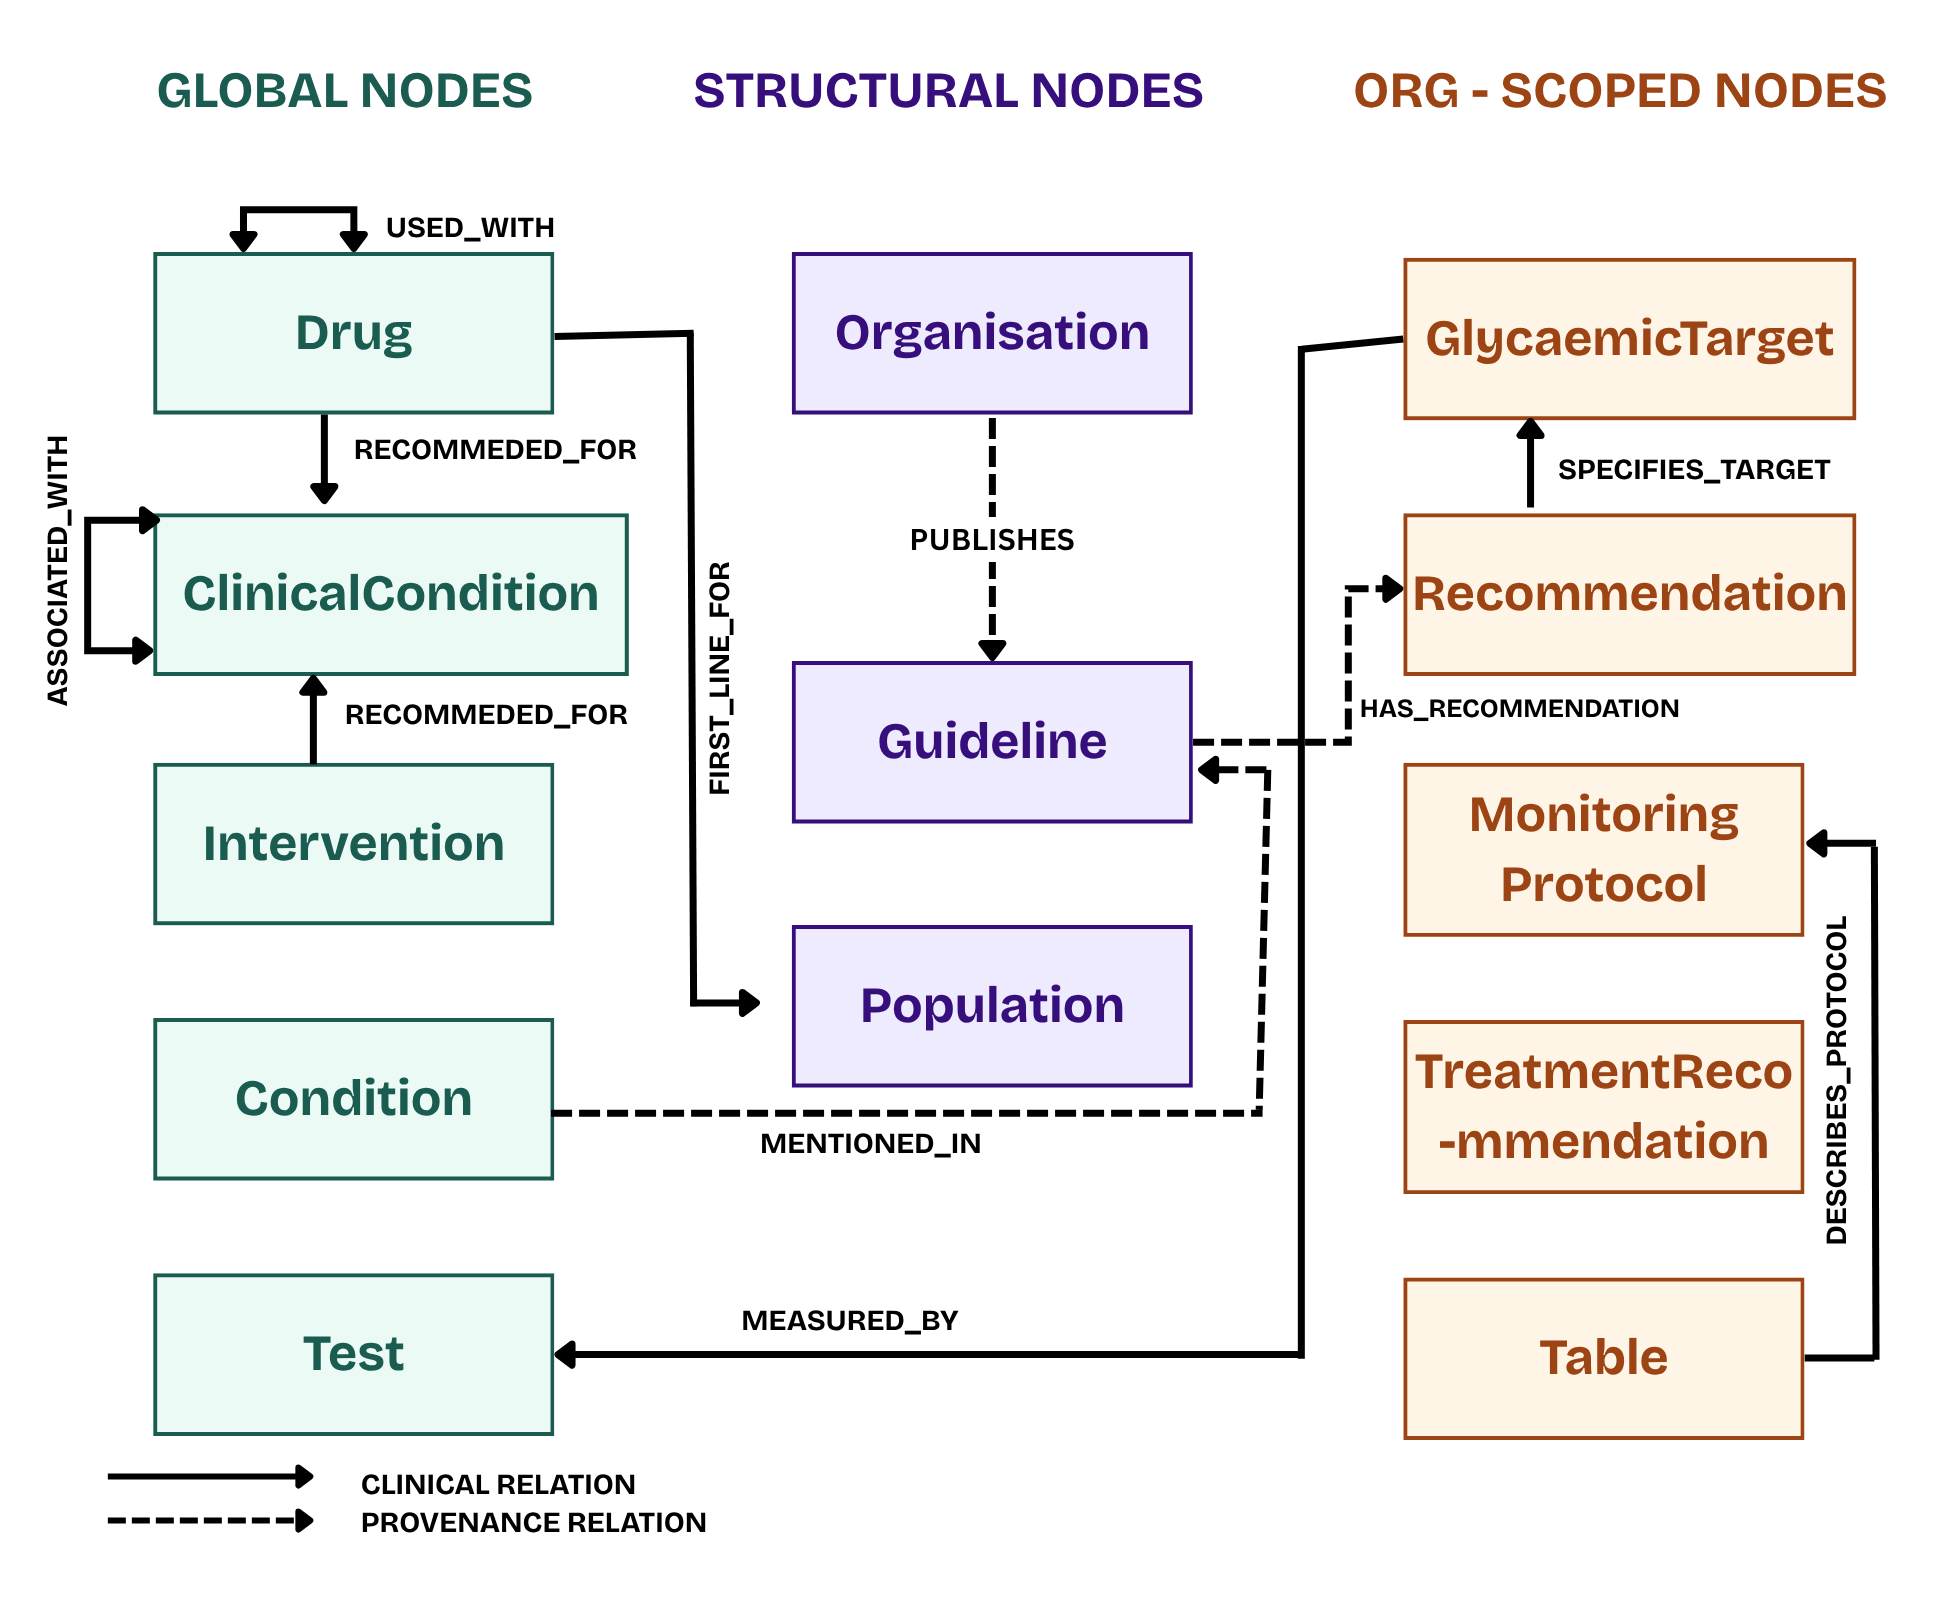
\includegraphics[width=\textwidth]{inc/figures/kg_schema.png}
    \caption{Knowledge Graph Schema}
    \label{fig:schema}
\end{figure}

Global nodes are what let edges cross between guidelines at all; leaving them out would mean each guideline produces its own isolated subgraph. Organisation-scoped nodes prevent the opposite problem. Leaving them out would merge every guideline's specific position into one shared node per concept, erasing the variation that cross-guideline comparison is meant to surface.

\section{Entity and Relation Extraction}
\label{sec:extraction}

The extraction stage reads the structured records produced by $\varphi$ and identifies the clinical entities and relations that become nodes and edges in the graph. This is where content elements from $\mathcal{T}_C$ turn into typed graph elements drawn from $\mathcal{T}_V$ and $\mathcal{T}_E$, and it is where the main architectural decisions sit. Three matter most. Which entity types go to which extraction layer, how the language model is constrained, and how identity is kept consistent across documents.

Two difficulties were particularly important in this corpus. The first is terminological precision. Clinical guidelines use controlled vocabulary where small differences in wording carry large differences in meaning; in the corpus documents, a drug described as "recommended" is not the same as one described as "preferred", which is not the same again as one "considered as an option". An extraction method that treats these as equivalent produces a graph that misstates how strongly a guideline actually recommends something. The second is cross-document consistency: the same concept can be worded differently across guidelines, for example "type~2 diabetes" in one and "non-insulin-dependent diabetes mellitus" in another, so extraction has to produce identifiers that match across documents, not only within one. Named entity recognition and relation extraction as techniques are background covered in Chapter~\ref{chap:background} \cite{nasar2021,zhao2024}; what this chapter contributes is not the techniques themselves but the specific architecture through which they are applied to a multi-guideline clinical corpus.

\subsection*{The Extraction Function}

Extraction is usually split into entity recognition and relation extraction as separate steps \cite{nasar2021}; here both are combined into one function:
\begin{equation}
\xi: 2^{\mathcal{E}} \rightarrow \mathcal{V} \times \mathcal{R}
\label{eq:extraction}
\end{equation}
where $2^{\mathcal{E}}$ is the power set of element records produced by $\varphi$, $\mathcal{V}$ is the set of typed entity records, and $\mathcal{R}$ is the set of typed relation records. An entity record $v \in \mathcal{V}$ is a tuple
$$v = (\text{id}_v,\ \tau_v,\ \text{name}_v,\ \pi_v,\ m_v)$$
where $\tau_v \in \mathcal{T}_V$ is the entity type, $\text{name}_v \in \mathbb{S}$ is the canonical surface form, $\pi_v$ is the provenance inherited from the source element, and $m_v \in \{\textsc{Rule}, \textsc{LLM}\, \emptyset\}$ records which layer produced it. A relation record $r \in \mathcal{R}$ is
$$r = (\text{id}_r,\ \text{src}_r,\ \psi_r,\ \text{dst}_r,\ \pi_r,\ m_r)$$
where $\psi_r \in \mathcal{T}_E$ is the relation type, $\text{src}_r$ and $\text{dst}_r$ are entity identifiers, $\pi_r$ is provenance, and $m_r$ is the method label. This method label is what makes each layer's contribution checkable on its own during normalisation and later evaluation, instead of only as a combined result.

\subsection{Rule-Based Extraction}
\label{sec:rule-extraction}

Rule-based extraction applies pattern matching and structural heuristics directly to the element records to pull out a specific, limited set of entity and relation types. Rather than trying to extract everything, the rule layer only targets types that have a reliable structural or lexical signal in the guideline text.

A type is assigned to the rule layer when its instances have a predictable
syntactic or structural form that is sufficiently consistent in the
document families where that type occurs. Types that do not meet this
condition are assigned to the contextual extraction layer.

\paragraph{GlycaemicTarget entities}
A numerical target has a local structure that can be decomposed directly.
For example,
\[
\text{FPG} \geq 7.0~\text{mmol/L}
\]
contains the metric \texttt{FPG}, the operator $\geq$, the value
\texttt{7.0}, and the unit \texttt{mmol/L}. These four fields are captured
separately by the rule layer: a regular expression matches the metric
name and unit as fixed anchors, with the operator and numeric value
extracted as separate groups in between. The gap between the metric
name and the operator is allowed to contain up to 40 or 60 characters
of intervening text, depending on the metric, so the same pattern still
matches when a guideline states the target inside a longer sentence
rather than as a short standalone expression. A second instance
illustrates this with a different metric and unit,
\[
\text{HbA1c} \geq 48~\text{mmol/mol},
\]
extracted by a separate but structurally identical pattern. The
surrounding sentence may vary, but the target itself retains the same
four-field structure in both cases.

\paragraph{MonitoringProtocol entities}
come from two sources. Prose containing continuous glucose monitoring
or time-in-range terminology, matched by terms such as
\textit{time in range}, \textit{TIR}, and \textit{CGM}, produces one
\textsc{MonitoringProtocol} node per organisation. These mentions can
recur throughout a document, so creating a new node for every occurrence
would represent the same monitoring concept several times. Table captions
provide the second route. A caption containing monitoring-related terms
such as \textit{monitor}, \textit{screen}, \textit{follow-up}, or
\textit{frequency} produces a \textsc{MonitoringProtocol} associated
with that table. Both cases have an explicit lexical or structural signal
and are therefore handled by the rule layer without a language-model call.

\paragraph{TreatmentRecommendation entities}
are extracted from tables rather than from numbered
\textsc{Recommendation} elements. A table whose caption contains
treatment-related vocabulary such as \textit{treat}, \textit{therap},
\textit{pharmac}, \textit{drug}, \textit{medic}, or \textit{insulin}
produces a \textsc{TreatmentRecommendation} node. This is distinct from
a \textsc{Recommendation} node, whose boundary and recommendation number
come from the numbered guideline statements identified during document
structuring. The schema keeps the two types separate because they
represent two different source structures: one is an explicitly numbered
guideline statement and the other is a treatment summary identified from
a table.

\paragraph{Canonical anchor nodes}
\textsc{Condition} and \textsc{Test} do not follow the same extraction
route as the entity types above. A fixed list of five \textsc{Condition} nodes
(Type~1 Diabetes, Type~2 Diabetes, Prediabetes, Intermediate
Hyperglycaemia, and Gestational Diabetes) is created before extraction
begins rather than being extracted independently from each document. \textsc{Test} nodes are created when extraction encounters a named test,
such as HbA1c or CGM, but repeated occurrences of the same test name
resolve to the same global node. The identity problem is therefore different in the two cases. For
\textsc{Condition}, identity is fixed before extraction. For
\textsc{Test}, identity is resolved by exact name matching when a test
is encountered. Both types can subsequently be supplied to the LLM layer
as known entities, as described in Section~\ref{sec:llm-extraction}.

Rule-based extraction is interpretable and deterministic. Every entity traces
back to the pattern that produced it, and a false positive can be investigated
by examining or modifying that pattern, which is one reason rule-based systems
remain widely used in practice \cite{chiticariu2013}. Its limitation is
coverage. In the guidelines processed here, drug indications stated across several
clauses, contraindications buried in qualifying remarks, and
population-specific modifications inside conditional phrasing eluded reliable
pattern matching. This coverage gap motivates the LLM-based layer, since
language models can extract structured information from text with little
task-specific training data \cite{xu2024,caufield2024}.

\subsection{LLM-Based Extraction}
\label{sec:llm-extraction}

The contextual extraction layer identifies entities and relations that need contextual reading, where pattern matching alone won't work, and targets the entity types that are beyond what a rule can reliably reach. Both layers operate on the structured document records produced by $\varphi$, but the contextual layer additionally receives page-level facts already identified by the rule layer as grounding context. The two layers are therefore separated by target category rather than by independent execution.

\paragraph{The constrained generation context.}
The main risk in applying a language model to clinical text is hallucination \cite{huang2025}. An incorrect drug indication or a fabricated contraindication is a worse failure here than in most extraction tasks, so the design leans toward traceability and grounding over raw coverage. Prior work on schema-constrained prompting shows that giving a model an explicit output schema as a generation constraint reduces hallucination in knowledge-base population; the LLM layer here follows the same principle, operating under a constrained generation context
$$\mathcal{C} = (\mathcal{T}_V,\ \mathcal{T}_E,\ \mathcal{K})$$
where $\mathcal{T}_V$ and $\mathcal{T}_E$ are the allowed entity and relation types, and $\mathcal{K}$ is the page-level set of structured facts already identified by deterministic extraction. In the implementation, this context contains numerical targets and recommendation records associated with the current page. Page-level scope is used for $\mathcal{K}$ for two reasons. A chunk-level
scope is too narrow because a numerical target or recommendation identified
in one element on a page may provide relevant grounding for another element
on the same page. A document-level scope is too broad, since passing facts
from the entire guideline would add information unrelated to the passage
being processed. Page-level scope therefore preserves nearby grounding
information while keeping the context focused on the current page.

$\mathcal{C}$ is injected into the model's prompt as a prompt-level constraint. The system prompt lists the allowed entity and relation types directly and instructs the model to restrict its output to types already present in $\mathcal{T}_V$ and $\mathcal{T}_E$. This is an instruction rather than an enforced constraint. The API call guarantees only that the response parses as structured output. The parser does not reject records whose type falls outside the declared sets, so compliance rests on the model following the instruction. In the reported run, two relation records used undeclared relation types (researching and intervention). These records were excluded from the final graph during integration.

Together, these two constraints define what the model is asked to do. It classifies and structures content from the input passage, using surface forms and identities the rule layer and schema have already set. Nothing beyond the passage, the schema, and the page-level rule-derived context \(K\) is supplied to it. Whether the model also draws on its own parameters is not something the output can tell us.

\paragraph{LLM extraction targets.}
Four entity types go to the LLM layer because rule-based methods cannot reliably reach them. \textsc{Drug} entities appear throughout guideline prose in varying syntactic positions --- as the subject of a recommendation clause, the object of a contraindication statement, or a member of an enumerated drug class --- and picking them out needs the kind of contextual reading a language model does well. Metformin, for example, may appear as the treatment
being recommended, as part of a combination, or inside a statement that
qualifies when it should be used. Its syntactic position therefore does
not provide the stable cue available for a numerical target.
\textsc{Population} entities, describing the patient group a recommendation applies to, are often long noun phrases with several qualifying modifiers, which makes pattern matching unreliable. \textsc{ClinicalCondition} entities, covering comorbidities and complications that interact with diabetes management, are worded very differently across the four guideline families. \textsc{Intervention} entities, covering non-pharmacological approaches such as lifestyle change or surgery, use terminology that varies enough between organisations that a fixed dictionary lookup would not hold up.

For relations, the LLM layer targets ones that need reasoning across more than one sentence: \textsc{contraindicated\_in} relations stated across conditional clauses, \textsc{used\_with} relations implied by a description of combination therapy, and \textsc{manages} relations asserted through treatment narrative, not an explicit recommendation statement.

\paragraph{Separation and auditability.}
Figure~\ref{fig:extraction} makes one design decision explicit. The rule and contextual components are assigned disjoint entity categories rather than competing to extract the same types. Contextual extraction can use facts already identified by the rule layer as grounding information, but it does not act as a fallback that simply fills every gap left by the rules. Method labels retained on extracted records allow the contribution of each extraction route to be inspected separately.

\begin{figure}[!ht]
    \centering
    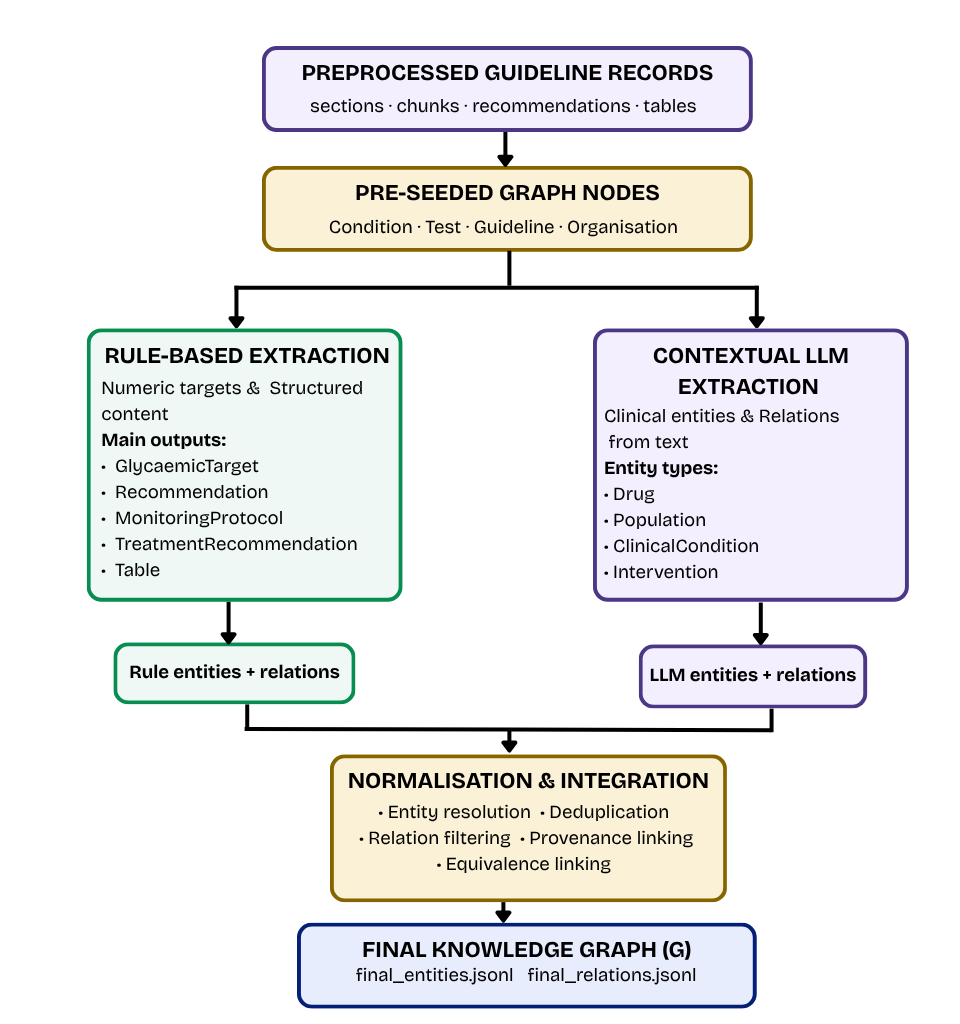
\includegraphics[width=\textwidth]{inc/figures/extraction_architecture.png}
    \caption{Layered extraction architecture}
    \label{fig:extraction}
\end{figure}

The output of both layers, the entity records in $\mathcal{V}$ and relation records in $\mathcal{R}$, passes to the normalisation stage, which resolves duplicates, converts units, and integrates both record sets into the finished graph $G$, described next in Section~\ref{sec:normalisation}.

\section{Normalisation and Graph Integration}
\label{sec:normalisation}

The normalisation stage takes the entity records $\mathcal{V}$ and relation records $\mathcal{R}$ produced by $\xi$ and integrates them into the unified graph $G$. It addresses three problems the extraction stage necessarily leaves unresolved --- entity duplication, terminological variation, and unit inconsistency. Entity deduplication is studied in the entity resolution and record linkage
literature \cite{getoor2012,christen2012,brizan2015}, and mapping biomedical
mentions to standard concepts is a long-standing task in clinical NLP, for
example for disease names \cite{singh2013}. Unit normalisation is needed here
because clinical measurements are reported on different scales across
guidelines \cite{hoelzel2004}. The contribution of this stage is applying both
steps within one multi-guideline pipeline.

The normalisation stage is formalised as a function
\begin{equation}
\eta: (\mathcal{V} \times \mathcal{R}) \rightarrow G
\label{eq:normalisation}
\end{equation}
where $G = (V, E, \mathcal{T}_V, \mathcal{T}_E, \phi, \psi, \lambda)$ is the graph defined in Section~\ref{sec:graph-model}. $\eta$ has to satisfy two properties. \textit{Provenance monotonicity}: merging two records never reduces the provenance carried by the result, since the provenance of the merged element is the union of everything that went into it.

\subsection{Entity Deduplication}
\label{sec:deduplication}

Both extraction layers can independently identify the same real-world entity from different passages of the same document, or from different documents entirely, producing more than one record for the same concept. Loading those duplicates into the graph without resolving them first would leave several near-identical nodes standing in for one entity, splitting relations that should converge on a single node across all of them and making cross-guideline queries incomplete.

Deduplication uses a type-specific equivalence relation $\sim_\tau$ over entity records. Two records $e_i, e_j$ of type $\tau$ count as duplicates exactly when $e_i \sim_\tau e_j$, and are then merged into one node whose provenance is the union of $\pi_{e_i}$ and $\pi_{e_j}$. This relation takes two different forms, depending on the structural properties of the type.

\paragraph{Name-bearing entity types.}
For types whose identity is a canonical name string --- \textsc{Drug}, \textsc{Condition}, \textsc{ClinicalCondition}, \textsc{Intervention}, and \textsc{Test} --- the equivalence relation is
$$e_i \sim_\tau e_j \iff \sigma(\text{name}(e_i)) = \sigma(\text{name}(e_j))$$
where $\sigma: \mathbb{S} \rightarrow \mathbb{S}$ normalises a surface form in three steps: it collapses whitespace and strips leading and trailing spaces, applies Unicode case folding, and then maps the result through a type-specific canonicalisation dictionary $\Delta_\tau: \mathbb{S} \rightarrow \mathbb{S}$ that resolves known surface-form variants to one canonical representative. In the implementation, separate alias mappings are used for different
name-bearing types, including tests, drugs, and clinical conditions.
For example, the test aliases \texttt{fpg},
\texttt{fasting plasma glucose}, and \texttt{fasting glucose} all
resolve to \texttt{FPG}. These dictionaries are fixed at schema design time and not updated while processing runs; any surface form not already in $\Delta_\tau$ is treated as a new entity, not a variant of an existing one. Because everything here is deterministic, $\sim_\tau$ is exactly reproducible --- the same input records and the same dictionary always produce the same deduplication output.

No similarity threshold or fuzzy string matching is applied in this
deduplication step. Deterministic matching is chosen over probabilistic matching because a fuzzy match that incorrectly merges two distinct drug or condition names would put an error into the graph that is hard to catch by inspection afterward. The trade-off is reduced recall, discussed in Chapter~\ref{chap:evaluation}.

\paragraph{Structured numerical entity types.}
For types whose identity comes from a combination of numerical and categorical fields, not a name string --- \textsc{GlycaemicTarget} and \textsc{MonitoringProtocol} --- the equivalence relation is defined over a composite key,
$$e_i \sim_\tau e_j \iff \kappa_\tau(e_i) = \kappa_\tau(e_j)$$
where $\kappa_\tau: \mathcal{E} \rightarrow \mathcal{K}_\tau$ projects a record onto its defining fields. For \textsc{GlycaemicTarget}, the key is
$$\kappa_{\textsc{GT}}(e) = (\text{metric}(e),\ \text{units}(e),\ \text{op}(e),\ \text{value}(e))$$
Two records are duplicates only if all four fields match exactly. As with the name-bearing types, no tolerance is applied anywhere in this comparison.

\paragraph{Scoping of deduplication.}
For global node types, the relation applies across the whole corpus. Two records from different guidelines that satisfy $\sim_\tau$ merge into one global node. For organisation-scoped types, deduplication stays within a single issuing organisation. Two \textsc{GlycaemicTarget} records from different organisations that happen to satisfy $\kappa_{\textsc{GT}}(e_i) = \kappa_{\textsc{GT}}(e_j)$ are not merged, because they represent two independent clinical positions that happen to agree numerically, not one shared statement. That agreement is instead expressed through an \textsc{equivalent\_to} edge, created during unit normalisation, described next.

\subsection{Unit Normalisation}
\label{sec:unit-normalisation}

As established in Section~\ref{sec:heterogeneity}, different organisations express the same clinical quantities in different units. Comparing numerical thresholds across guidelines only means anything once every value is expressed in one common unit system.

Clinical quantities such as HbA1c are reported on different scales across
guideline families, for example NGSP percent and IFCC mmol/mol, which are
related by a linear regression \cite{hoelzel2004}, so thresholds from
different sources have to be converted before they can be compared. This is
made easier by never merging organisation-scoped nodes during deduplication,
which keeps each guideline's own threshold as a distinct node that can be
compared against another's.

Unit normalisation is applied to \textsc{GlycaemicTarget} entities during integration. Plasma glucose values given in milligrams per decilitre convert to millimoles per litre by
$$\text{value}_{\text{mmol/L}} = \frac{\text{value}_{\text{mg/dL}}}{18.0}$$
where the divisor is the standard factor for converting plasma glucose between the two units. For example, a stored value of 126~mg/dL becomes
$126/18.0 = 7.0$~mmol/L. A target written as 126~mg/dL can therefore be
compared directly with a target written as 7.0~mmol/L once both are
represented through the normalised field. This factor is not asserted independently of the corpus; several guidelines state both units for the same threshold directly, for example the IDF criteria \cite{IDF2025} give FPG $<$6.1~mmol/L (110~mg/dL) for normal fasting glucose and FPG $\geq$7.0~mmol/L (126~mg/dL) for the diabetes diagnostic threshold, and a 2-hour post-load value of $<$10~mmol/L (180~mg/dL). Dividing each mg/dL figure by 18.016 reproduces the mmol/L figure given alongside it, confirming the pipeline's rounded divisor of 18.0 against the corpus's own stated equivalences rather than an external constant. The pipeline uses 18.0 rather than 18.016; for the threshold values present in this corpus the two give identical results once rounded to one decimal place. The original value and unit are kept as properties on the node alongside the normalised one, so the source document's original expression is never lost. Glycated haemoglobin appears in the corpus both as a percentage and in IFCC units (mmol/mol); both forms are retained, and each is converted to the other using the linear relation from the IFCC reference method \cite{hoelzel2004}:
$$\text{value}_{\text{mmol/mol}} = \frac{\text{value}_{\%} - 2.152}{0.09148}$$
As with plasma glucose, the source value and unit stay on the node alongside the converted one.

After unit normalisation, the implementation rounds the normalised plasma-glucose value to one decimal place before comparison. Two \textsc{GlycaemicTarget} nodes from different guidelines are considered equivalent if
\begin{align*}
e_i \equiv e_j \iff\ &\text{metric}(e_i) = \text{metric}(e_j)\ \wedge\ 
\text{op}(e_i) = \text{op}(e_j)\ \wedge\ \\
&\operatorname{round}_1\bigl(\text{value}_{\text{mmol/L}}(e_i)\bigr) = \operatorname{round}_1\bigl(\text{value}_{\text{mmol/L}}(e_j)\bigr)
\end{align*}

This requires exact equality of the rounded value, with no additional tolerance band. This is workable for the thresholds compared in this corpus because
values such as the fasting plasma glucose threshold of 7.0~mmol/L
resolve to the same rounded value after normalisation. For each pair $(e_i, e_j)$ satisfying these conditions and coming from different organisations, a directed \textsc{equivalent\_to} edge is created between them.

Conceptually, equivalence detection belongs to normalisation because it depends on normalised target values. In the implementation, the normalised plasma-glucose field and the corresponding \textsc{equivalent\_to} relations are computed while assembling the rule-derived target records, before the later global deduplication pass. This step is where the fourth contribution of the chapter is actually realised. No guideline states outright that its own threshold agrees with another organisation's; the relation is not extracted from text at all. It exists only because unit conversion makes independently stated thresholds directly comparable once they are expressed the same way. Normalisation is therefore not only a cleanup step; it is also the point in the pipeline that produces a class of cross-guideline relation that no single-guideline pipeline, and no extraction method working on raw text, could produce on its own.

\subsection{Layered Output Integration}
\label{sec:integration}

Merging records that refer to the same concept onto one canonical identifier follows the same principle used by controlled vocabulary resources in biomedicine \cite{bodenreider2004}.

The final step merges the deduplicated outputs of the rule-based and LLM-based layers into one set of nodes and edges. When the LLM layer produces an entity record, the entity-resolution step checks it against the index of canonical entities already established by the rule layer and the pre-seeded anchor nodes. If it finds a match under $\sim_\tau$, the LLM record is discarded and the canonical entity is referenced instead; only when no canonical match exists does the record keep an \texttt{llm\_} identifier prefix and get retained as a new entity. This applies the entity-resolution rule of $\mathcal{C}$ again at the integration stage, in addition to the prompt-level instruction already described in Section~\ref{sec:llm-extraction}.

Relations that resolve to the same source node, relation type, and destination node are deduplicated during integration; the implementation retains one relation record after rewiring rather than creating parallel duplicate edges. Relations present in only one layer's output are kept as they are. The two layers are meant to complement, not duplicate, each other, so a relation found only by the rule layer, or only by the LLM layer, is not treated as less valid for that reason.

The integrated, normalised, and deduplicated set of nodes and edges is then loaded into the graph database, producing the finished graph $G = (V, E, \mathcal{T}_V, \mathcal{T}_E, \phi, \psi, \lambda)$ as defined in Section~\ref{sec:graph-model}. Where an entity or relation is produced by an extraction component, its extraction-method metadata is retained so that rule-derived and language-model-derived records can be distinguished during analysis.

\section{Question Generation from the Knowledge Graph}
\label{sec:questions}

The final stage of the pipeline uses the finished graph $G$ as a controlled knowledge source for generating clinical questions. Two properties are both wanted here and are hard to get at the same time. Linguistic variety means that questions need not all use one fixed surface template for a given relation type. Factual grounding means every claim made in a question, or embedded in its answer, has to trace back to a specific assertion already in the graph.

A purely template-based approach, substituting graph values into fixed sentence
patterns, guarantees grounding but at a real cost to variety. Every question on
the same relation type sounds the same, which is likely to make the catalogue
predictable for a learner. Low diversity is also a recognised problem in
knowledge-base question generation more broadly \cite{bi2020}.
A purely generative approach, where a language model is simply prompted to
write questions about diabetes, gets the variety but brings back the
hallucination risk this chapter has already discussed. The model can produce a
question whose factual claim is not actually supported by the corpus, or
attribute a recommendation to the wrong organisation \cite{huang2025}. Language
models can be prompted with structured knowledge-base input to generate
questions \cite{liang2023}, and the hybrid design in this section builds on
that idea while splitting the two responsibilities between the component suited
to each. The graph decides what is asked, and the language model decides how it
is phrased.
\subsection*{The Question Generation Function}

Question generation is formalised as a function
\begin{equation}
\gamma: G \rightarrow \mathcal{Q}
\label{eq:qgen}
\end{equation}
mapping the graph to a catalogue of validated questions $\mathcal{Q}$. $\gamma$ is built from three sub-functions applied in order --- targeting, formulation, and validation --- with the anchor produced by targeting carried forward through formulation so that validation can compare the final question against it. The factual content of every question is fixed by the first sub-function, before the language model is ever called, and checked again by the third, after the model has produced its output. The model itself, in the middle step, has no access to the full graph. It receives only the selected anchor as factual input and is instructed not to introduce information beyond it.

\begin{figure}[!ht]
    \centering
    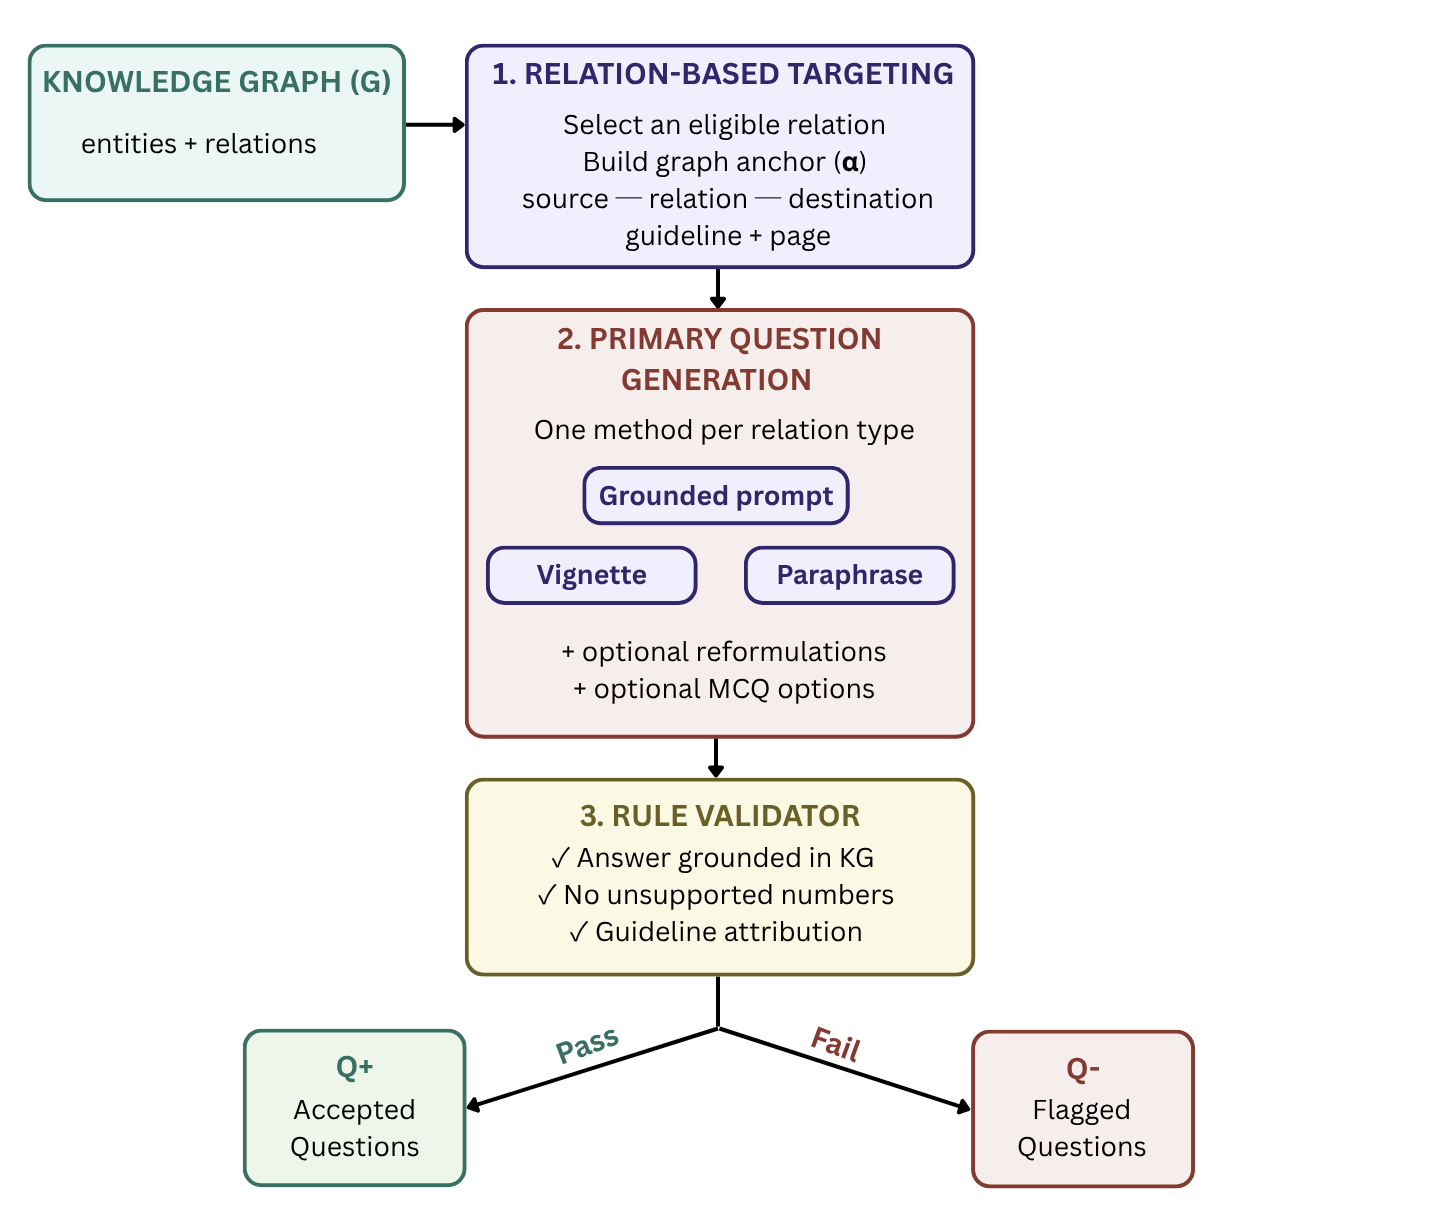
\includegraphics[width=\textwidth]{inc/figures/question_generation.png}
    \caption{Hybrid question generation pipeline.}
    \label{fig:questions}
\end{figure}

\subsection{Graph-Controlled Question Targeting}
\label{sec:targeting}

Generating questions from structured knowledge, not free text, is an established approach in question generation research \cite{guo2024,bi2020}.

The first sub-function does targeting entirely by rule-based traversal of the graph, with no language model involved.
$$\alpha: G \rightarrow \mathcal{A} \times \mathcal{D}_\gamma$$
For each edge selected, $\alpha$ produces two things. A graph anchor $a \in \mathcal{A}$ is a frozen record of the fact the question will test, carrying the source node, relation type, destination node, guideline, and page. For each selected edge, the implementation determines a question type and one primary generation method from fixed relation-based mappings. MCQ eligibility is also predefined for selected relation types, while the primary difficulty label is assigned according to the generation method

Question generation is restricted to a selected subset of graph relation types for which a meaningful question form is defined. The implementation maps each eligible relation type to a question type and generation method; for example, \textsc{first\_line\_for} maps to a \textit{which} question, \textsc{has\_target} to a \textit{what} question, \textsc{contraindicated\_in} to a \textit{yes/no} question, and \textsc{manages} to a scenario-based \textit{how} question. \textsc{equivalent\_to} edges are treated separately. They connect the same clinical concept across two guidelines, so questions derived from them test recall of one guideline's position and cross-guideline awareness at the same time.

The question taxonomy $\mathcal{T}_Q = \{\textsc{which}, \textsc{what}, \textsc{yes\_no}, \textsc{how}\}$ is decided entirely by the relation type of the anchor edge, not by the model. The mapping is a fixed lookup table set before any generation begins. \textsc{first\_line\_for} edges produce \textit{which} questions, \textsc{has\_target} edges produce \textit{what} questions, \textsc{contraindicated\_in} edges produce \textit{yes/no} questions, and \textsc{manages} edges produce scenario-based \textit{how} questions. The distribution of question types across the catalogue is a direct function of the graph's edge distribution, not of any generative choice made downstream.

\subsection{Language Model Question Formulation}
\label{sec:formulation}

The second sub-function uses a language model to produce the natural-language form of the question.
$$\beta: \mathcal{A} \times \mathcal{D}_\gamma \rightarrow \mathcal{Q}_{\text{raw}}$$
The model receives the anchor $a$ as its only factual input, given as a frozen context block, configured according to $\delta$. It is instructed not to introduce drug names, numerical values, targets, or guideline references that are absent from the anchor. In vignette-style formulations it may additionally describe the patient and symptoms in words; such details are not drawn from the anchor, and the validator checks them only for numerical values. Its intended role is therefore linguistic transformation: it may vary sentence structure, framing, and formality while preserving the factual assertion represented by the anchor.

This is a tighter version of the same constraint used during extraction. In extraction, the model was confined to a predefined schema of types and canonical names. Here, it is confined further, to the single factual assertion in one anchor. The same principle runs through both stages. Its intended role is to classify or rephrase information supplied through the structured input rather than to introduce additional clinical content.

For each anchor, the method assigned to its relation type determines how the
question is generated. The three generation methods are a graph-grounded
prompt, a clinical vignette, and a template paraphrase. For the grounded-prompt
method, the model generates one primary question, and difficulty variants may
be stored alongside it as reformulations within the same record. Each selected
anchor produces at most one primary question record in the catalogue, and exact
duplicate question texts are skipped. For relation types that support it, the
model also generates multiple-choice distractors. The correct answer is fixed
by the anchor and is never generated. For eligible multiple-choice questions,
the model is given a candidate pool sampled from real \textsc{Drug} nodes in
the graph and instructed to choose plausible distractors from that pool. This
differs from distractor generation from free text, as in \cite{gao2019}, where
distractors are generated from the passage rather than drawn from a set of
known entities. The returned strings are not programmatically checked against
the pool.

\subsection{Rule-Based Validation}
\label{sec:validation}

Language models can produce text that reads fluently but is not actually supported by their input \cite{huang2025}, so every generated question is checked against its anchor before it enters the catalogue.
$$\nu: \mathcal{Q}_{\text{raw}} \times \mathcal{A} \rightarrow \{0, 1\} \times \mathcal{Q}$$
The validator applies three checks, each comparing the generated question text against the frozen anchor.

The first check is answer-key consistency. For questions whose answer is an entity, the validator confirms that the answer named in the anchor is actually a node in the graph. For questions derived from \textsc{has\_target} edges, where the answer is a numerical threshold and not an entity name, it confirms that the number in the answer matches the property values of the destination node $v_d$ in the anchor.

The second check is hallucinated number detection. Any number in the generated question that does not appear in the anchor is flagged as a possible hallucination. This matters most for scenario-based questions, where the model can be tempted to invent realistic-sounding patient details, ages, lab values, or disease duration, that are not grounded in the anchor at all.

The third check detects conflicting guideline attribution. If the relation is associated with one of the recognised organisations, the validator rejects a question that explicitly names a different organisation. A question that credits a recommendation to the wrong organisation is factually wrong even if the recommendation content itself is stated correctly.

Questions passing all three checks go into the validated catalogue $\mathcal{Q}^+$, with anchor, generation configuration, difficulty level, and validation status recorded as metadata. Questions failing one or more checks go into a separate flagged catalogue $\mathcal{Q}^-$ for manual review. They are not discarded, since a failed check can just as easily mean the rule was too conservative as mean there is a genuine factual error. This trades some precision for recall, at the cost of needing human review on the borderline cases, which is a reasonable trade-off given that a wrong clinical claim in the catalogue actually matters. The validator checks whether the fluency and variety introduced by the language model in $\beta$ remain consistent with the content represented by the anchor in $\alpha$. What the validator checks is consistency with the anchor, not clinical correctness. A question built on an incorrect graph edge will pass all three checks, since the checks compare the question against the anchor, not against the source guideline. Chapter~\ref{chap:evaluation} reports how often this occurred in practice.

\paragraph{Worked example}
Consider an anchor in which a \textsc{Condition} node is linked by \textsc{has\_target} to a \textsc{GlycaemicTarget} representing FPG $\geq 7.0$~mmol/L. The relation also retains the organisation and page metadata associated with the extracted assertion where available. The targeting function $\alpha$ selects this relation and freezes its source node, relation type, destination node, and provenance as the anchor. The formulation function $\beta$
receives only this anchor and turns it into a question such as
``What fasting plasma glucose threshold does this guideline specify?''
The answer remains 7.0~mmol/L because it comes from the destination node,
not from the language model. The validator $\nu$ then checks the generated
question and answer against the same anchor. If the question instead
introduced a threshold of 8.0~mmol/L, the numerical check would flag it.

Figure~\ref{fig:questions} shows how the design keeps these two responsibilities separate. The left-hand annotations show the fixed mapping from relation type to question type, decided entirely by the rule engine with no language model involvement. The right-hand annotations show the range of linguistically distinct question variants the model generates from a single anchor, none of which may go beyond what the anchor specifies. The validator at the foot of the pipeline checks the generated output
against the original anchor using the three rules described above.

The composition is expressed as $(a,\delta) = \alpha(G)$, $q_{\text{raw}} = \beta(a,\delta)$, and $q = \nu(q_{\text{raw}}, a)$, making explicit that the validator $\nu$ consumes both the formulated question and the original anchor. This composed pipeline is the third contribution of this chapter. It represents question generation anchored
to the graph while keeping the factual content fixed by the selected
anchor. The factual content of each question comes from the graph in
$\alpha$. The language model in $\beta$ turns this content into natural
language, and the validator in $\nu$ checks the generated question against
the original graph assertion. The answer-bearing relation therefore remains
fixed by the anchor throughout generation. The language model contributes
the wording of the question and, where applicable, the distractor options
selected from the permitted candidate pool. This separation allows the
pipeline to produce questions with varied wording while keeping them tied
to a specific graph assertion. The concrete results of applying $\gamma$
to the graph, including question counts, type distributions, and validation
outcomes, are reported in Chapter~\ref{chap:evaluation}.


 \chapter{Experimental Evaluation}
\label{chap:evaluation}

This chapter instantiates the framework defined in
Chapter~\ref{chap:construction} on a corpus of Type 1 and Type 2 diabetes guidelines.
Chapter~\ref{chap:construction} defined a four-stage architecture together with
the schema, extraction rules, and normalisation procedures configured for the
diabetes guideline corpus;
this chapter is the diabetes-specific instantiation and owns all concrete
details: corpus composition, tool choices, implementation decisions,
quantitative outcomes, and an analysis of where the pipeline succeeded and
where it did not. The sections follow the pipeline stages: corpus
selection~(Section~\ref{sec:exp_data}), document ingestion and
preprocessing~(Section~\ref{sec:exp_ingestion}), knowledge graph
construction~(Section~\ref{sec:exp_norm}), question
generation~(Section~\ref{sec:exp_questions}), evaluation of the question
catalogue~(Section~\ref{sec:exp_quality}), and
limitations~(Section~\ref{sec:exp_limitations}).

\section{Data Sources and Corpus}
\label{sec:exp_data}

The corpus is drawn from four guideline-producing organisations: the
American Diabetes Association~(ADA)\footnote{https://www.diabetes.org/}, the National Institute for Health and
Care Excellence~(NICE)\footnote{https://www.nice.org.uk/}, the International Diabetes Federation~(IDF)\footnote{https://www.idf.org/}, and
Diabetes Canada\footnote{https://www.diabetes.ca/}. Together they satisfy the four selection criteria defined
in Section~\ref{sec:corpus}. The corpus comprises eight documents, each
processed as one ingestion unit. Table~\ref{tab:corpus} reports the
structural properties measured at the output of the ingestion stage.
The IDF document served as the initial development document for the
extraction pipeline before the implementation was extended to the other
three guideline families.

\begin{table}[!ht]
\centering
\small\setlength{\tabcolsep}{5pt}
\begin{tabular}{p{2.1cm} p{5.2cm} r r r r p{2.0cm}}
\hline
\textbf{Organisation} & \textbf{Document} & \textbf{Year} & \textbf{Pp.}
                      & \textbf{Rec.} & \textbf{Tab.} & \textbf{Units} \\
\hline
ADA
  & Standards of Care in Diabetes
  & 2026 & 377 & 176 & 113 & mg/dL \\[2pt]
NICE
  & NG17: Type~1 Diabetes in Adults
  & 2026 &  64 & 100 &   0 & mmol/L, \newline mmol/mol \\[2pt]
NICE
  & NG28: Type~2 Diabetes in Adults
  & 2026 & 124 & 116 &   0 & mmol/L, \newline mmol/mol \\[2pt]
IDF
  & Global Clinical Practice Recommendations
  & 2025 & 112 &   10 &  21 & mmol/L \\[2pt]
Diabetes Canada
  & CPG 2018, Chapter~3
  & 2018 &   6 &  2 &  5 & mmol/L \\[2pt]
Diabetes Canada
  & CPG 2018, Chapter~4
  & 2018 &   4 &  2 &   1 & mmol/L \\[2pt]
Diabetes Canada
  & CPG 2018, Chapter~8
  & 2018 &   5 &  5 &  1 & mmol/L \\[2pt]
Diabetes Canada
  & CPG 2018, Chapter~9
  & 2018 &   7 &  8 &   1 & mmol/L \\[2pt]
\hline
\textbf{Total}
  & \textit{8 documents, 4 organisations}
  & & \textbf{699} & \textbf{419} & \textbf{142} & \\
\hline
\end{tabular}
\caption{Corpus documents and structural properties.}
\label{tab:corpus}
\end{table}

\subsection{Corpus against Selection Criteria}
\label{sec:corpus-criteria}

\paragraph{Geographic and systemic diversity.}
The four organisations publish from different national and international
contexts: the ADA in the United States, NICE in England and Wales, Diabetes
Canada in Canada, and the IDF as an international federation. Selecting
organisations from more than one context gives variation in guideline origin,
publishing convention, and recommendation structure, rather than restricting
the corpus to a single publisher.

\paragraph{Clinical coverage.}
Across the eight documents the corpus addresses all five clinical domains
identified in Section~\ref{sec:corpus}: diagnosis and classification~(ADA
Table~2.1, Canada Ch.~3), screening~(NICE NG17 Section~1.1, Canada Ch.~3),
glycaemic targets~(all four organisations), pharmacological management~(ADA
Section~9, NICE NG28, IDF, Canada Ch.~8--9), and monitoring~(NICE NG17
Section~1.5, Canada Ch.~4). No domain is covered by a single organisation only.

\paragraph{Format diversity.}
NICE documents present recommendations as numbered statements, and convey
their strength through wording rather than a grade label. In the versions
processed here, the NICE guidelines contained [N] embedded tables. The ADA
document combines numbered recommendations, each with an evidence grade, with
113 embedded tables in a three-column page layout. The IDF uses prose and two-column
care-tier tables with no structured recommendation numbering. The Canada
chapters are journal articles with graded recommendations embedded in
continuous clinical commentary.

\paragraph{Recommendation specificity.}
All documents contain actionable recommendations specifying drug choices,
numerical targets, or monitoring schedules. High-level policy documents were
excluded because they do not produce meaningful pharmacological or measurement
entities in the schema.

\subsection{Structural Heterogeneity in Practice}
\label{sec:heterogeneity-practice}

NICE contributes 496 chunks, 216 structured recommendations across its two documents and
zero tables; the ADA contributes 1,832 prose chunks, 176 structured
recommendation elements, and 113 reconstructed tables; the IDF
contributes 10 recommendation elements and 21 tables; the Canada chapters
contributes 107 chunks, 8 tables and 17 recommendations. The measurement unit column illustrates the
unit inconsistency: the ADA uses mg/dL for plasma glucose while the other
three use mmol/L, and NICE reports HbA1c in mmol/mol rather than as a
percentage. These three dimensions of heterogeneity directly shaped every
design decision in the ingestion and extraction stages.

Figure~\ref{fig:corpus} shows the number of chunks, recommendations, tables,
and sections extracted per organisation, visualising the same structural
volume reported in Table~\ref{tab:ingestion} and highlighting NICE's absence
of tables and the ADA's dominance in chunk and table count..

\begin{figure}[!ht]
    \centering
    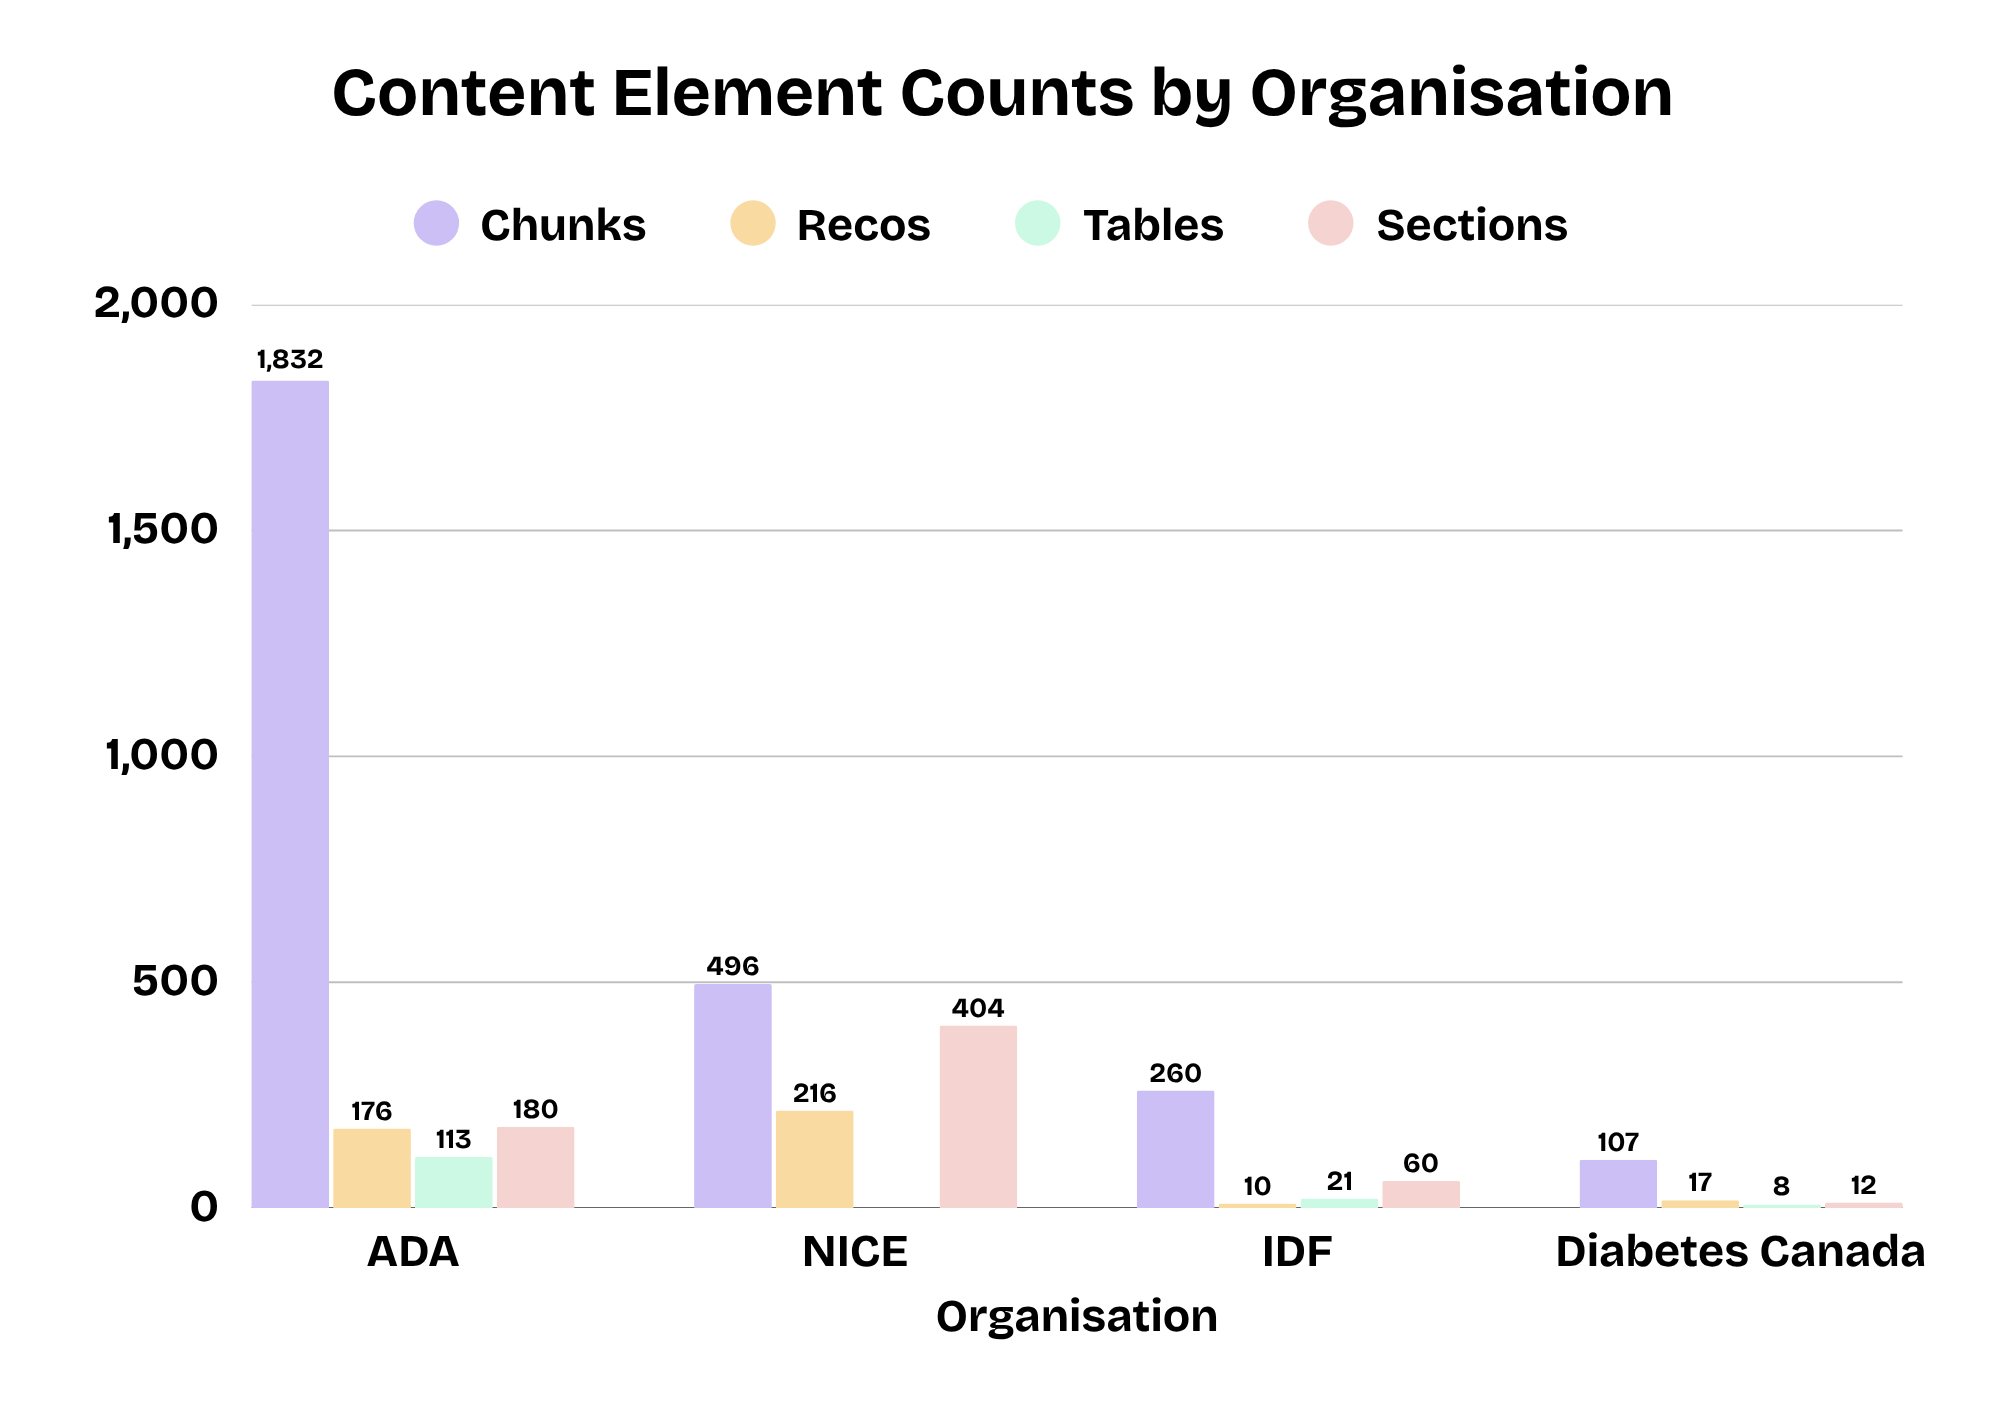
\includegraphics[width=\textwidth]{inc/figures/corpus.png}
    \caption{Structural profile of the guideline corpus by organisation.}
    \label{fig:corpus}
\end{figure}

\section{Document Ingestion and Preprocessing}
\label{sec:exp_ingestion}

The ingestion stage applies $\varphi: \mathcal{D} \rightarrow 2^{\mathcal{E}}$
to each of the eight corpus documents. This section describes the parsing
tool, the document-family-specific text repairs required before extraction
could begin, and the resulting element counts.

\subsection{Document Parsing Tool}
\label{sec:exp_parsing}

The ingestion pipeline uses PyMuPDF~\cite{pymupdf2026}\footnote{PyMuPDF,
version 1.28.0, \url{https://pymupdf.readthedocs.io}.} (via the
\texttt{fitz} interface) as its primary PDF extraction engine and
\texttt{pdfplumber}~\cite{yang2025}\footnote{pdfplumber, version 0.11.10,
\url{https://github.com/jsvine/pdfplumber}.} for table extraction.
Docling~\cite{auer2024}\footnote{Docling, version 2.130.0,
\url{https://github.com/docling-project/docling}.} is retained in the ingestion
script as an optional conversion step, but it was not adopted. Its output is not
used by the downstream stages, and the element records are unchanged when it is
unavailable. On five pages of one Diabetes Canada chapter, block extraction with
PyMuPDF took 0.03 seconds and table extraction with pdfplumber 0.89 seconds (mean
of five runs), against 114 seconds for a Docling conversion of the same pages on
the development laptop (CPU only),\footnote{CPU 1.70 GHz, 12 cores; RAM 16GB; Intel UHD Graphics.} The text export
requested by the script also carries no page numbers or coordinates. Every element
record needs a page range, and reading order and heading recovery need block
coordinates, so the element records are built from PyMuPDF blocks and pdfplumber
tables. No systematic comparison of the parsers was carried out.

PDF extraction from scientific documents introduces known artefacts,
including ligature encoding, token-boundary errors, and multi-column layout
bleed~\cite{bast2017}. PyMuPDF is the base of the pipeline because several
corpus-specific steps need direct access to raw text blocks with page
identifiers, font sizes, and bounding boxes. Reading order and heading
recovery use the block coordinates and font sizes, and the ADA and IDF
recommendation extractors work on the ordered raw blocks rather than on merged
section text. A repair for concatenated words, written for the Diabetes Canada
PDFs, is applied to every extracted block and to the table cells of
journal-style documents. Tables are reconstructed with \texttt{pdfplumber}.

The output for each document is a set of typed JSONL files:
\texttt{chunks.jsonl} for \textsc{Prose} elements,
\texttt{recommendations.jsonl} for \textsc{Recommendation} elements, a
\texttt{tables/} directory of CSV files for \textsc{Table} elements, and
\texttt{sections.jsonl} for \textsc{Section} elements. These constitute
the intermediate representation consumed by the extraction stage.

\subsection{Text Repair Passes}
\label{sec:exp_repair}

The ingestion implementation contains several document-family-specific
repairs and extraction rules that were added after inspecting failures in
the raw PDF output. Table~\ref{tab:repair} summarises the ones that directly
affected the corpus representation used here.

\begin{table}[!ht]
\centering
\small\setlength{\tabcolsep}{5pt}
\begin{tabular}{p{0.7cm} p{3.2cm} p{2.5cm} p{4.8cm}}
\hline
\textbf{Fix} & \textbf{Artefact} & \textbf{Affected families}
              & \textbf{Repair operation} \\
\hline
A & Word concatenation and camelCase runs
    (e.g.\ \texttt{Ageofonset}, \texttt{Type1diabetes})
  & Diabetes Canada
  & Split at digit--letter and camelCase boundaries when
    concatenation density exceeds a threshold \\[4pt]
B & Canada numbered recommendations parsed as prose
    (\texttt{"1. Diabetes should..."})
  & Diabetes Canada
  & Dedicated regex \texttt{CANADA\_RECO\_RE} promotes
    matched blocks to \textsc{Recommendation} elements \\[4pt]
C & ADA boxed recommendation text fused into single spans by PyMuPDF
  & ADA
  & Separate extractor \texttt{extract\_ada\_recommendation\_blocks}
    runs on raw blocks before section merge \\[4pt]
D & NICE table captions consumed as section headings
  & NICE
  & \texttt{looks\_like\_heading()} short-circuits on
    \texttt{NICE\_TABLEISH\_RE} matches when NICE numbering
    is active \\[4pt]
E & IDF ``Optimal / Basic / Recommended Care'' prose blocks
    not matched as recommendations
  & IDF
  & \texttt{extract\_idf\_recommendations()} with pattern
    \texttt{IDF\_CARE\_RE} promotes matching blocks \\[4pt]
F & Duplicate section headings or repeated heading blocks in the extracted page content
  & ADA, NICE, IDF
  & Per-page deduplication by title string in
    \texttt{recover\_headings()} \\[4pt]
\hline
\end{tabular}
\caption{Document-family-specific text repair passes.}
\label{tab:repair}
\end{table}

Fix~A is the most structurally significant for the Canada documents. The
\textit{Canadian Journal of Diabetes} typesetting pipeline produces PDF text
streams in which word boundaries are not encoded as whitespace: the string
\texttt{Ageofonset} must be reconstructed as \texttt{Age of onset} before
any pattern matching is possible. The repair applies unconditional digit--letter
splitting followed by conditional camelCase splitting when the density of
lowercase--uppercase transitions in a block exceeds 4\%.

Fix~C and Fix~D reflect the two most common extraction failures during
development: ADA clinical directives were being silently swallowed into
prose chunks, and NICE table captions were being misclassified as section
headings, producing spurious \textsc{Section} elements at the start of
tabular content.

No character- or token-level repairs were required for the IDF body text, whose Unicode streams are clean. Fix E instead addresses structural recognition of care-tier recommendation blocks.

\subsection{Ingestion Statistics}
\label{sec:exp_ingestion-stats}

Table~\ref{tab:ingestion} reports element counts after all repairs: the corpus
produces 2,695 chunks, 419 recommendation elements, and 142 tables, dominated by
the ADA document at 1,832 chunks and 176 recommendations, while the four Diabetes
Canada chapters, each covering only a few pages, contribute the fewest elements
individually. The 3,256 extracted content records represented by chunks,
recommendations, and tables form the principal inputs used by the downstream
extraction stages; the 656 section elements are consumed internally for
provenance annotation and are not passed forward.

\begin{table}[!ht]
\centering
\small
\begin{tabular}{llrrrr}
\hline
\textbf{Org.} & \textbf{Document} & \textbf{Chunks}
              & \textbf{Recos} & \textbf{Tables} & \textbf{Sections} \\
\hline
ADA          & Standards of Care 2026   & 1{,}832 & 176 & 113 & 180 \\
NICE         & NG17: Type~1 Diabetes    &   190   & 100 &   0 & 167 \\
NICE         & NG28: Type~2 Diabetes    &   306   & 116 &   0 & 237 \\
IDF          & Global CPR 2025          &   260   &   10 &  21 &  60 \\
Diab. Canada & CPG 2018 Ch.~3           &    30   &  2 &  5 &   3 \\
Diab. Canada & CPG 2018 Ch.~4           &    19   &  2 &   1 &   3 \\
Diab. Canada & CPG 2018 Ch.~8           &    23   &  5 &   1 &   3 \\
Diab. Canada & CPG 2018 Ch.~9           &    35   &  8 &   1 &   3 \\
\hline
\textbf{Total} &                        & 2{,}695 & 419 & 142 & 656 \\
\hline
\end{tabular}
\caption{Content-element counts after preprocessing.}
\label{tab:ingestion}
\end{table}

The ADA produces the largest chunk count (1,832) because its clinical directives are embedded in 377 pages of dense prose alongside structured recommendation elements. The Canada chapters produce relatively small chunk and recommendation sets because each chapter is short, but both prose chunks and explicitly extracted recommendation elements remain present in the intermediate representation. 
The IDF produces 10 recommendation elements through its dedicated care-level recommendation extractor, alongside 21 reconstructed tables.



\section{Knowledge Graph Construction}
\label{sec:exp_norm}

This section describes how the 3,256 content elements were converted into the
final Knowledge Graph $G$, covering entity and relation extraction, graph
database selection, entity deduplication, unit normalisation, cross-guideline
equivalence edges, and the resulting graph statistics.
\subsection{Entity and Relation Extraction}
\label{sec:extraction-impl}

Extraction is implemented as two scripts that follow the split defined in
Chapter~\ref{chap:construction}. Extraction-derived entities carry an \texttt{extract\_method} field where applicable.

\paragraph{Rule-based extraction.}
The rule extractor runs six passes in a fixed order. It first creates the
\textsc{Guideline} and \textsc{Organisation} nodes and the five canonical
\textsc{Condition} nodes. It then extracts \textsc{Recommendation} nodes from the
numbered recommendation records produced during ingestion, numerical targets from
chunk text, and table-derived nodes from the reconstructed tables. The last pass
creates the \textsc{equivalent\_to} relations once all documents have been
processed. The final graph contains 70 nodes labelled \texttt{rule}: 46
\textsc{GlycaemicTarget}, 14 \textsc{MonitoringProtocol} and 10
\textsc{TreatmentRecommendation}. A further 491 nodes are created by the same
script without a method label: 330 \textsc{Recommendation}, 139 \textsc{Table},
8 \textsc{Guideline}, 4 \textsc{Organisation}, and 5 each of \textsc{Condition}
and \textsc{Test}. A numerical target is linked to Type~1 or Type~2 diabetes only
when the surrounding text names exactly one of them.

\paragraph{Contextual extraction.}
The contextual extractor sends text chunks to a language model together with the
schema prompt shown in Appendix~\ref{app:extraction-prompts}. The reported graph
was produced with [[gpt-4o-mini through the OpenAI API]]\footnote{Model
identifier \texttt{gpt-4o-mini}, accessed through the OpenAI API,
\url{https://platform.openai.com/docs/models}.}, using
temperature~0 and a JSON response format. For each page, the prompt also contains
up to 20 facts already found by the rule extractor (numerical targets and short
recommendation summaries) as known context. The parser reads the JSON response but
does not check returned types against the schema. In the raw output, all 2,275
entities use declared types, but 2 of the 1,533 relations use undeclared types
(\textsc{researching} and \textsc{intervention}, one each); neither is part of the
final graph. Deduplication reduces the 2,275 entities to 1,942: \textsc{Drug} 627
to 438, \textsc{ClinicalCondition} 574 to 462 and \textsc{Intervention} 337 to 305,
while \textsc{Population} stays at 737. All 1,942 carry the same confidence value
of 0.7, so this field does not separate easy from hard extractions.


\subsection{Graph Database}
\label{sec:graph-db}

The Knowledge Graph is stored in Neo4j ~\cite{barrasa2023}\footnote{Neo4j [2026.04.0], \url{https://neo4j.com}.}
. Neo4j was chosen because it
stores both nodes and edges as first-class objects with arbitrary key-value
properties, which directly instantiates the property function
$\lambda: V \cup E \rightarrow 2^{\mathcal{P}}$. Provenance information such as the issuing organisation and source page
is stored directly on relations where it is available, without requiring
separate provenance nodes. Neo4j's Cypher query language also allows the
cross-guideline queries that motivate the graph to be expressed directly
as graph patterns. For example, the question \textit{which drugs are
recommended as first-line therapy by more than one organisation?} can be
answered by matching \textsc{first\_line\_for} relations and grouping the
results by organisation.

\subsection{Entity Deduplication}
\label{sec:dedup}

Deduplication applies the type-specific equivalence relation $\sim_\tau$
defined in Section~\ref{sec:normalisation} with two strategies.

For global node types (\textsc{Drug}, \textsc{Condition},
\textsc{ClinicalCondition}, \textsc{Intervention}, \textsc{Test}), two
records are equivalent when their normalised names satisfy
$\sigma(\text{name}_i) = \sigma(\text{name}_j)$, where $\sigma$ applies whitespace normalisation, lower-casing,
and type-specific synonym resolution. The implementation uses separate
alias mappings for tests, drugs, and clinical conditions. Representative entries are shown in Table~\ref{tab:synonyms}, which maps surface
forms such as \texttt{fpg} and \texttt{fasting plasma glucose} to the canonical
term \texttt{FPG}, and similarly collapses variant spellings of HbA1c and OGTT
into single canonical entities.

Deduplication of this kind is studied in the entity resolution
literature~\cite{getoor2012,christen2012}. Clinical concept
normalisation draws on the same principle as controlled vocabulary
resources such as the UMLS~\cite{bodenreider2004} and
RxNorm~\cite{hanna2013}, which map surface forms to canonical
identifiers; the synonym dictionary $\Delta$ plays an analogous
role within the scope of the corpus.

\begin{table}[!ht]
\centering
\small
\setlength{\tabcolsep}{6pt}

\begin{tabular}{p{0.68\textwidth} p{0.22\textwidth}}
\hline
\textbf{Surface form} & \textbf{Canonical form} \\
\hline

\texttt{fpg}, \texttt{fasting plasma glucose}, \texttt{fasting glucose}
&
\texttt{FPG}
\\[2pt]

\texttt{hba1c}, \texttt{a1c}, \texttt{glycated haemoglobin}
&
\texttt{HbA1c}
\\[2pt]

\texttt{ogtt}, \texttt{2h ogtt}, \texttt{2-h ogtt},
\texttt{75g ogtt}
&
\texttt{2h-OGTT}
\\

\hline
\end{tabular}
\caption{Selected synonym mappings for entity deduplication.}
\label{tab:synonyms}
\end{table}

Organisation-specific entities retain their source scope and use type-specific
identity keys rather than one common deduplication rule.
\textsc{GlycaemicTarget} records are keyed by metric, unit, comparison
operator, and value. \textsc{Recommendation} records use their recommendation
label and text, while \textsc{Table} and \textsc{MonitoringProtocol} records
use identifiers derived from the corresponding table or monitoring source. Records from different organisations are kept separate. For \textsc{GlycaemicTarget} records specifically, matching normalised thresholds across organisations are represented by an \textsc{equivalent\_to} edge as described below. 

\subsection{Unit Normalisation and Cross-Guideline Equivalence Edges}
\label{sec:unit-norm}

All plasma glucose threshold values are normalised to mmol/L using:

$$\text{value}_{\text{mmol/L}} = \frac{\text{value}_{\text{mg/dL}}}{18.0}$$

The divisor $18.0$ is the standard factor for converting plasma glucose
between mg/dL and mmol/L. The pipeline's corpus values confirm this:
the ADA states 126~mg/dL alongside $\geq 7.0$~mmol/L, and 200~mg/dL
alongside $\geq 11.1$~mmol/L,~\cite{ADA2026} both consistent with the divisor. The conversion is implemented in the shared helper
function \texttt{mgdl\_to\_mmolL}, imported by the rule extraction
script. HbA1c values are retained in their source unit, and the equivalent value on
the alternate scale is stored alongside it using the IFCC reference
relation~\cite{hoelzel2004}. Percentage values are converted to mmol/mol and mmol/mol values to
percentage, and the alternate representation is stored on the target node.
The current cross-guideline equivalence procedure, however, is restricted
to plasma-glucose targets represented in mmol/L.

\textsc{equivalent\_to} edges are created inside the rule extraction stage, after all documents
have been processed. The function \texttt{add\_cross\_guideline\_equivalences}
groups all \textsc{GlycaemicTarget} nodes by the tuple
$(\text{metric},\ \text{op},\ \text{round}(\text{value\_mmol\_L}, 1))$ and
adds directed \textsc{equivalent\_to} edges between matching target nodes
from different organisations within each group. The equivalence
check is exact equality on the rounded normalised value; no tolerance band
was applied. Although this operation is implemented in the rule-extraction
module, it runs only after the corpus-wide target extraction and numerical
normalisation pass; conceptually it therefore corresponds to the
normalisation stage defined in Chapter~\ref{chap:construction}.

Table~\ref{tab:equiv} lists the eight edges this process produced: three
organisations agree on an FPG threshold of 7.0 mmol/L, the same three agree
on a 2h-OGTT threshold of 11.1 mmol/L, and two further edges connect a Random
PG and a lower FPG bound between single pairs of organisations.

\begin{table}[!ht]
\centering
\small\setlength{\tabcolsep}{6pt}
\begin{tabular}{p{2.8cm} c p{2.4cm} p{2.4cm} p{2.4cm}}
\hline
\textbf{Metric} & \textbf{Op.} & \textbf{Value} & \textbf{Org. A}
                & \textbf{Org. B} \\
\hline
FPG          & $\geq$ & 7.0 mmol/L  & ADA            & Diabetes Canada \\
FPG          & $\geq$ & 7.0 mmol/L  & ADA            & IDF             \\
FPG          & $\geq$ & 7.0 mmol/L  & Diabetes Canada & IDF            \\
2h-OGTT      & $\geq$ & 11.1 mmol/L & ADA            & Diabetes Canada \\
2h-OGTT      & $\geq$ & 11.1 mmol/L & ADA            & IDF             \\
2h-OGTT      & $\geq$ & 11.1 mmol/L & Diabetes Canada & IDF            \\
Random PG    & $\geq$ & 11.1 mmol/L & ADA            & Diabetes Canada \\
FPG          & $<$    & 5.6 mmol/L  & ADA            & IDF             \\
\hline
\end{tabular}
\caption{Cross-guideline \texttt{equivalent\_to} edges after unit normalisation.}
\label{tab:equiv}
\end{table}

All eight edges concern diagnostic glucose thresholds, seven expressed as a
lower bound (\(\geq\)) and one as an upper bound for the normal range
(\(<5.6\)~mmol/L). The three FPG $\geq 7.0$~mmol/L edges form a triangle
across ADA, IDF, and Diabetes Canada; under the implemented equivalence
criterion their corresponding target nodes fall into the same normalised
group. No NICE plasma-glucose target nodes in the corpus satisfy the
implemented equivalence grouping.

Figure~\ref{fig:equiv} shows the eight edges as a matrix grouped by threshold,
making visible the two three-way agreements (FPG and 2h-OGTT) against the two
single-pair edges (Random PG and the normal-range FPG bound), and the absence
of NICE from every row.

\begin{figure}[!ht]
    \centering
    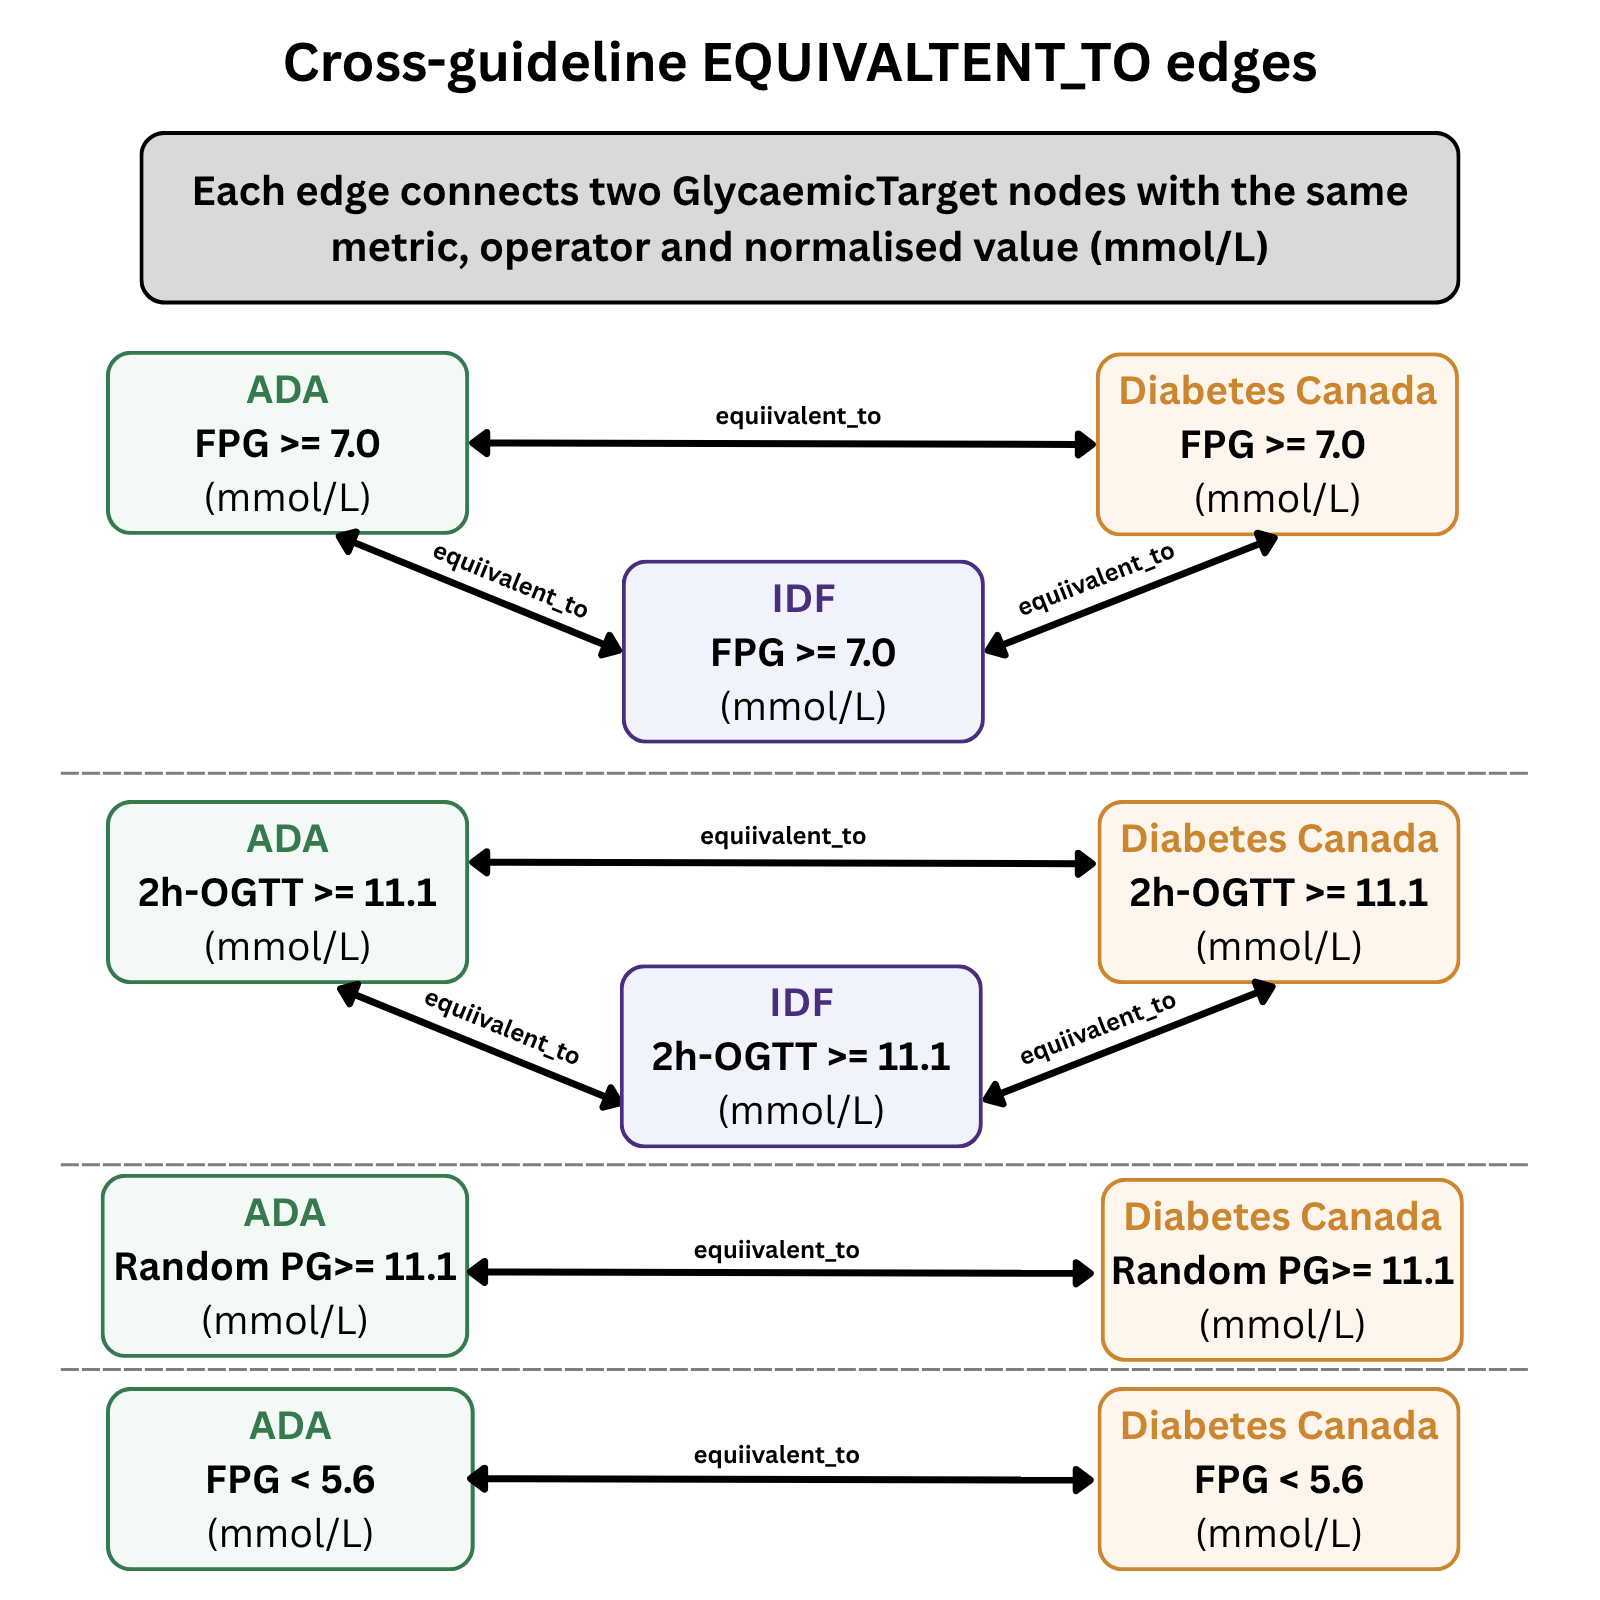
\includegraphics[width=0.85\textwidth]{inc/figures/equiv.png}
    \caption{Cross-guideline equivalence edges by diagnostic threshold.}
    \label{fig:equiv}
\end{figure}


\subsection{Final Graph Statistics}
\label{sec:graph-stats}

Tables~\ref{tab:nodes} and~\ref{tab:relations} report the composition of the
final Knowledge Graph after normalisation: 2,503 nodes across 13 types and 3,485
relations across 18 types, with \textsc{ClinicalCondition} and \textsc{Drug} the
largest node types and \textsc{mentioned\_in} the largest relation type at 1,409
edges. Figure~\ref{fig:graph-stats} shows how these node counts distribute across
the three scoping levels: global, organisation-scoped, and structural.


\begin{figure}[!ht]
    \centering
    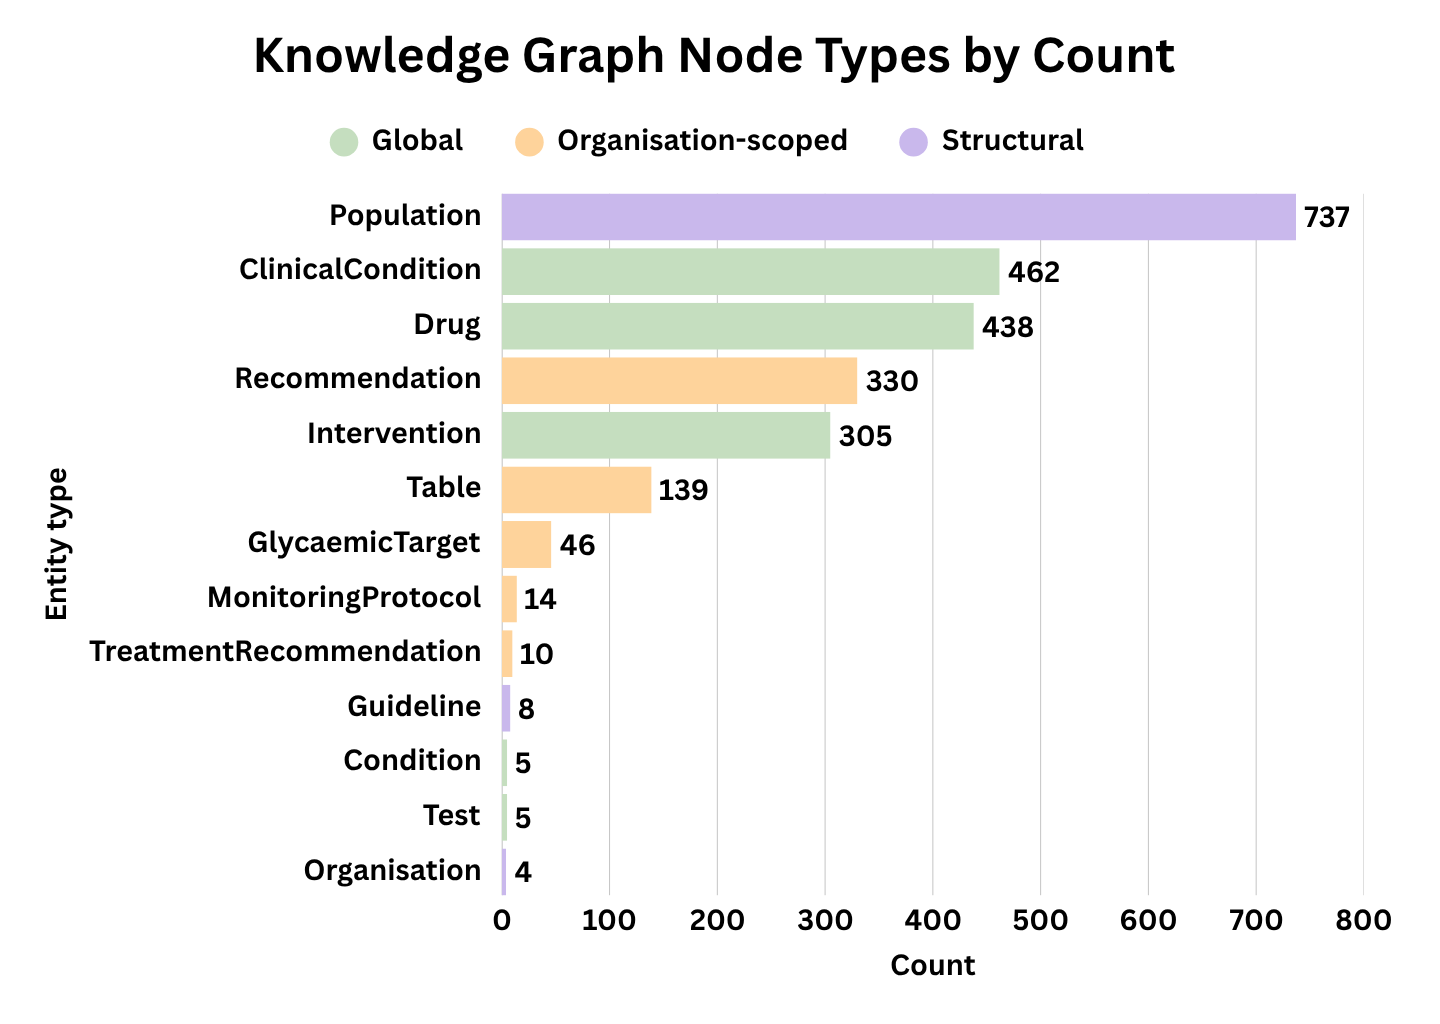
\includegraphics[width=\textwidth]{inc/figures/graph_stats.png}
    \caption{Node-type distribution by scoping level.}
    \label{fig:graph-stats}
\end{figure}

\begin{table}[!ht]
\centering
\small\setlength{\tabcolsep}{8pt}
\begin{tabular}{llr}
\hline
\textbf{Scoping level} & \textbf{Node type} & \textbf{Count} \\
\hline
Global
  & \textsc{Drug}                    & 438 \\
  & \textsc{ClinicalCondition}       & 462 \\
  & \textsc{Intervention}            & 305 \\
  & \textsc{Condition}               &   5 \\
  & \textsc{Test}                    &   5 \\
Organisation-scoped
  & \textsc{Recommendation}          & 330 \\
  & \textsc{Table}                   & 139 \\
  & \textsc{GlycaemicTarget}         &  46 \\
  & \textsc{MonitoringProtocol}      &  14 \\
  & \textsc{TreatmentRecommendation} &  10 \\
Structural
  & \textsc{Population}              & 737 \\
  & \textsc{Guideline}               &   8 \\
  & \textsc{Organisation}            &   4 \\
\hline
\textbf{Total}          &            & \textbf{2{,}503} \\
\hline
\end{tabular}
\caption{Final knowledge graph node counts.}
\label{tab:nodes}
\end{table}

\begin{table}[!ht]
\centering
\small\setlength{\tabcolsep}{8pt}
\begin{tabular}{llr}
\hline
\textbf{Semantic group} & \textbf{Relation type} & \textbf{Count} \\
\hline
Pharmacological
  & \textsc{recommended\_for}      & 551 \\
  & \textsc{manages}               & 272 \\
  & \textsc{first\_line\_for}      & 173 \\
  & \textsc{associated\_with}      & 157 \\
  & \textsc{contraindicated\_in}   & 110 \\
  & \textsc{second\_line\_for}     &  69 \\
  & \textsc{used\_with}            &  67 \\
Monitoring \& measurement
  & \textsc{requires\_monitoring}  &  53 \\
  & \textsc{measured\_by}          &  46 \\
  & \textsc{has\_target}           &  24 \\
  & \textsc{specifies\_target}     &  32 \\
  & \textsc{describes\_protocol}   &  23 \\
  & \textsc{has\_protocol}         &   4 \\
Cross-guideline \& provenance
  & \textsc{mentioned\_in}         & 1{,}409 \\
  & \textsc{has\_recommendation}   & 340 \\
  & \textsc{contains\_table}       & 139 \\
  & \textsc{publishes}             &   8 \\
  & \textsc{equivalent\_to}        &   8 \\
\hline
\textbf{Total}          &            & \textbf{3{,}485} \\
\hline
\end{tabular}
\caption{Final knowledge graph relation counts.}
\label{tab:relations}
\end{table}

\begin{figure}[!ht]
    \centering
    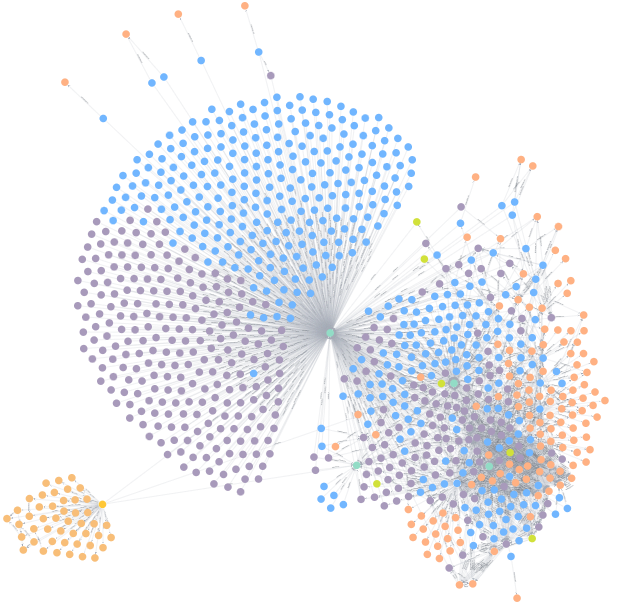
\includegraphics[width=\textwidth]{inc/figures/kg_full.png}
    \caption{Overview of the complete knowledge graph.}
    \label{fig:kg-full}
\end{figure}

The high \textsc{mentioned\_in} count (1,409, 40.4\%) reflects the provenance mechanism used to connect global entities to the guidelines in which they occur. These edges preserve cross-guideline occurrence information independently of more specific clinical relations. The next most frequent,
\textsc{recommended\_for}~(551), reflects the breadth of pharmacological
recommendations across the four families. The 438 \textsc{Drug} nodes and
462 \textsc{ClinicalCondition} nodes are high relative to the 5
\textsc{Condition} nodes. This reflects the schema design, in which a
small fixed set of canonical \textsc{Condition} nodes is pre-seeded,
while drug and clinical-condition mentions encountered during extraction may produce additional
nodes before synonym resolution.

\begin{figure}[!ht]
    \centering
    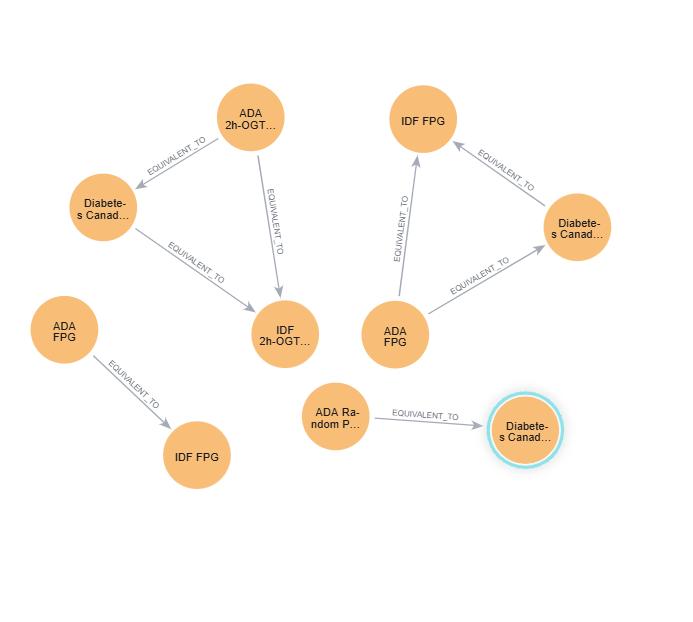
\includegraphics[width=\textwidth]{inc/figures/kg_equiv.png}
    \caption{Example of a cross-guideline equivalence relation in the knowledge graph.}
    \label{fig:kg-equiv}
\end{figure}

To illustrate the resulting graph structure at different levels of detail, Figure~\ref{fig:kg-equiv} shows an example of a cross-guideline equivalence relation. Figure~\ref{fig:kg-metformin} focuses on the neighbourhood of the drug metformin and illustrates how a single clinical entity can be connected to multiple relations and other entities. Finally, Figure~\ref{fig:kg-full} provides an overview of the complete knowledge graph.

\begin{figure}[!ht]
    \centering
    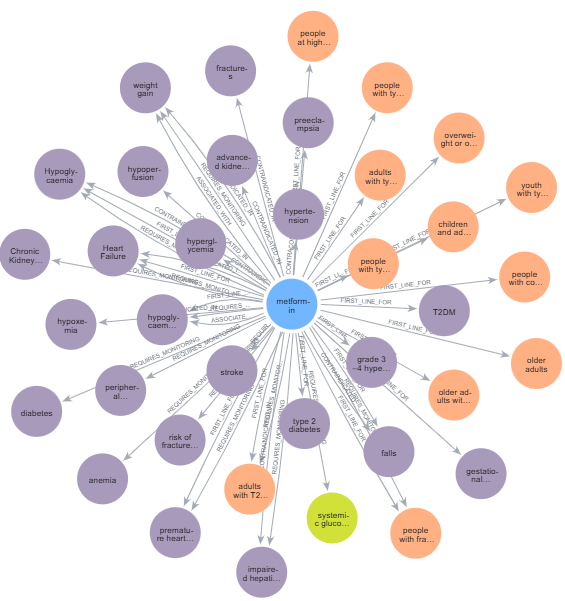
\includegraphics[width=\textwidth]{inc/figures/kg_metformin.png}
    \caption{Example of the graph neighbourhood of the drug metformin.}
    \label{fig:kg-metformin}
\end{figure}

\paragraph{Condition scoping of numerical targets.}
The extraction of a numerical target and its assignment to a diabetes
type are treated separately. A recognised numerical expression is maintained
as a \textsc{GlycaemicTarget} regardless of whether the surrounding text
identifies Type~1 or Type~2 diabetes. A disease-specific
\textsc{has\_target} relation is added only when the local context
identifies one of these types unambiguously.

This distinction was introduced after an implementation check showed that
the initial rule extractor used Type~2 Diabetes as the default condition
when no diabetes type could be determined from the local context. This
produced one \textsc{has\_target} relation for each of the 46 extracted
\textsc{GlycaemicTarget} nodes, even when the source text did not support
a Type~2-specific assignment. The condition-assignment rule was therefore
changed so that ambiguous targets remain in the graph without a
disease-specific relation.

With this correction, all 46 \textsc{GlycaemicTarget} nodes are retained,
while 24 \textsc{has\_target} relations are created. Seven originate from
the Type~1 Diabetes node and 17 from the Type~2 Diabetes node. Some targets
can be associated with both conditions when separate source contexts
support both assignments. The eight cross-guideline
\textsc{equivalent\_to} relations are unaffected because their construction
depends on the normalised target properties rather than on
\textsc{has\_target}.


\section{Question Generation}
\label{sec:exp_questions}

The question generation stage applies the three-function pipeline
$\gamma = \nu \circ \beta \circ \alpha$ defined in
Chapter~\ref{chap:construction} to the final Knowledge Graph,
where $\alpha$ is the graph-traversal targeting function,
$\beta$ is the language-model formulation function, and $\nu$ is
the rule-based validation function. In other words, a graph edge is
first selected as an anchor by $\alpha$, converted into question text
by $\beta$, and then checked against the same anchor by $\nu$.
This follows the schema-constrained prompting approach of
~\cite{caufield2024} and produces a validated catalogue
$\mathcal{Q}^+$.

Two question-generation runs are reported in this chapter and are analysed separately. The first run used Claude Opus 4.8 \footnote{Model identifier \texttt{claude-opus-4-8}, accessed through the Anthropic API, \url{https://docs.anthropic.com};}
 through the Anthropic API and was stopped before all eligible graph anchors had been processed because of practical token and cost constraints. This partial run produced a catalogue of 491 validated questions and was the source of the questions used in the human clinical review in Section~\ref{sec:exp_quality-human}. A subsequent run used gpt-4o-mini \footnote{Model identifier \texttt{gpt-4o-mini}, accessed through the OpenAI API, \url{https://platform.openai.com/docs/models}.}, using
the same final Knowledge Graph and provides the catalogue-level generation and validator statistics reported in this section. Results from the two runs are not pooled.

\subsection{Catalogue Overview}
\label{sec:q-overview}

In the GPT-4o-mini run, the targeting and generation pipeline produced 1,289 question records from eligible graph anchors. The rule-based validator accepted 1,280 questions (99.3\%) into \(\mathcal{Q}^+\) and routed 9 questions (0.7\%) to the flagged catalogue \(\mathcal{Q}^-\). No LLM fallback was required during this run. Of the 1,289 generated questions, 296 (23.0\%) were successfully produced with multiple-choice options, using LLM-generated distractors and a graph-locked correct answer. Of these, 294 were retained in the accepted catalogue after validation.


\subsection{Distribution by Relation Type}
\label{sec:q-by-relation}

Relation-type-driven question generation is an established approach in
knowledge-graph question generation. The distribution
reflects both the graph edge frequency and the per-type
sampling limits in $\alpha$.
Table~\ref{tab:q-relation} shows the question counts per relation type:
\textsc{recommended\_for} produces the most questions at 383, followed by
\textsc{manages} at 265, while \textsc{equivalent\_to}, despite drawing on only
eight graph edges, still produces 8 cross-guideline questions that no
single-guideline source could support.

\begin{table}[!ht]
\centering
\small\setlength{\tabcolsep}{8pt}
\begin{tabular}{p{4.2cm} r p{3.8cm}}
\hline
\textbf{Relation type} & \textbf{Questions} & \textbf{Question form} \\
\hline
\textsc{recommended\_for}    & 383 & \textit{which} \\
\textsc{manages}             & 265 & \textit{how} (vignette) \\
\textsc{mentioned\_in}       & 125 & \textit{which} (paraphrase) \\
\textsc{first\_line\_for}    & 117 & \textit{which} + MCQ \\
\textsc{associated\_with}    & 107 & \textit{what} \\
\textsc{contraindicated\_in} & 107 & \textit{yes/no} + MCQ \\
\textsc{second\_line\_for}   &  51 & \textit{which} + MCQ \\
\textsc{used\_with}          &  60 & \textit{what} \\
\textsc{requires\_monitoring}&  45 & \textit{what} \\
\textsc{has\_target}         &  21 & \textit{what} + MCQ \\
\textsc{equivalent\_to}      &   8 & \textit{how} \\
\hline
\textbf{Total}               & \textbf{1{,}289} & \\
\hline
\end{tabular}
\caption{Questions by relation type and question form.}
\label{tab:q-relation}
\end{table}


\begin{figure}[!ht]
    \centering
    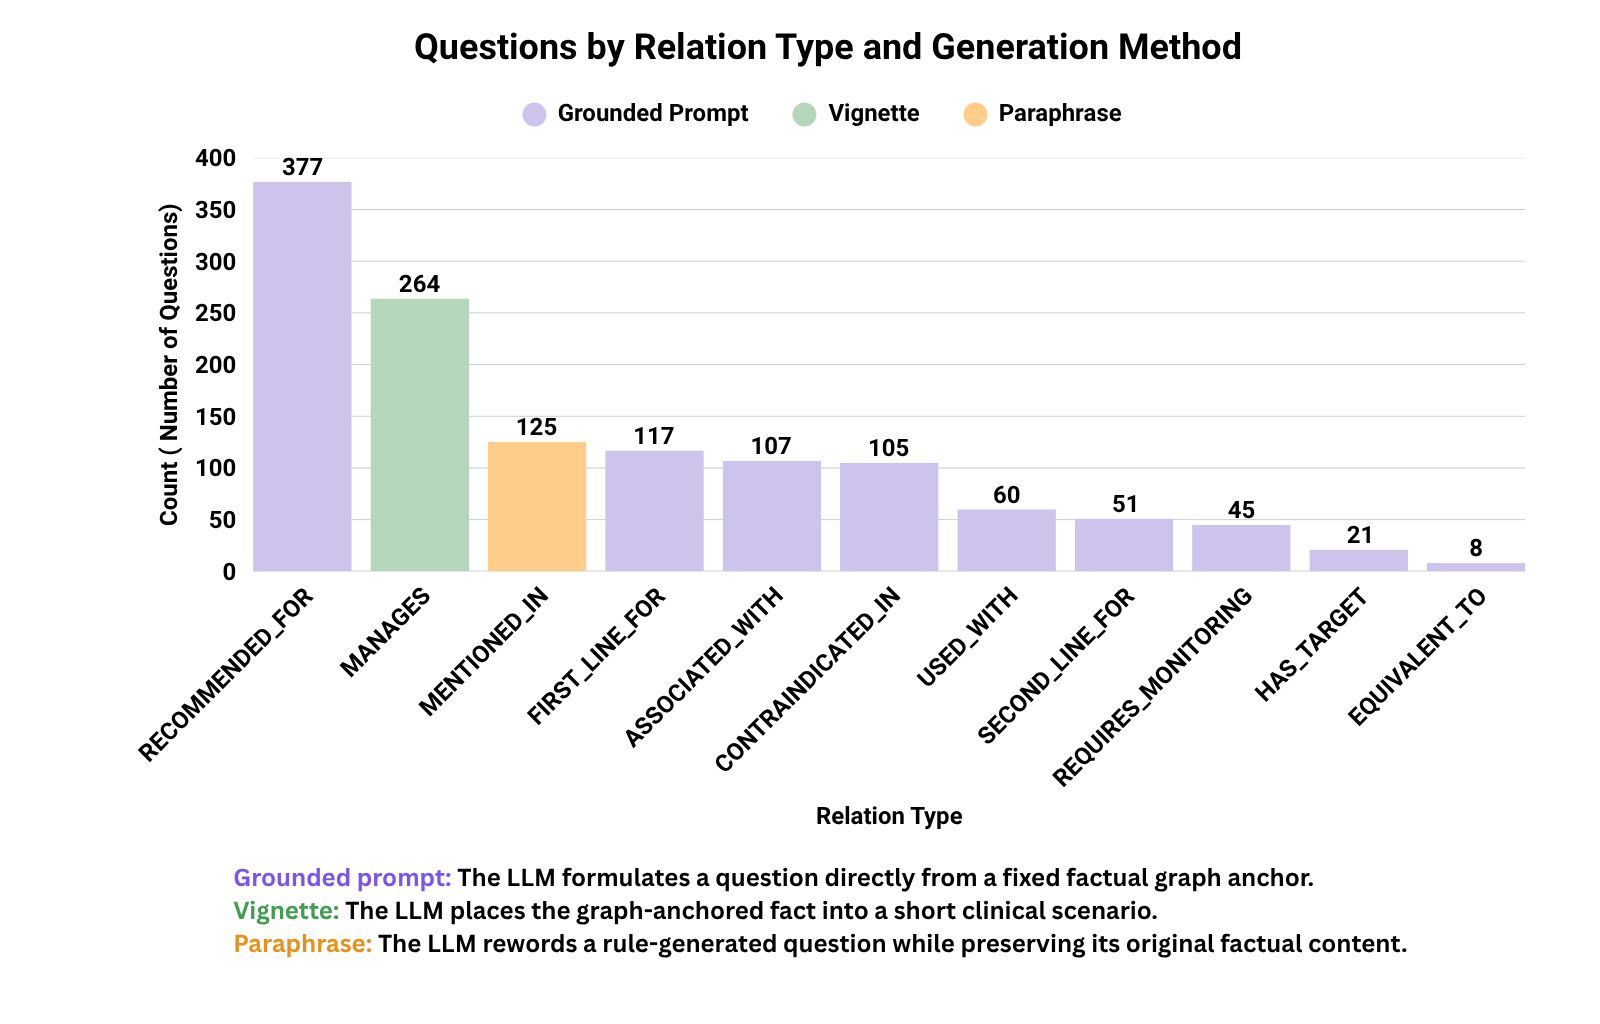
\includegraphics[width=\textwidth]{inc/figures/q_method.png}
    \caption{Question distribution by relation type and generation method.}
    \label{fig:q-method}
\end{figure}


Figure~\ref{fig:q-method} shows how the generated questions were distributed across the graph relation types and the three primary generation methods. The distribution reflects the fixed relation-to-method mapping used by the question-generation pipeline. Grounded prompts were used for relations where the answer could be directly formulated from the graph assertion, while clinical vignettes and template paraphrases were used for the corresponding relation types defined by the generation configuration.

\begin{figure}[!ht]
    \centering
    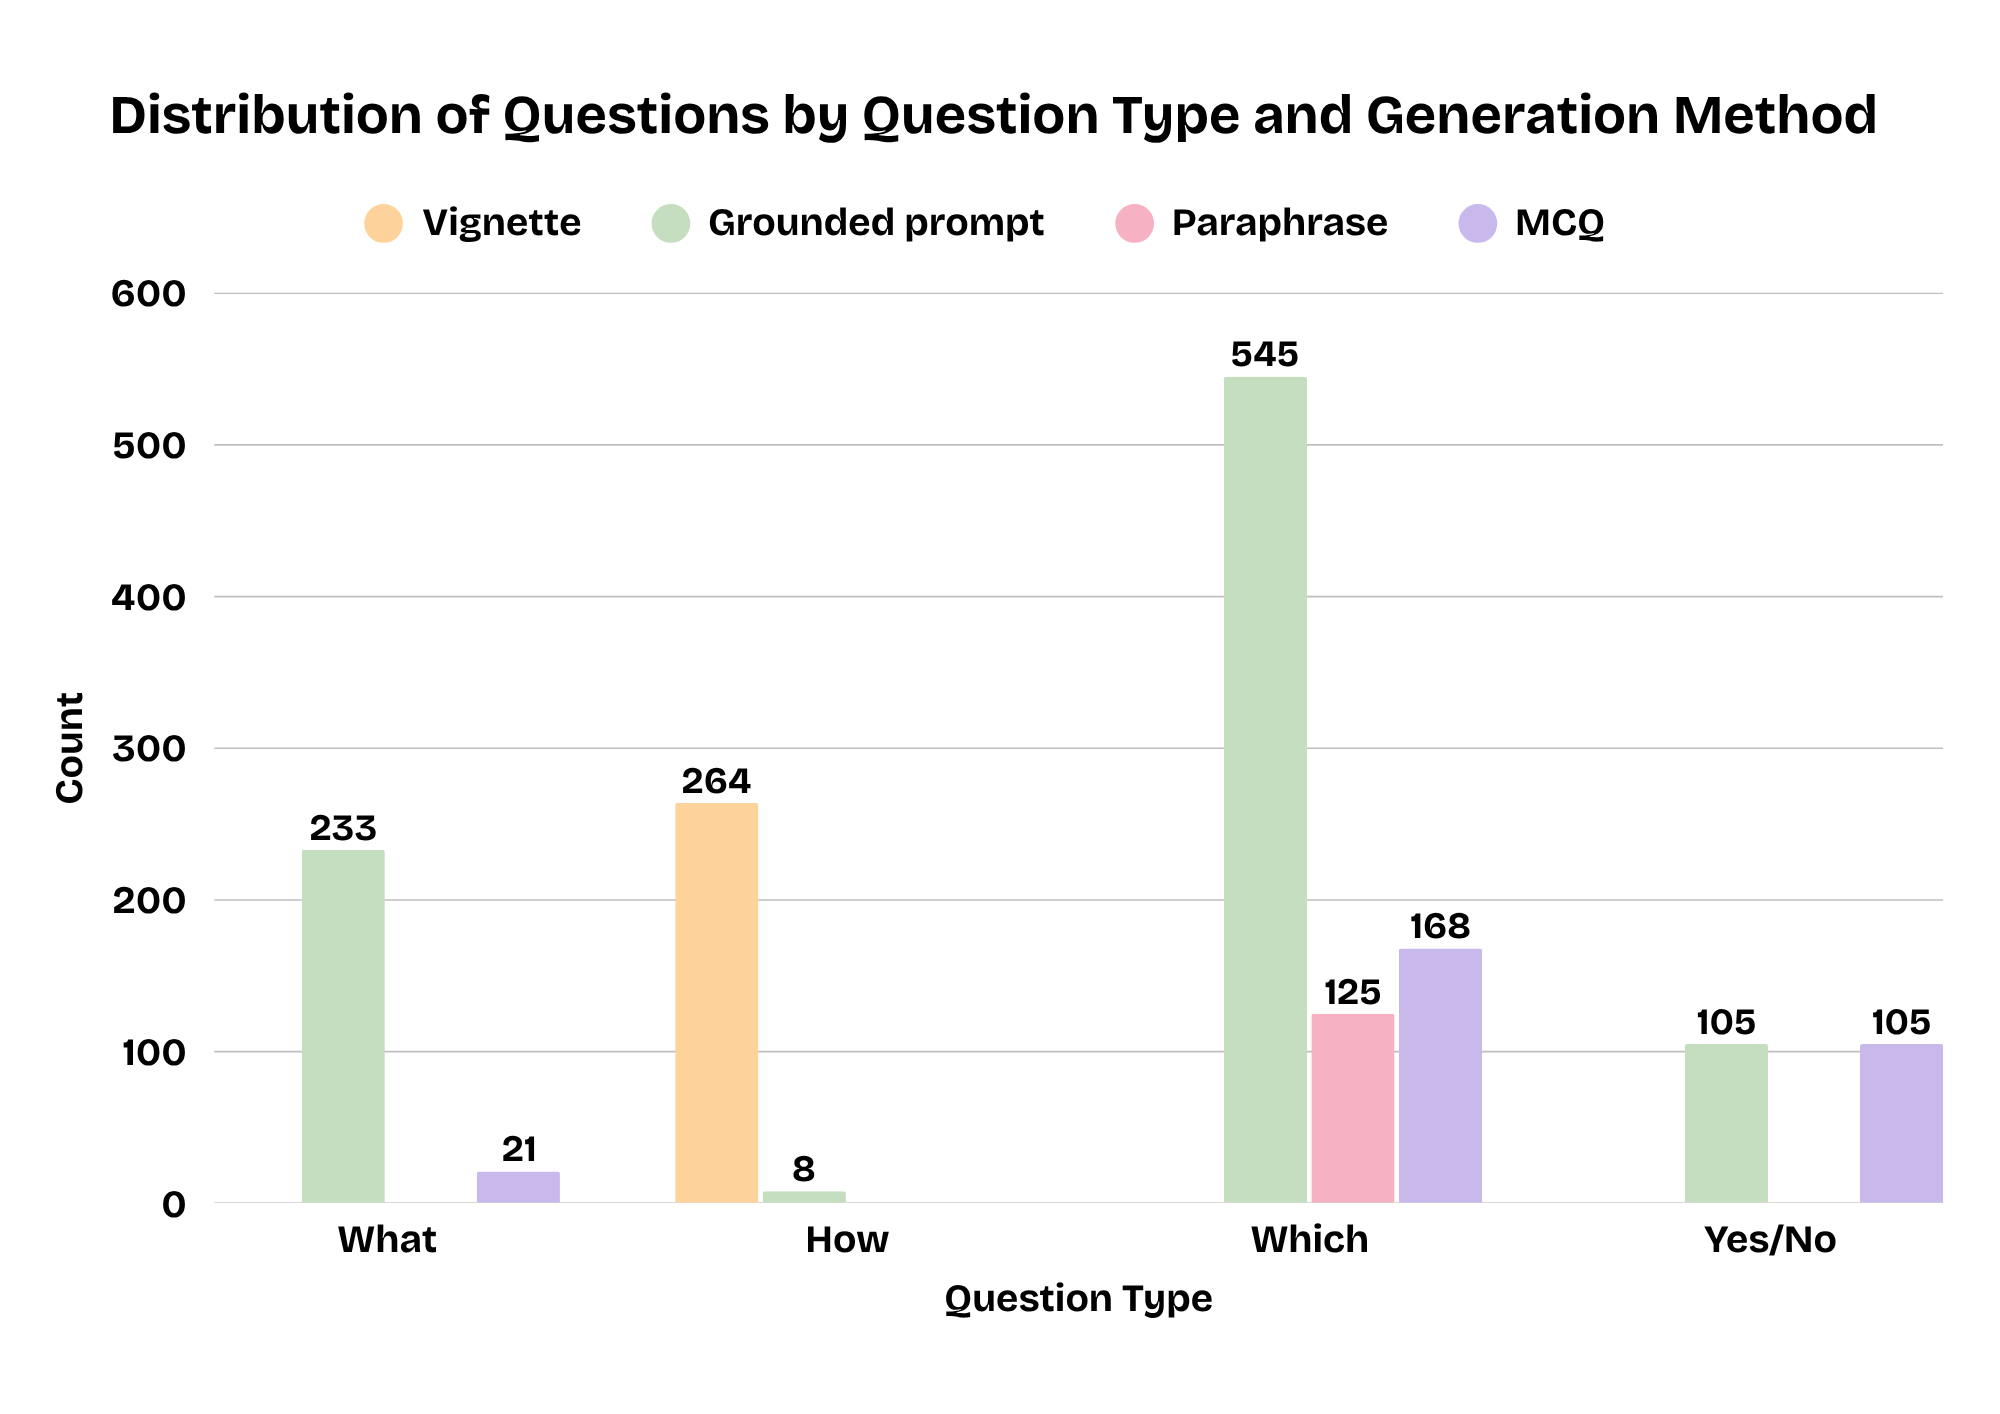
\includegraphics[width=\textwidth]{inc/figures/q_type.png}
    \caption{Distribution of accepted questions by question type, primary generation method, and MCQ format.}
    \label{fig:q-type}
\end{figure}

Figure~\ref{fig:q-type} shows the distribution of accepted questions across the four question types and the three primary generation methods. The figure also indicates which accepted questions were produced in multiple-choice format (MCQ). MCQ is treated as an output format rather than a separate generation method.

\subsection{Distribution by Generation Method and Question Type}
\label{sec:q-by-method}

\begin{table}[!ht]
\centering
\small
\begin{tabular}{lrr@{\hspace{1.5cm}}lrr}
\hline
\textbf{Method} & \textbf{N} & \textbf{\%} &
\textbf{Type} & \textbf{N} & \textbf{\%} \\
\hline
Graph-grounded prompt  & 899 & 69.7 & \textit{which}    & 676 & 52.4 \\
Clinical vignette      &    265  & 20.6 & \textit{how}  & 273 & 21.2 \\
Template paraphrase    &    125  & 9.7 & \textit{what}   & 233 & 18.1 \\
                       &         &      & \textit{yes/no} & 107 &  8.3 \\
\hline
\textbf{Total}         & 1{,}289 & 100  & \textbf{Total}  & 1{,}289 & 100 \\
\hline
\end{tabular}
\caption{Questions by generation method and question type in the full
         GPT-4o-mini catalogue.}
\label{tab:q-method}
\end{table}

The which form is the most frequent (52.4\%), driven primarily by \textsc{recommended\_for}, \textsc{first\_line\_for}, \textsc{second\_line\_for}, and the cross-guideline \textsc{mentioned\_in} questions. The how form accounts for 21.2\% and is dominated by the vignette-based \textsc{manages} relations. The yes/no form remains the least frequent (8.3\%) because it is restricted to \textsc{contraindicated\_in} edges.


\subsection{Cross-Guideline Questions}
\label{sec:cross-guideline-q}

The eight questions derived from \textsc{equivalent\_to} anchors are the only
ones in the catalogue requiring knowledge spanning two guidelines. Each anchor
pairs two \textsc{GlycaemicTarget} nodes from different organisations that
share the same normalised threshold. An example question from the
FPG $\geq 7.0$~mmol/L edge between ADA and Diabetes Canada:

\begin{quote}
\textit{What fasting plasma glucose threshold is shared by the ADA and
Diabetes Canada target nodes, and in what units does each guideline state
it?}
\end{quote}

This question type is not possible from a single-guideline pipeline in this corpus or by
extraction from raw text, because it depends on an \textsc{equivalent\_to}
edge that does not exist in any source document.

\subsection{Representative Examples}
\label{sec:q-examples}

Table~\ref{tab:q-examples} shows representative questions drawn from the
validated catalogue, grouped by generation method and question type. The
examples illustrate the linguistic variety the hybrid pipeline achieves
compared to a single fixed template: the grounded-prompt method produces
direct factual questions; the vignette method produces clinical scenario
questions that embed the same pharmacological fact in a patient narrative (the
patient details, such as age group, sex or symptoms, are added by the model
and are not drawn from the anchor);
and questions derived from \textsc{equivalent\_to} anchors require the
student to compare positions across two guidelines simultaneously.

\begin{table}[!ht]
\centering
\small\setlength{\tabcolsep}{6pt}
\begin{tabular}{p{2.4cm} p{2.8cm} p{8.0cm}}
\hline
\textbf{Method} & \textbf{Type} & \textbf{Question} \\
\hline
Graph-grounded prompt
  & \textit{which} (recall)
  & Which pharmacological approach is recommended for managing blood
    glucose in people with diabetes who are at higher risk of
    hypoglycaemia? \\[6pt]
Graph-grounded prompt
  & \textit{what} (recall)
  & What fasting plasma glucose level is used as the threshold for
    identifying individuals at risk of developing type~2 diabetes? \\[6pt]
Graph-grounded prompt + MCQ
  & \textit{what} (recall)
  & In a patient presenting with classic symptoms of hyperglycaemia,
    what random plasma glucose value meets the diagnostic threshold
    for diabetes mellitus?
    \newline
    \textit{A.}~$\geq 180.0$~mg/dL \quad
    \textit{B.}~$\geq 140.0$~mg/dL \quad
    \textit{C.}~$\geq 200.0$~mg/dL \quad
    \textit{D.}~$\geq 160.0$~mg/dL \\[6pt]
Clinical vignette
  & \textit{how} (application)
  & A middle-aged man with a history of type~2 diabetes and recently
    diagnosed stable heart failure presents for a routine medication
    review. He reports mild ankle swelling and reduced exercise
    tolerance. Which pharmacological management strategy should be
    prioritised given his dual diagnosis? \\[6pt]
Cross-guideline
  & \textit{how} (application)
  & How does the fasting plasma glucose threshold used to diagnose
    diabetes compare between the American Diabetes Association and
    Diabetes Canada guidelines? \\
\hline
\end{tabular}
\caption{Representative questions from the validated catalogue.}
\label{tab:q-examples}
\end{table}

\section{Evaluation of Question Quality}
\label{sec:exp_quality}

This section evaluates question quality beyond the automatic validator. A rule-based baseline is used to compare output variety, lexical diversity is assessed at catalogue level, and a sample from the partial Claude Opus 4.8 run is examined through independent clinical review.

\subsection{Baseline Definition}
\label{sec:exp_quality-baseline}

The baseline for comparison is a rule-only question generator that produces
one canonical question per anchor triple using a fixed directional template
per relation type. For a \textsc{recommended\_for} edge with source $v_s$ and
destination $v_d$, the canonical template produces: \textit{``Which drug is
recommended for $v_d$?''} with the answer fixed to $v_s$. No language model
is called, no reformulations are generated, and no MCQ distractors are
produced. Anchor consistency holds trivially here, because the question text
contains only the node names from the anchor. Hallucination in language
models is a well-documented problem~\cite{huang2025}; the validator is
designed specifically to catch faithfulness failures where the generated
text departs from the supplied anchor fact. The baseline represents the
minimum viable question catalogue: graph-anchored, consistently
structured, and producible without any LLM calls or additional cost.

The hybrid pipeline, described in Section~\ref{sec:exp_questions}, differs
from this baseline in three respects: the surface form of each question is
generated from an anchor-restricted prompt; reformulations
of the question are generated at up to three distinct phrasings; and
multiple-choice distractors are generated for selected relation types. The rule-only baseline is anchor-consistent by construction because its question and answer are assembled directly from the graph anchor. For the hybrid pipeline, anchor consistency is checked after language-model formulation by the rule-based validator, and only questions passing these checks enter the validated catalogue. Neither case implies that the underlying graph edge is clinically correct.

\subsection{Validator Analysis}
\label{sec:validator-analysis}

The validator applies three checks to every generated question. Check~1
verifies that the correct answer appears in the question text or is
recoverable as a named graph entity. Check~2 flags any number in the
generated question that was not present in the anchor's node properties
(with small integers 0--4 whitelisted as non-clinical). Check~3 verifies
that if a specific guideline is named in the question, it matches the anchor's
issuing organisation.

Nine questions were routed to \(\mathcal{Q}^-\), all because Check~2 detected numerical information in the generated question that was not represented among the numerical properties permitted by the validator. Six originated from \textsc{recommended\_for} relations, two from \textsc{contraindicated\_in}, and one from a \textsc{manages} relation. The flagged values included patient ages or age ranges, a postpartum duration, an eGFR range, and an age introduced in a vignette. Inspection showed that several of these values reflected information embedded in population or condition descriptions rather than newly invented clinical thresholds. The numerical validator is therefore deliberately conservative and can flag contextually appropriate numbers when they are not represented in the specific anchor properties it checks. The resulting 99.3\% acceptance rate measures consistency with the implemented validation rules rather than clinical accuracy.


\subsection{Automatic Metrics}
\label{sec:exp_quality-automatic}

Table~\ref{tab:quality-auto} compares the hybrid pipeline against the rule-only
baseline: the hybrid pipeline generates 294 multiple-choice questions and 3.38
phrasings per anchor on average, against none and exactly 1.00 for the rule-only
baseline. The validator pass rate is lower for the hybrid pipeline (99.3\%
against 100\%) for the reasons discussed in Section~\ref{sec:validator-analysis}.

\begin{table}[!ht]
\centering
\small\setlength{\tabcolsep}{8pt}
\begin{tabular}{lcc}
\hline
\textbf{Metric} & \textbf{Rule-only baseline} & \textbf{Hybrid pipeline} \\
\hline
Validator pass rate     & 100\%   & 99.3\% \\
Questions with MCQ      & 0       & 294 \\
Mean phrasings/anchor   & 1.00    & 3.38 \\
MSTTR (window 50)       & n/a     & 0.716 \\
Primary difficulty labels       & n/a       & 2 (recall, application)\\
\hline
\end{tabular}
\caption{Automatic metrics for the rule-only and hybrid pipelines.}
\label{tab:quality-auto}
\end{table}

The main quantitative difference between the two approaches is the variety of question forms produced.
The accepted GPT-4o-mini catalogue contains 1,280 primary questions and 3,048 stored reformulations, giving 4,328 phrasings in total. To describe this variation, the mean number of stored phrasings per accepted anchor is calculated as

\[
\text{Mean phrasings per anchor}
=
\frac{N_{\mathrm{primary}} + N_{\mathrm{reformulations}}}
     {N_{\mathrm{primary}}}.
\]

Since each primary question corresponds to one accepted graph anchor, this gives
\[
\frac{1280 + 3048}{1280} = 3.38
\]
stored phrasings per anchor.

Lexical diversity is measured using the Mean Segmental Type--Token Ratio (MSTTR)~\cite{Ahn2025}. Unlike the conventional type--token ratio, MSTTR reduces the effect of text length by calculating lexical diversity over equal-length, non-overlapping segments:

\[
\mathrm{MSTTR}
=
\frac{1}{k}\sum_{i=1}^{k}\frac{t_i}{w_i},
\]

where \(k\) is the number of segments, \(t_i\) is the number of unique word types in segment \(i\), and \(w_i\) is the number of tokens in that segment. Using a 50-token window across the primary questions and their reformulations gives an MSTTR of 0.716.

The accepted catalogue also contains 294 questions with MCQ options. Primary questions are labelled as either recall or application depending on the generation method, while the reformulations additionally include analysis variants. In comparison, the rule-only baseline produces a single phrasing per anchor, does not generate MCQ options, and does not assign difficulty labels.

\subsection{Human Clinical Review}
\label{sec:exp_quality-human}

A sample of 30 questions from the 491-question partial Claude Opus 4.8 catalogue was reviewed for clinical soundness by two medical doctors. The questions were presented without the graph anchors that produced
them, so that each reviewer judged the question on its own clinical merits
rather than against the system's intended answer. The two review sets of 15
questions each were non-overlapping and sampled across generation methods in
proportion to their frequency in the catalogue.

Evaluation of clinical NLP systems often relies on comparison against
expert-annotated reference standards \cite{uzuner2011}, and for
generated clinical text, evaluation by physicians has been used to assess
quality along clinical dimensions \cite{singhal2025}.
Each reviewer was asked to mark each question as clinically correct or
incorrect, and to provide one line of explanation for any question marked
incorrect. Both reviewers are qualified medical doctors from India and were contacted through the author's personal network. Dr. Mounika is currently in the final year of postgraduate training in Obstetrics and Gynaecology. Dr. Aakanksha completed her undergraduate medical education in India, and is currently preparing for the Fachsprachprüfung (FSP) in Heidelberg, Germany as part of the process of continuing medical practice in Germany. Both participated voluntarily and without compensation, and agreed to take part and to be described in this thesis. The review involved no patients and no personal data beyond the reviewers' professional background reported here. Each reviewed a separate set of 15 questions, so the
two sets do not overlap and no question was seen by both reviewers. Reviewers
worked independently and were not in contact with each other during the
review. They were shown the question text only, without the graph anchor, the
answer key, or the source guideline passage, so each judgement was made on the
question as a learner would encounter it. The reviewers were also not informed which language model had generated the questions. Because the guidelines in the corpus are American, British, Canadian, and international, reviewers were asked to indicate where a flag reflected a difference from routine practice in their own clinical context rather than a factual error in the question.

The human review showed that most questions were considered acceptable, while several issues were identified in the reviewed sample. Table~\ref{tab:quality-human} summarises the individual review results, while Figure~\ref{fig:review} shows the distribution of the review outcomes for the two reviewers. The following discussion examines the identified issues in more detail.

\begin{table}[!ht]
\centering
\small\setlength{\tabcolsep}{5pt}
\begin{tabular}{p{0.5cm} p{1.8cm} p{5.0cm} p{4.8cm}}
\hline
\textbf{Q} & \textbf{Reviewer} & \textbf{Reviewer comment} & \textbf{Root cause} \\
\hline
Q9
  & Dr. Aakanksha
  & Metformin identified as managing hypoglycaemic events; sulfonylureas
    are the drug class associated with hypoglycaemia
  & Extraction error: the source passage does not support the extracted \texttt{metformin --MANAGES--> hypoglycaemic events} relation \\[4pt]

Q15
  & Dr. Aakanksha
  & NHS Path to Remission recommended for Heart Failure; SGLT2 inhibitors
    are the standard pharmacological approach for T2DM with Heart Failure
    & Extraction error: the source passage does not support the extracted
    \texttt{manages} relation between this programme and Heart Failure \\[4pt]
Q3
  & Dr. Mounika
  & No specific antidiabetic is recommended for fractures; perioperative
    glycaemic control is managed by insulin dose adjustment only
  & Extraction error: the source passage does not support the extracted \texttt{insulin --RECOMMENDED\_FOR--> fractures} relation \\[4pt]
Q6
  & Dr. Mounika
  & Bariatric surgery for T2DM is evidence-based but not routine practice;
    noted as practised differently in India
  & Clinical scope: ADA and IDF guidelines do recommend metabolic surgery
    for eligible adults with T2DM; not an extraction error \\
\hline
\end{tabular}
\caption{Human clinical review results.}
\label{tab:quality-human}
\end{table}

\begin{figure}[!ht]
    \centering
    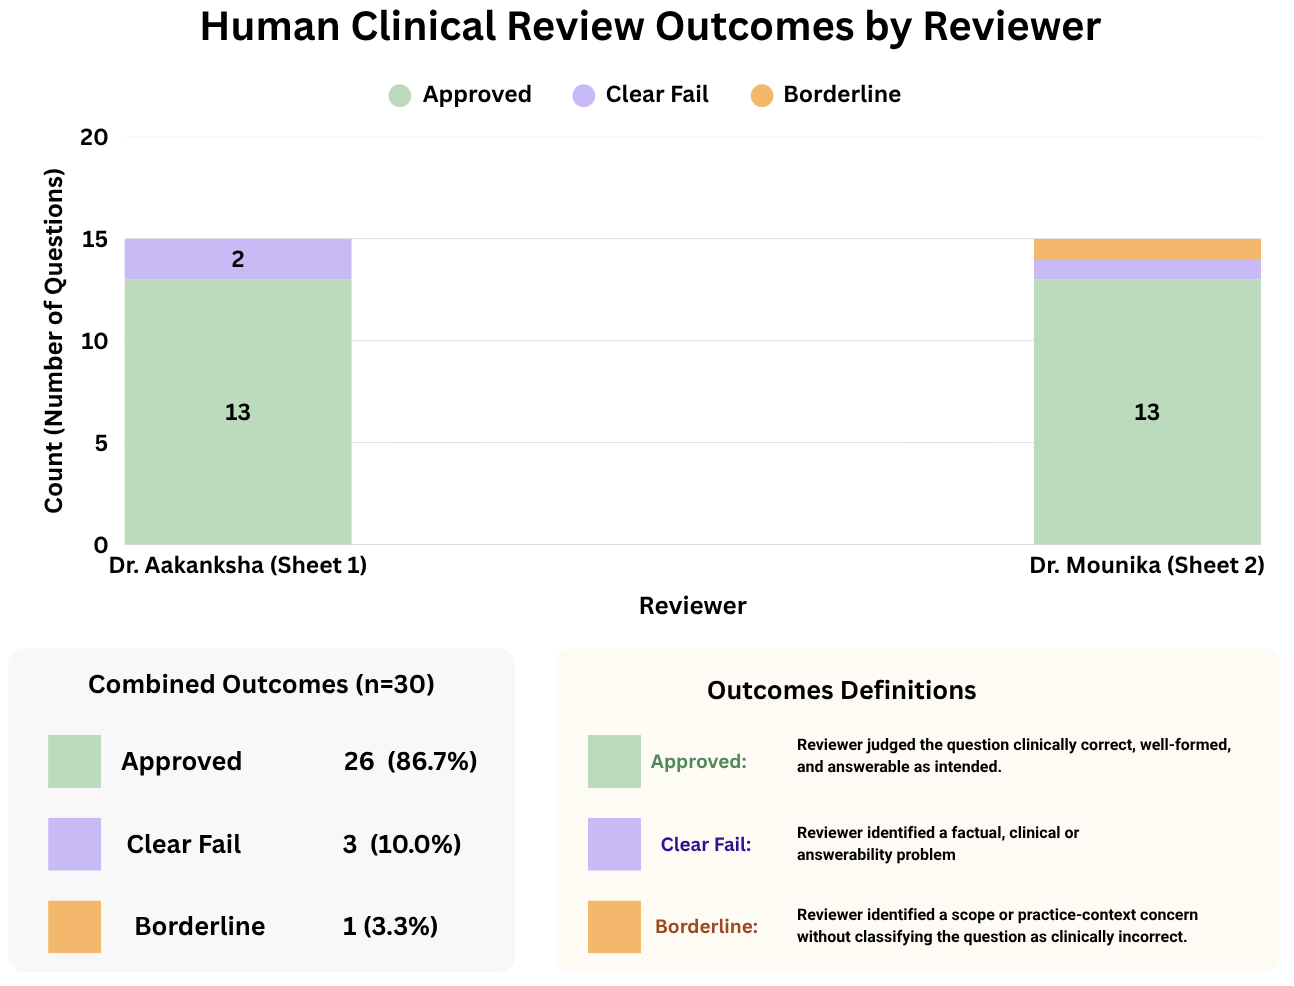
\includegraphics[width=0.75\textwidth]{inc/figures/review.png}
    \caption{Human clinical review outcomes by reviewer.}
    \label{fig:review}
\end{figure}


Of the 30 reviewed questions, 26 were accepted without qualification.
Three were classified as clear failures and were traced to incorrect
relations in the Knowledge Graph. One additional question (Q6) was
flagged because its content, although supported by the source guidelines,
was outside routine practice in the reviewer's clinical context. This
case is therefore treated as a clinical-scope flag rather than a factual
error.

Within this sample, all three clear failures originated from incorrect
graph relations rather than from the question-formulation step. The
sample is too small to establish a general reliability rate, but it
indicates that graph quality was the main source of factual error among
the reviewed questions.

One additional question was flagged by Dr. Aakanksha (Q5), which asked how the ADA
and IDF diagnostic thresholds for the 2-hour oral glucose tolerance test
compare. The reviewer noted that both guidelines use the same
threshold of $\geq 11.1$~mmol/L, which is the intended answer to the
question. This confirms that the cross-guideline comparison question type
produced from \textsc{equivalent\_to} edges is answerable. It is not counted as a failure.



\subsection{Comparison with Baseline}
\label{sec:exp_quality-comparison}

Clinical correctness against the original guideline sources was not independently measured for the rule-only baseline, so the comparison is limited to properties of the generated catalogue rather than clinical accuracy.The accepted hybrid catalogue contains 1,280 primary questions together with 3,048 additional reformulations and 294 questions with MCQ options. Primary questions carry recall or application difficulty labels, while the stored reformulations additionally include recall, application, and analysis variants. This provides a wider range of question forms than the fixed single-phrasing rule-only baseline. Whether this additional variety translates into improved learning outcomes is not evaluated in this thesis and remains a question for future study.



\section{Limitations}
\label{sec:exp_limitations}

The experiments and the final implementation showed several limitations
that would need to be addressed in further work.

\paragraph{Entity matching.}
Drug and clinical-condition names are merged using fixed alias lists.
This works for the variants included in those lists, but an alternative
name that is not listed can remain as a separate node. The current
implementation therefore depends on knowing common naming variations in
advance. Extending the alias lists would improve coverage, although the
additional mappings would need to be checked to avoid merging different
clinical concepts.

\paragraph{Cross-guideline target comparison.}
The current \textsc{equivalent\_to} comparison is limited to
plasma-glucose targets that have a value in mmol/L. HbA1c targets are
also extracted, and conversions between percentage and mmol/mol are
stored, but these values are not included in the equivalence comparison.
The eight equivalence relations reported in this chapter therefore cover
only the plasma-glucose targets matched by the implemented criterion.

\paragraph{Condition scoping.}
The diabetes type of a numerical target is determined from the text in
which the target is extracted. If that text mentions both Type~1 and
Type~2 diabetes, or does not identify either one, the target is kept but
no disease-specific \textsc{has\_target} relation is added. This is safer
than assigning a default condition, but some targets consequently remain
without a Type~1 or Type~2 link. Section or document context could be used
in addition to the local text in a future version.

\paragraph{Contextual extraction.}

Contextual entity and relation extraction contributes directly to the final Knowledge Graph used by both question-generation runs. Although the LLM extractor is constrained through the prompt to predefined entity and relation types and is instructed not to introduce relations unsupported by the source passage, these constraints are not enforced independently against the original guideline after extraction. Errors introduced during contextual extraction can propagate into the final graph and subsequently into generated questions. This was observed during human review, where some clinically questionable questions remained consistent with incorrect or questionable graph relations. Since the question validator checks graph-anchor consistency rather than independently verifying the source guideline, such upstream errors are outside its scope. A systematic source-level evaluation of contextual extraction was not carried out and remains future work.

\paragraph{Generalisability.}
The pipeline was evaluated only on the diabetes guideline corpus used in
this thesis. Several ingestion rules are specific to the four publishing
formats in the corpus. For example, the implementation contains separate
handling for ADA recommendation blocks, NICE document structure, IDF
care-level recommendations, and Diabetes Canada text extraction. A new
guideline family may therefore require additional document-specific
handling before the rest of the pipeline can be applied.

\chapter{Conclusions and Future Work}
\label{chap:conclusion}

\section{Conclusion and Key Findings}
This thesis addressed a practical problem: clinical practice guidelines
from different organisations are distributed across heterogeneous documents
and are not directly available in a common representation for
cross-guideline querying and comparison. The approach taken was to construct
a knowledge graph that represents content from multiple guidelines in a
shared structure and then use that graph as a controlled source for
question generation.

The four-stage pipeline: ingestion, extraction, normalisation, and question
generation, was designed to handle the structural and terminological
variation that arises when documents from different publishing
organisations are processed together. The ingestion stage classified
document content into typed element records while preserving page-level
provenance. The extraction architecture separates entity types between a
rule-based layer and a contextual layer, with the full design supporting
LLM-based extraction for categories that require contextual interpretation.
The normalisation stage resolved duplicate entities, converted measurement
units to a common representation, and created equivalence edges between
matching targets from different organisations. The question-generation
stage selected graph edges as anchors, provided each anchor to the language
model as factual context, and checked the generated question for consistency
with that anchor before acceptance.

The pipeline was instantiated on eight documents from four organisations
covering Type~1 and Type~2 diabetes. The resulting knowledge graph contains
2,503 nodes across 13 node types and 3,485 edges across 18 relation types.
Normalisation created eight \textsc{equivalent\_to} edges linking matching
diagnostic thresholds across ADA, IDF, and Diabetes Canada after unit
conversion. These relations are not directly stated in any individual
source document; they arise from comparing independently stated targets
after normalisation.

The full GPT-4o-mini question-generation run produced 1,289 questions, of which 1,280 passed the rule-based validation checks and 9 were flagged by the rule-based validator because they contained numerical values absent from their anchors. A separate 491-question
catalogue was used for the detailed quality evaluation. From this catalogue, 30 questions were reviewed by two medical doctors:
26 were accepted without qualification, three contained clear
extraction-derived errors, and one was flagged for a clinical-scope
concern rather than a factual error.

In the reviewed sample, all three clear failures were traced to incorrect
graph relations rather than to the question-formulation step. This points to graph quality, particularly the correctness of extracted relations, as an important target for further improvement.

\section{Future Work}

Several directions follow from the work reported here.

The ingestion pipeline evaluated Docling as an alternative to PyMuPDF but did
not adopt it, primarily because of its runtime cost on the CPU-only development
hardware (Section~\ref{sec:exp_parsing}). A spot check on a small sample showed
Docling produced no ligature artefacts, unlike the PyMuPDF output, though the
comparison of word-spacing errors between the two was inconclusive. With GPU
acceleration available, re-evaluating Docling as the primary parser,
particularly for its ligature handling, would be a reasonable next step, and
could reduce or replace the family-specific text repairs currently required for
some document sources.

The LLM-based contextual extraction path was executed for the four entity categories of drugs, clinical conditions, populations, and interventions. However, extraction quality was not independently evaluated against a manually annotated gold-standard dataset, and the LLM-based extraction was not compared with the heuristic fallback mode of the same script.

Entity deduplication in this work is deterministic and relies on a fixed
synonym dictionary. Surface forms not represented in the dictionary remain
as separate nodes, which can increase the number of near-duplicate Drug and
ClinicalCondition nodes. Embedding-based or fuzzy matching could improve
recall in entity resolution, although safeguards would be needed to avoid
incorrectly merging distinct entities.

The current \textsc{equivalent\_to} criterion is implemented for normalised
plasma-glucose targets. Although alternate HbA1c representations are stored
during extraction, the equivalence procedure does not currently compare
HbA1c targets across organisations. Extending the criterion to HbA1c would
enable additional cross-guideline comparisons, including comparisons
involving NICE targets represented in the corpus.

The validator checks consistency between a generated question and its graph
anchor, but it does not determine whether the underlying graph relation is
clinically correct. A more complete evaluation would include a larger
reviewed sample, reviewers with a broader range of relevant clinical
expertise, and an analysis of whether the graph errors observed in the
current review are systematic or isolated.

Finally, the four-stage architecture is not tied to diabetes, but the
schema, extraction rules, canonical entities, repair procedures, and
normalisation configuration used here were developed for the diabetes
corpus. Applying the architecture to another multi-guideline domain would
test which components transfer with limited adaptation and which require
domain-specific redesign.

% Bibliography
\newpage

\bibliographystyle{apalike}
\bibliography{references}
\nocite{*}

\appendix
\chapter{Prompts and Human Review Material}
\section{LLM Extraction Prompts}
\label{app:extraction-prompts}

The following prompts were used in
\texttt{llm\_extract\_relations.py} for schema-constrained
entity and relation extraction. The system prompt defines the
output schema and extraction rules. The user prompt supplies
the guideline identifier, page number, known entities on the
page, and the raw text chunk to process.

\subsection*{System Prompt}

\begin{lstlisting}[language={},
  basicstyle=\small\ttfamily,
  breaklines=true,
  frame=single,
  caption={LLM extraction system prompt.}]

You are a clinical knowledge graph extractor specialising in diabetes guidelines.

Extract ONLY the following entity types from the TEXT:
{entity_type_descriptions}

Extract ONLY the following relation types:
{relation_type_descriptions}

RULES:
- Return STRICT JSON with keys: "entities" (list) and "relations" (list).
- Each entity needs: "id" (short unique string within this response), "type" (from the list above), "name" (canonical name), "organization" (which guideline this came from).
- Each relation needs: "type" (from list above), "from" (entity id), "to" (entity id).
- Drug names: use the most specific name mentioned. If a class is mentioned (e.g. SGLT2 inhibitor), create a class entity. If a specific drug is mentioned (e.g. empagliflozin), create both.
- Do NOT extract GlycaemicTarget, Recommendation, or numeric thresholds -- those are handled separately.
- Do NOT invent relations not explicitly stated in the text.
- If nothing relevant is found, return: {{"entities": [], "relations": []}}
- Return ONLY JSON. No markdown fences. No commentary.

\end{lstlisting}
\subsection*{User Prompt Template}
\begin{lstlisting}[language={},
  basicstyle=\small\ttfamily,
  breaklines=true,
  frame=single,
  caption={LLM extraction user prompt template. Placeholders in
           braces are substituted at runtime.}]
GUIDELINE: {org} ({year})
PAGE: {page}

KNOWN FACTS ON THIS PAGE (already extracted -- do not re-extract these):
{known_facts}

TEXT:
{chunk_text}

Return ONLY JSON.
\end{lstlisting}
\newpage
\section{Question Generation Prompts}
\label{app:qgen-prompts}

The following system and user prompts were used in
\texttt{generate\_questions\_hybrid.py}.
Each generation method has a dedicated builder function that
constructs both prompts from the graph anchor at runtime.
Placeholders in braces are substituted from the anchor fields.


\subsection*{Graph-Grounded Prompt}

\begin{lstlisting}[language={},
  basicstyle=\small\ttfamily,
  breaklines=true,
  frame=single,
  caption={System prompt: Graph-Grounded Prompt.}]
You are a clinical medical education assistant.  You write clear, accurate questions for healthcare students studying diabetes management.  Use only the clinical information in the FACT block; do not add drug names,  thresholds, or guidelines that are not stated there.  Write the question as a standalone exam question.  Never refer to 'the fact', 'the provided fact', 'the context', 'the passage',  or the guideline source inside the question. A student reading the question  must not be able to tell it was generated from a supplied fact.
\end{lstlisting}

\begin{lstlisting}[language={},
  basicstyle=\small\ttfamily,
  breaklines=true,
  frame=single,
  caption={User prompt template: Graph-Grounded Prompt.}]
{context}

Task: Write ONE clinical {qtype} question that tests knowledge of this fact.
{focus_line}- The question must be answerable from the FACT above
- Do not mention page numbers, guideline names, or 'the provided fact'
- Write in clear, professional clinical language
- Output ONLY the question text, nothing else
\end{lstlisting}
\newpage
\subsection*{Clinical Vignette}

\begin{lstlisting}[language={},
  basicstyle=\small\ttfamily,
  breaklines=true,
  frame=single,
  caption={System prompt: Clinical Vignette.}]
You are a clinical medical education assistant writing case-based questions  for diabetes management training.  IMPORTANT: Base the clinical scenario ONLY on the facts provided.  You may describe the patient's condition and symptoms in words,  but must NOT include any numerical values (no ages, no HbA1c values,  no glucose readings, no doses) and must NOT introduce drug names,  targets, or guidelines beyond what is stated in the CLINICAL FACT block.
\end{lstlisting}


\begin{lstlisting}[language={},
  basicstyle=\small\ttfamily,
  breaklines=true,
  frame=single,
  caption={User prompt template: Clinical Vignette.}]
{context}

Task: Write a short clinical vignette question (2-3 sentences).
- Describe a realistic patient with {dst_name} using only words (no numbers)
- End with a question about pharmacological management
- The correct answer must be {src_name} (but do not give it away in the question)
- Do NOT include any numerical values in the question
- Output ONLY the question text, nothing else
\end{lstlisting}

\subsection*{Question Reformulation}

\begin{lstlisting}[language={},
  basicstyle=\small\ttfamily,
  breaklines=true,
  frame=single,
  caption={System prompt: Question Reformulation.}]
You are a clinical medical education assistant.  You rephrase questions for different difficulty levels without changing the factual content.
\end{lstlisting}

\begin{lstlisting}[language={},
  basicstyle=\small\ttfamily,
  breaklines=true,
  frame=single,
  caption={User prompt template: Question Reformulation.}]
Original question: "{canonical}"

Task: Rewrite this question at three difficulty levels.
Return ONLY a JSON object with this exact structure:
{{
  "recall":      "direct factual question (easiest)",
  "application": "clinical scenario requiring application of the fact",
  "analysis":    "comparative or reasoning question (hardest)"
}}
Do not change any drug names, numerical values, guideline names, or clinical facts.
\end{lstlisting}

\subsection*{MCQ Distractor Generation}

\begin{lstlisting}[language={},
  basicstyle=\small\ttfamily,
  breaklines=true,
  frame=single,
  caption={System prompt: MCQ Distractor Generation.}]
You are a clinical medical education expert creating multiple-choice questions  for diabetes pharmacology assessment.
\end{lstlisting}

\begin{lstlisting}[language={},
  basicstyle=\small\ttfamily,
  breaklines=true,
  frame=single,
  caption={User prompt template: MCQ Distractor Generation.}]
Question: {question}
Correct answer: {correct_answer}

Task: Generate exactly 3 wrong but plausible distractor options for this multiple-choice question.
Rules:
- Distractors must be real diabetes medications or clinical values (choose from: {pool_str})
- Do NOT include "{correct_answer}" as a distractor
- Distractors should be clinically plausible (a student could reasonably consider them)
- Return ONLY a JSON object with this exact structure: {{"distractors": ["option1", "option2", "option3"]}}
\end{lstlisting}

\newpage
\section{Human Review Question Set 1 (Reviewer: Dr.~Aakanksha)}
\label{app:review-set-1}

Reviewers were shown the question text only, without the graph anchor,
answer key, or source guideline passage.

\begin{enumerate}
\item A middle-aged woman with a longstanding history of type 2 diabetes presents to her nephrologist with progressive decline in kidney function, persistent proteinuria, and signs of fluid retention consistent with chronic kidney disease. She has been struggling to achieve adequate glycemic control despite lifestyle modifications, and her physician is considering adding a pharmacological agent specifically indicated for managing chronic kidney disease in patients with her underlying condition. Which patient population is the primary target for this kidney-protective pharmacological management strategy?

\item In a patient undergoing an oral glucose tolerance test, what 2-hour plasma glucose value meets the diagnostic threshold for type 2 diabetes?

\item In the management of type 2 diabetes mellitus, which pharmacological approach involving the combination of agents within a single preparation is recommended as a treatment strategy?

\item In a patient with type 2 diabetes, at what HbA1c threshold would a value be considered above the acceptable glycemic target, indicating suboptimal long-term blood glucose control?

\item How does the 2-hour plasma glucose threshold used to diagnose diabetes on an oral glucose tolerance test according to the American Diabetes Association compare with the threshold recommended by the International Diabetes Federation?

\item In a patient with type 2 diabetes, what is the target fasting plasma glucose level that indicates optimal glycemic control?

\item Which non-pharmacological intervention is recommended as part of the management plan for a patient diagnosed with diabetes?

\item Which medication, a glucagon-like peptide-1 receptor agonist, is recommended for the management of type 2 diabetes mellitus?

\item A middle-aged woman with a longstanding history of type 2 diabetes presents to her general practitioner reporting recurrent episodes of shakiness, sweating, and light-headedness occurring throughout the week, consistent with hypoglycaemic events. She has no known drug allergies and is currently not on any glucose-lowering therapy. Which oral pharmacological agent is indicated to manage her hypoglycaemic events?

\item In the management of diabetes, which medication is recommended for individuals who are unable to tolerate other pharmacological treatments?

\item A middle-aged man with longstanding type 2 diabetes attends a review clinic at a busy urban practice serving a socioeconomically disadvantaged community. He reports difficulty affording medications, has limited access to healthy food, and faces significant barriers to engaging with lifestyle programmes. Which patient population characteristic is particularly relevant when considering the pharmacological management approach for his type 2 diabetes?

\item Which class of medication is recommended for use in adults with type 2 diabetes: SGLT2 inhibitors?

\item Which pharmacological agent is recommended for the management of diabetes in elderly male patients?

\item A middle-aged woman with type 2 diabetes presents to her endocrinologist for a routine follow-up. She has a prior history of ischemic stroke and her physician is considering an oral antidiabetic agent that may offer additional benefit given her cerebrovascular history. Which pharmacological agent would be most appropriate to initiate in this patient to address both her glycemic management and her history of stroke?

\item Which structured programme is recommended for individuals with type 2 diabetes who also have Heart Failure, with the aim of achieving disease remission?

\end{enumerate}

\section{Human Review Question Set 2 (Reviewer: Dr.~Mounika)}
\label{app:review-set-2}

Reviewers were shown the question text only, without the graph anchor,
answer key, or source guideline passage.

\begin{enumerate}
\item A patient with type 1 diabetes mellitus is found to have impaired hypoglycaemic awareness. Based on established clinical recommendations, which intervention is advised for managing this condition?

\item A middle-aged man with type 1 diabetes attends a follow-up appointment reporting persistent postprandial hyperglycemia, particularly after his evening meals, which typically consist of large portions of grilled meat, cheese, and nuts. He describes these meals as very filling and rich, with minimal carbohydrate content but substantial amounts of fat and protein. What pharmacological agent is most appropriate to manage his glycemic response to these high-fat, high-protein mixed meals?

\item A patient with diabetes who sustains a fracture requires adjustment to their antidiabetic regimen. Which antidiabetic agent is recommended for use in the setting of a fracture?

\item Which oral antidiabetic agent is recommended as a pharmacological treatment for children and adolescents diagnosed with type 2 diabetes?

\item Which pharmacological agent is recommended for the management of type 2 diabetes mellitus?

\item Which surgical intervention is recommended as a treatment option for patients with type 2 diabetes?

\item A patient with type 2 diabetes is enrolled in the NHS Path to Remission programme. According to recommendations for this programme, which class of medication is indicated for this patient?

\item A middle-aged woman with a longstanding history of type 2 diabetes presents to her GP reporting recurrent episodes of sweating, trembling, and confusion occurring several times a week, consistent with hypoglycaemic events. She is struggling to manage her condition and her diabetes control has been deteriorating despite ongoing treatment. Which structured programme should be considered to address her hypoglycaemic episodes as part of her overall diabetes management?

\item In the management of hypoglycaemia, which monitoring method is recommended to assess capillary blood glucose levels?

\item In a patient with type 2 diabetes undergoing a 2-hour oral glucose tolerance test, what is the target blood glucose level that should be achieved at the 2-hour mark?

\item A middle-aged patient presents to the emergency department with several days of polyuria, polydipsia, and progressive nausea and vomiting, and is found to have deep, labored breathing along with an altered level of consciousness consistent with diabetic ketoacidosis. Laboratory findings confirm severe metabolic acidosis with elevated ketone bodies in the blood and urine. Which condition-based pharmacological management approach is indicated for this patient's acute presentation?

\item Which class of medication is recommended for use within the NHS Path to Remission programme for the management of type 2 diabetes?

\item Which programme is recommended for individuals who have experienced falls?

\item A middle-aged woman with a history of frequent falls presents to her GP following her third fall in as many months, reporting dizziness and unsteadiness when standing. She has no other significant medical history and her GP is keen to explore structured management options to address her condition and reduce her risk of further falls. Which pharmacological management programme would be most appropriate to initiate for this patient?

\item A patient with type 2 diabetes is found to have an increased cardiovascular risk during routine assessment. Which medication is recommended to help reduce this risk?

\end{enumerate}

\newpage

\end{document}

